\documentclass{article}

\usepackage{amsmath}
\usepackage{amsfonts}
\usepackage{amssymb}
\usepackage{multicol}

\usepackage{mathenv}
\usepackage{multirow}

\usepackage{vmargin}
\setmarginsrb{2.5cm}{2.5cm}{2.5cm}{2.5cm}{0cm}{0cm}{0cm}{0cm}

\usepackage[utf8]{inputenc}

\usepackage[french]{babel}
\selectlanguage{french}

\usepackage{color}
\usepackage{hyperref}
\hypersetup{pdfborder={0 0 0}, colorlinks=true, urlcolor=blue, linkcolor = darkred}
\usepackage{graphicx}
\graphicspath{{fab/}, {ant/}} 
\usepackage{listings}
\definecolor{colKeys}{rgb}{0.75,0,0}
\definecolor{colIdentifier}{rgb}{0,0,0}
\definecolor{colComments}{rgb}{0.75,0.75,0}
\definecolor{colString}{rgb}{0,0,0.7}

\usepackage{verbatim}
\usepackage{moreverb}

\lstset{
basicstyle=\ttfamily\small, %
identifierstyle=\color{colIdentifier}, %
keywordstyle=\color{colKeys}, %
stringstyle=\color{colString}, %
commentstyle=\color{colComments}, %
showspaces=false,
}
\lstset{language=java}

% Commandes personnelles %

\definecolor{darkred}{rgb}{0.85,0,0}
\definecolor{darkblue}{rgb}{0,0,0.7}
\definecolor{darkgreen}{rgb}{0,0.6,0}
\definecolor{darko}{rgb}{0.93,0.43,0}
\definecolor{maintitle}{rgb}{0.66,0,0.22}
\definecolor{title}{rgb}{0,0.5,0.5}
\newcommand{\maintitlecolor}[1]{\textcolor{maintitle}{#1}}
\newcommand{\titre}[1]{\textcolor{title}{#1}}
\newcommand{\tsect}[1]{\titre{\section{#1}}}
\newcommand{\tssect}[1]{\titre{\subsection{#1}}}
\newcommand{\tsssect}[1]{\titre{\subsubsection{#1}}}
\newcommand{\vect}[1]{\overrightarrow{#1}}
\newcommand{\dred}[1]{\textcolor{darkred}{\textbf{#1}}}
\newcommand{\dgre}[1]{\textcolor{darkgreen}{\textbf{#1}}}
\newcommand{\dblu}[1]{\textcolor{darkblue}{\textbf{#1}}}
\newcommand{\dora}[1]{\textcolor{darko}{\textbf{#1}}}
\newcommand{\gre}[1]{\textcolor{darkgreen}{#1}}
\newcommand{\blu}[1]{\textcolor{darkblue}{#1}}
\newcommand{\ora}[1]{\textcolor{darko}{#1}}
\newcommand{\rouge}[1]{\textcolor{darkred}{#1}}
\newcommand{\ceil}[1]{\left\lceil #1 \right\rceil}
\newcommand{\cdil}[1]{\left\lfloor #1 \right\rfloor}
\newcommand{\term}[1]{\textit{\textcolor{maintitle}{#1}}}
\newcommand{\image}[1]{\includegraphics{#1}}
\newcommand{\imageR}[2]{\includegraphics[width=#2px]{#1}}
\newcommand{\imageRT}[2]{\includegraphics[height=#2px]{#1}}
\newcommand{\img}[1]{\begin{center}\includegraphics[width=400px]{#1}\end{center}}
\newcommand{\imag}[1]{\begin{center}\includegraphics{#1}\end{center}}
\newcommand{\imgR}[2]{\begin{center}\includegraphics[width=#2px]{#1}\end{center}}
\newcommand{\imgRT}[2]{\begin{center}\includegraphics[height=#2px]{#1}\end{center}}
\newcommand{\point}[2]{\item \ora{\underline{#1}} : \textit{#2}}
\newcommand{\bfp}[2]{\item \textbf{#1} : \textit{#2}}
\newcommand{\sumparam}[3]{\sideset{}{_{#1}^{#2}}\sum{#3}}
\newcommand{\sumin}[3]{\sideset{}{_{i=#1}^{#2}}\sum{#3}}
\newcommand{\sumkn}[3]{\sideset{}{_{k=#1}^{#2}}\sum{#3}}
\newcommand{\intin}[3]{\sideset{}{_{#1}^{#2}}\int{#3}}
\newcommand{\stitre}[1]{\noindent\textbf{\underline{#1}} \\}
\newcommand{\R}{\mathbb{R}}
\newcommand{\Z}{\mathbb{Z}}
\newcommand{\N}{\mathbb{N}}
\newcommand{\ualpha}{\vect{u_\alpha}}
\newcommand{\valpha}{\vect{v_\alpha}}
\newcommand{\palpha}{\vect{\Psi_\alpha}}
\newcommand{\npcomp}{\term{$\mathcal{NP}$-complet}}
\newcommand{\npcompl}{\term{$\mathcal{NP}$-complet} }
\DeclareMathAlphabet{\mathpzc}{OT1}{pzc}{m}{it}

\begin{sffamily}

\title{$ $\\ $ $\\ $ $\\ $ $\\ $ $\\ $ $\\ $ $\\\begin{Huge}\maintitlecolor{Réseaux II}\end{Huge} \\ 
   $ $ \\ \begin{LARGE}\textit{Résumé blocus}\end{LARGE}}
\author{\textit{Xavier Dubuc} \\ 
		\textit{Antoine Georis} \\
		\textit{Fabian Pijcke} \\$ $ \\$ $ \\$ $\\ $ $\\ $ $\\ $ $\\ $ $\\ $ $\\ $ $\\ $ 
$ \\ 

\includegraphics{UMONS.jpg}}
%\date{}
\end{sffamily}

\begin{document}\begin{sffamily}

\maketitle

\newpage

\tableofcontents

\hbox{\raisebox{0.4em}{\vrule depth 0.4pt height 0.4pt width 10cm}}

\newpage

\section{Introduction}

\subsection{Rappel des bases}

\begin{figure}[h!]
    \begin{center}
    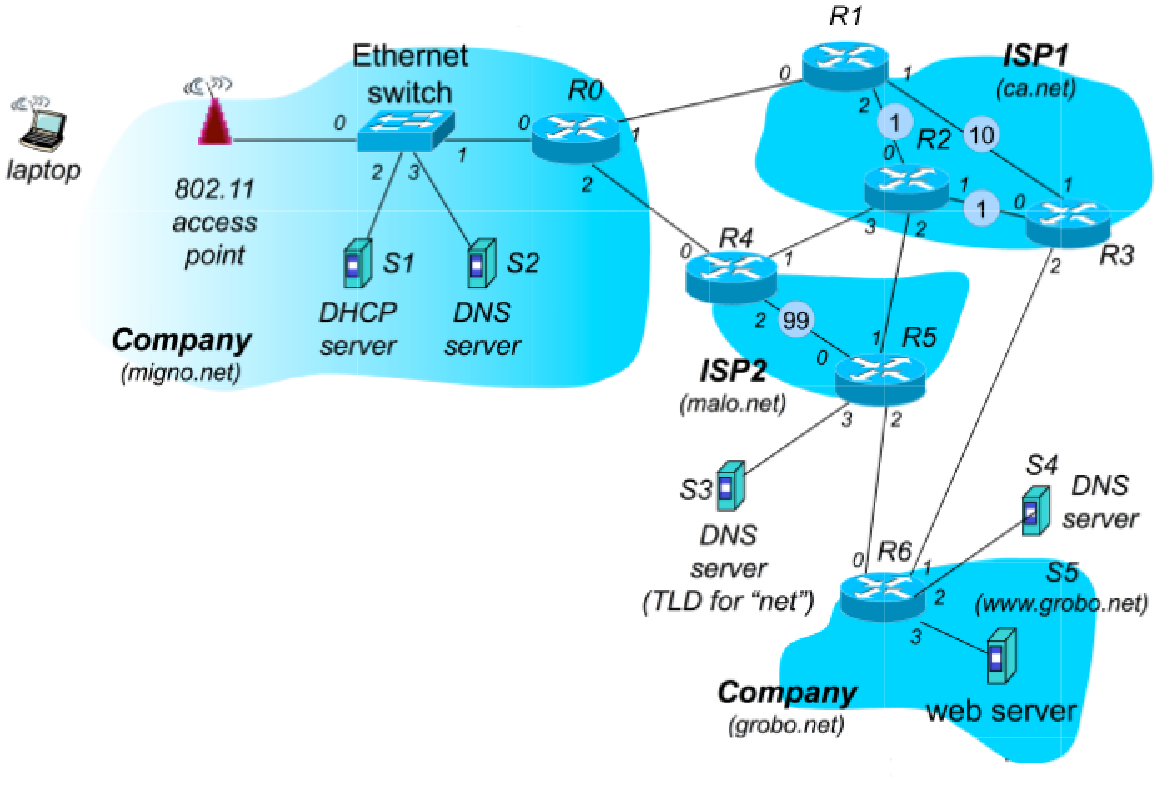
\includegraphics[width=300px]{img_001.pdf}
    \caption{Exemple}
    \end{center}	
\end{figure}

Imaginons que \textit{laptop} cherche à joindre $S_5$ \textit{(\url{www.grobo.net})}, voici les étapes successives se déroulant 
avant et pendant cet échange :
\begin{enumerate}
\item \titre{Lien avec une borne sans-fil}
\begin{itemize}
\item La \term{borne sans-fil} envoie à intervals réguliers des \term{flags} qui sont interceptés par le \textit{laptop}. Un 
\term{flag} contient le \term{SSID}\textit{(Service Set Identifier)} de la borne l'ayant émis.
\item le \textit{laptop} envoie une \term{pro-request} à l'un des \term{SSID} qui lui sont disponibles. \textbf{Il se peut qu'il 
envoie directement une \term{pro-request} s'il connait déjà le \term{SSID}.}
\item La \term{borne sans-fil} répond via une \term{pro-réponse} (avec une phase d'authentification si le réseau est sécurisé) 
contenant, entre autre, le \term{BSSID} \textit{(Basic Service Set Identifier)}. \textbf{Dans le cas d'une \term{pro-request} 
directe, le \term{BSSID} est \textit{"broadcast"} même si l'on connaît le \term{SSID}.}
\end{itemize}
\item \titre{Obtention d'une adresse IP}
\begin{itemize}
\item Le \textit{laptop} \textbf{broadcast} une demande d'adresse \textbf{IP} qui est acheminée au \term{serveur DHCP} 
\textit{(Dynamic Host Configuration Protocol)} \textbf{("DHCP Discover")}. Lorsque la trame arrive à la \term{borne sans-fil} 
elle est transformée d'une trame 802.11 WiFi à une trame 802.3 Ethernet.
\begin{table}[htpd]
\begin{center}
	\begin{tabular}{|c|c|c|c}
	\hline
	MAC SRC & BSSID & MAC DST & ...\\
	\hline
	\end{tabular}
	$\qquad\Rightarrow\qquad$
	\begin{tabular}{|c|c|c}
	\hline
	MAC SRC & MAC DST & ... \\
	\hline
	\end{tabular}
	\caption{802.11 Vs 802.3}
\end{center}
\end{table}
$ $\\Via ce message \textit{DHCP Discover}, le \term{switch Ethernet} apprend l'adresse MAC du \textit{laptop}. Il apprendra 
celle du \term{serveur DHCP} lorsque celui-ci répondra.
\item Le \term{serveur DHCP} répond en broadcastant une proposition d'adresse (broadcast nécessaire, pour que l'adresse ne soit 
pas donnée à 2 équipements différents). La table de switching du \term{switch Ethernet} est désormais :
\begin{table}[h!]
	\begin{center}
	\begin{tabular}{|rc|}
	ADDR MAC & INTERFACE OUT\\
	\hline
	MAC LAPTOP & 0 \\
	MAC DHCP & 2
	\end{tabular}
	\caption{Table de switching du \term{switch Ethernet}}
	\end{center}
\end{table}
\item Le \textit{laptop} répond au \term{serveur DHCP} pour lui signifier qu'il accepte l'adresse.
\item Le \term{serveur DHCP} répond par une confirmation à \textit{laptop}.
\end{itemize}
\item \titre{Accès au serveur DNS pour résoudre \url{www.grobo.net}} \textit{(Domain Name System)} \\
On doit connaître l'adresse MAC du \term{serveur DNS} mais on ne connait que son adresse IP. On utilise alors le protocole 
\textbf{ARP} \textit{(Address Resolution Protocol)} afin d'obtenir cette adresse et on ajoute la réponse reçue (donc l'adresse 
MAC du \term{serveur DNS}) dans la table de switching.
\item \titre{Résolution de \url{www.grobo.net}}\\
Dans notre cas, on va déléguer la tâche au \term{serveur DNS} (qui sert de cache en général) de manière itérative (comme en 
pratique) en lui demandant l'adresse IP correspondant à \url{www.grobo.net}. \textit{(On suppose que $S_2$ connait $S_3$)}
\begin{itemize}
\item le \term{serveur DNS} ($S_2$) demande au \term{TLD}\textit{(Top Level Domain)} pour ".net" ($S_3$) s'il connaît 
\url{www.grobo.net}.
\item Celui lui répond qu'il devrait demander à $S_4$ qui lui répond qu'il connaît et qu'il est joignable à $S_5$.
\end{itemize}
\item \titre{Calcul du chemin jusque $S_3$}
$S_2$ connaît de manière statique le lien vers $R_0$ pour joindre internet ($0.0.0.0/0$, préfixe par défaut).
\begin{itemize}
\item \titre{inter-AS} \\
Via \term{BGP} \textit{(Border Gateway Protocol)}, chaque routeur en bordure d'un réseau proprage la liste des préfixes qu'il 
peut atteindre ainsi que la liste des \term{AS} \textit{(Autonomous System)} par lequel il faut passer pour atteindre une 
adresse dans chacun de ces préfixes \textit{(AS-PATH)}. \\
De cette manière, $R_0$ sait quel chemin est le plus court pour joindre $S_3$ (s'il y en a plusieures, il effectue un processus 
de décision pour en choisir un).
\begin{figure}[h!]
    \begin{center}
    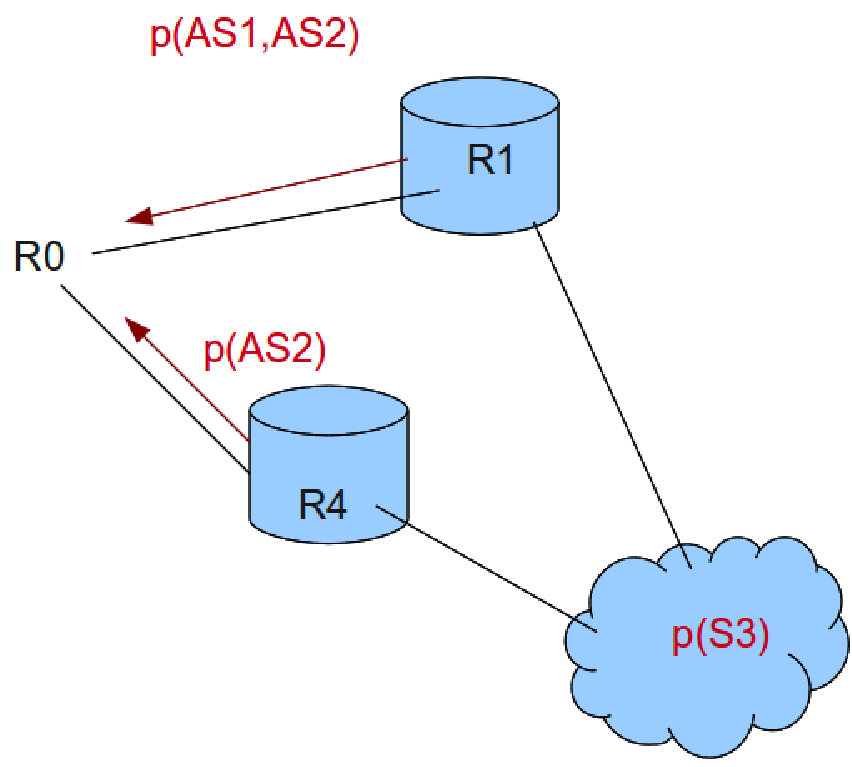
\includegraphics[width=150px]{img_BGP.pdf}
    \caption{Topologie et Messages BGP $R_0$, $R_1$ et $R_4$}
    \end{center}	
\end{figure}
$R_0$ passera donc par $R_4$.
\item \titre{intra-AS} \\
Il convient ici de considérer les poids des liens (via \term{OSPF} \textit{(Open Shortest Path First)}
\end{itemize}
Pour rappel, un routeur a 4 moyens d'apprendre une route (par ordre de priorité) :
\begin{enumerate}
\item de manière \textbf{statique} : rentrée par l'opérateur manuellement,
\item de manière \textbf{directe} : par la topologie du réseau (les cables connectés),
\item de manière \textbf{intra-domaine} via \term{OSPF},
\item de manière \textbf{extra-domaine} via \term{BGP}.
\end{enumerate}
\begin{itemize}
\item $S_2$ contacte $S_3$ comme dit précédemment puis effectue le même raisonnement pour $S_4$.
\item $S_2$ contacte donc $S_4$. Via le routage, $R_0$ reçoit 2 routes d'$AS-PATH$ de même longueur ($AS3,AS1$ et $AS3,AS2$). Il 
effectue un "tie-break" c'est-à-dire qu'il fait un choix parce qu'il faut bien en faire un (en général il prend l'adresse 
\textbf{IP} la plus petite.
\end{itemize}
\item $S_2$ connaît à présent l'adresse \textbf{IP} de $S_5$ (qui correspond à \url{www.grobo.net}) et la donne au 
\textit{laptop}. 
Celui-ci sait qu'elle n'est pas sur le réseau local, il effectue donc une requête \textbf{ARP} pour obtenir la \textit{gateway}. 
En effet il connaît l'adresse \textbf{IP} de celle-ci grâce au \term{serveur DHCP} qui lui a communiqué les adresses \textbf{IP} 
des routeurs passerelles du réseau. La table de routage de \textit{laptop} est donc comme suit :
\begin{table}[h!]
\begin{center}
\begin{tabular}{l|r|r}
Préfixe & Interface Out & Passerelle \\
\hline
$10.0.0/24$ & $wlan0$ & \\
$0.0.0.0/0$ & $wlan0$ & $p(R_0)$\\
\end{tabular}
\end{center}
\caption{Table de routage de \textit{laptop}}
\end{table}
\item $S_2$ envoie sa requête à $S_5$.
\end{enumerate}

\subsection{Traffic Engineering}

Les chemins les plus courts sont calculés via \textbf{Dijkstra} ce qui assure que chaque paquet utilisera le plus court chemin 
pour être transmis. Le problème à ça c'est que le chemin le plus court sera le seul et unique utilisé. On peut avoir envie de 
répartir équitablement le trafic sur les 2 liens de sorties.

\begin{figure}[h!]
    \begin{center}
    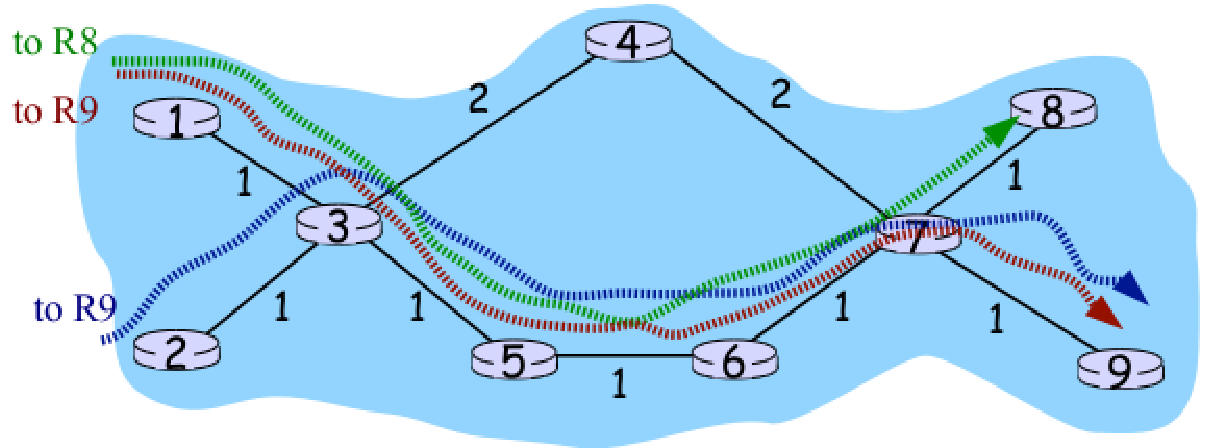
\includegraphics[width=200px]{img_002.pdf}
    \caption{Exemple d'emploi du plus court chemin à mauvais escient}
    \end{center}	
\end{figure}

On peut, pour résoudre à cela, par exemple, modifier les coûts du second chemin afin que les coûts des 2 chemins soient 
identiques. Il faut alors également modifier \textbf{Dijkstra} pour qu'il garde tous les chemins de coût minimum (et pas un 
seul). C'est l'idée du protocole \term{ECMP} \textit{(Equal Cost Multiple Path)}. On choisit entre ces chemins de manière 
aléatoire ou avec le \term{round-robin}. La manière aléatoire n'est pas adaptée car elle n'est pas \textbf{TCP-friendly}, en 
effet, on ne peut assurer qu'un flux \textbf{TCP} restera sur le même chemin. Le \term{round-robin} consiste lui à assigner un 
des chemins à chaque flux \textbf{TCP} différent rencontré. Pour rappel, un flux \textbf{TCP} est identifié par le quadruplet 
$(ADD\ SRC,\ PORT\ SRC,\ ADD\ DST,\ PORT\ DST)$. En parallèle avec chaque lookup \textbf{IP} il faudra donc calculer une valeur 
de hashage pour le quadruplet afin de déterminer le chemin à utiliser.\\

Cette méthode fonctionnera bien s'il y a plusieurs petits flots (ne marche pas avec peu de gros flots) et si il y a beaucoup de 
chemins de même coût (totalement dépendant de l'assignation des coûts). La fonction de hashage doit être bien déterminée pour 
être assez discriminante pour ne pas assigner la route à flots très proches (mêmes couples d'adresses par exemple). De plus, si 
tous les routeurs utilisent la même fonction de hashage, cela crée une \textbf{polarisation} du réseau ; en effet, pour chaque 
routeur, on va choisir la même interface de sortie. \textit{(On peut remédier à cette polarisation en ajouter le routeur ID dans 
la fonction de hashage)} \\

D'autres mécanismes, différents du \term{ECMP} existent. On peut modifier les poids des noeuds afin de minimiser le ratio 
charge/capacité pour chaque noeud en favorisant les chemins de même coût. Cette méthode requiert de connaître la matrice de 
trafic ce qui n'est pas toujours le cas. On peut aussi utiliser le routage explicite : "Tel flux prend tel chemin" ou encore 
un autre schéma de forwarding (comme \textbf{MPLS} \textit{(Multiprotocol Label Switching)}) ou un protocole de signalisation 
pour installer un état (comme \textbf{RSVP-TE} \textit{(Resource reSerVation Protocol -Traffic Engineering))}.

\section{Introduction au routage inter-domaine}

\subsection{Objectifs fondamentaux}

\begin{itemize}
\item Permettre de transmettre des paquets IP par le meilleur chemin
  lorsqu'il est nécessaire de passer par plusieurs domaines de transit
  (souvent, ``meilleur chemin'' revient à ``chemin le moins cher'')
\item Prendre en compte les politiques de routage de chaque domaine
\item Autonomie (à l'intérieur d'un domaine, les opérations sont
  effectuées indépendamment des autres, chaque domaine peut faire
  tourner son propre IGP)
\item Cacher la topologie détaillée des domaines de transit (routage
  hiérarchique, nécessaire car le graphe inter-domaines possède des
  millions de noeuds)
\end{itemize}

\subsection{Définitions}

\begin{itemize}
\item Un système autonome (AS) est un réseau sous l'administration
  d'une entité unique (BELNET, Abilène, ...)
\item Un préfixe est un ensemble d'adresses IP spécifié dans la
  notation CIDR (193.190.192/22 (UMons), ...)
\item Lien privé: câble reliant deux routeurs appartenant à deux AS
  différents
\item Connection via un point d'interconnexion: En général via un
  switch Gigabit (ou plus)
\end{itemize}

\subsection{Politiques de routage}

Il y a deux politiques principales:

Un lien client-vendeur (un client C achète de la connectivité internet
à un provider P)

Un lien à coût partagé (les domaines X et Y se mettent d'accord pour
échanger des paquets en utilisant un lien direct ou un point
d'interconnexion)

Bien sûr, des politiques plus complexes sont possibles (et existent)

\paragraph{Matrice de politique de transit}

\begin{tabular}{c|c|c|c|c|}
  \multicolumn{2}{c|}{} & \multicolumn{3}{c|}{Vers} \\
  \cline{3-5}
  \multicolumn{2}{c|}{} & Provider & Pair & Client \\
  \hline
  \multirow{3}{*}{De} & Provider & \color{red}{Non} & \color{red}{Non} &
     \color{green}{Oui} \\
  \cline{2-5}
  & Pair & \color{red}{Non} & \color{red}{Non} & \color{green}{Oui} \\
  \cline{2-5}
  & Client & \color{green}{Oui} & \color{green}{Oui} & \color{green}{Oui} \\
  \hline
\end{tabular}

\paragraph{RPSL}

Pour faire appliquer ces règles (ou d'autres), un mécanisme de filtres
est mis en place. Les administrateurs de réseaux peuvent donc
appliquer un ou plusieurs filtres à chaque ``porte'' de leur réseaux:
des filtres d'imports, qui permettent de limiter le trafic entrant, et
des filtres d'export, qui permettent de limiter le trafic sortant.

Ces filtres sont en général exprimés dans un langage spécifique au
vendeur du routeur, le standard est RPSL (Routing Policy Specification
Language)

Exemples simples de syntaxe RPSL:

\begin{verbatim}
import: from AS# accept list_of_AS

import: from BELNET accept UMONS
import: from LEVEL3 accept ANY

export: to AS# announce list_of_AS

export: to UMONS announce ANY
export: to LEVEL3 announce UMONS UCLOUVAIN ...
\end{verbatim}

\section{BGP}

Il s'agit du standard pour le routage inter-domaines

Permet à chaque AS ...

\begin{itemize}
\item ... de savoir si tel ou tel préfixe peut être atteint depuis les
  AS voisins
\item ... de propager cette information dans chaque routeur interne à
  l'AS
\item ... de déterminer les ``bonnes'' routes vers les sous-réseaux en
  se basant sur l'information d'atteignabilité et la politique de
  l'AS.
\end{itemize}

BGP permet également aux sous-réseaux de signaler leur existence.

Pour remplir ces objectifs, BGP utilise un protocole de vecteurs de
distance et des mises à jour incrémentales. (Avertisement de mise à
jour seulement quand l'information change)

\subsection{Sessions}

\paragraph{Principe}

Les paires de routeurs BGP s'échangent des routes sur leur connexion
TCP semi-permanente: la session BGP

Les routeurs disposant d'une session BGP sont appelés pairs BGP ou
voisins BGP.

Le port par défaut pour les sessions BGP est 179.

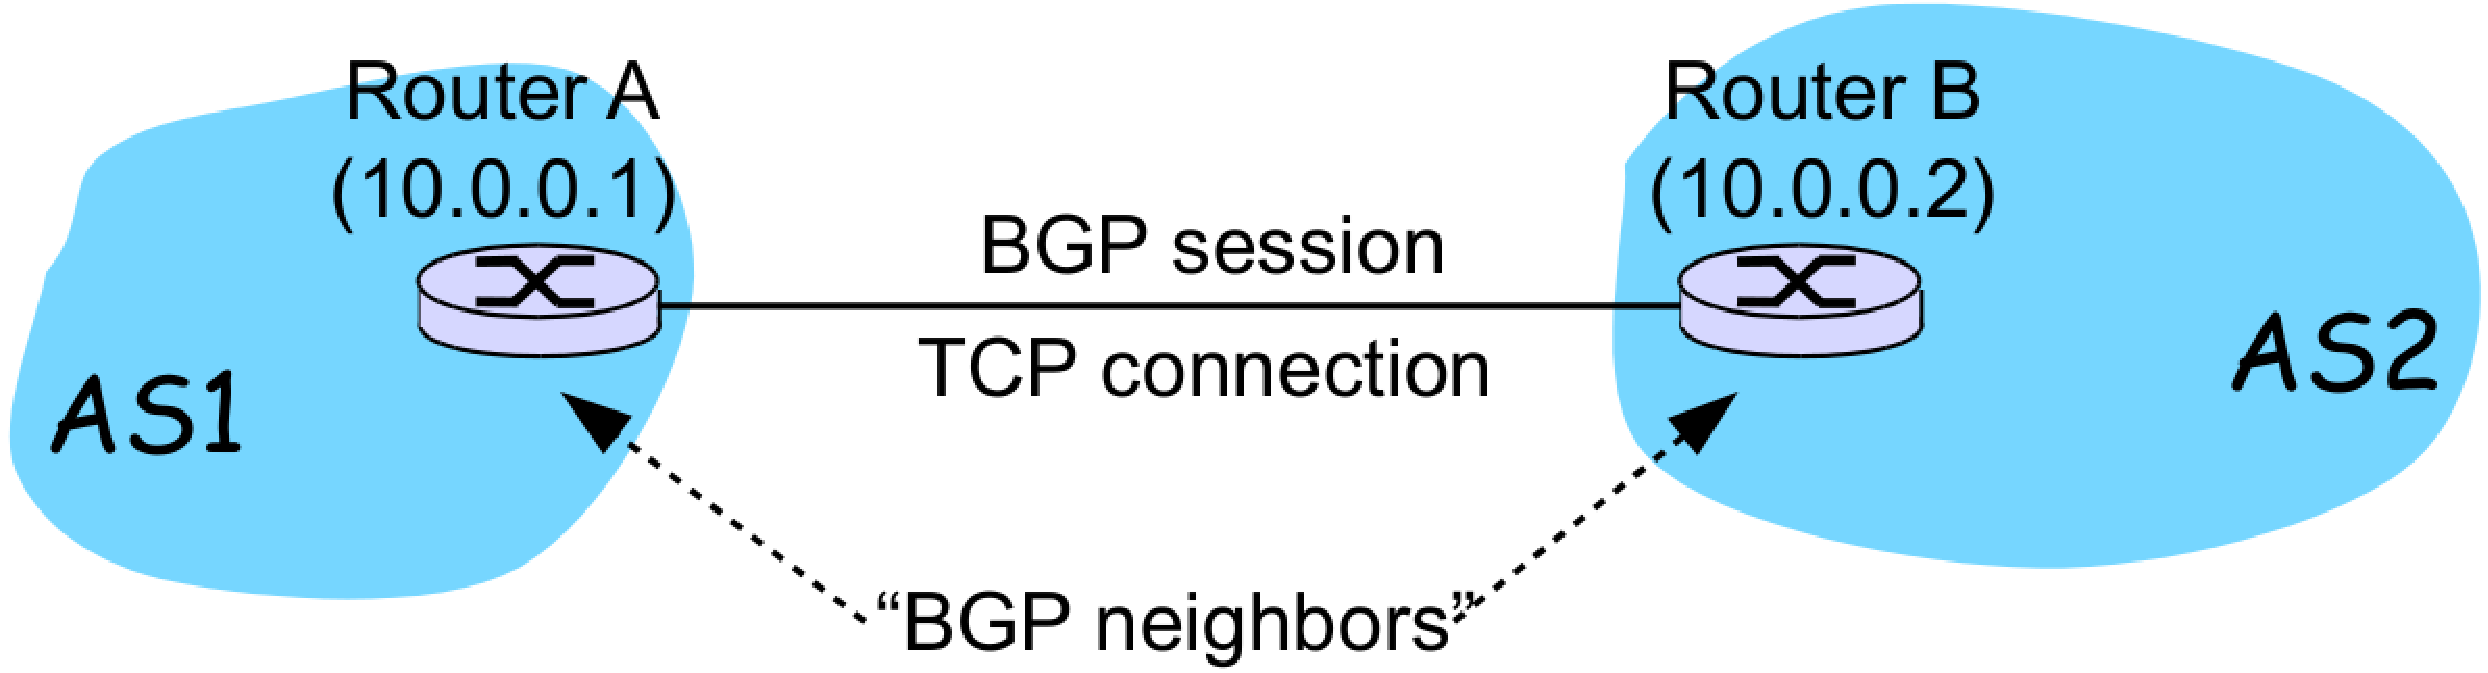
\includegraphics[width=\textwidth]{fab_001.pdf}

\paragraph{Configuration d'une session BGP}

Préliminaire: les deux routeurs doivent être capables de s'atteindre

CISCO:

\begin{verbatim}
# router bgp [ASN]
# neighbor [IP_VOISIN] remote-as [ASN_VOISIN]
\end{verbatim}

Juniper:

\begin{verbatim}
routing-options {
  autonomous-system [ASN];
}

protocols {
  bgp {
    group [NOM_GROUPE_VOISINS] {
      peer-as [ASN_VOISIN];
      type external;
      neighbor [IP_VOISIN];
    }
  }
}
\end{verbatim}

\subsection{Messages}

4 grands types de messages dans le protocole BGP:

\begin{itemize}
\item OPEN (ouverture de session, éventuellement authentification)
\item UPDATE (avertissement des chemins neufs / obsolètes)
\item KEEPALIVE (maintient une connexion, ack du OPEN)
\item NOTIFICATION (erreurs, fermeture de connexion)
\end{itemize}

Le header d'un message BGP est composé des champs suivants:

\begin{itemize}
\item Marker (16 bytes) inutilisé, ne doit contenir que des 1
\item Longueur (2 bytes) longueur du paquet, header compris
\item Type (1 byte) 1=OPEN, 2=UPDATE, 3=NOTIFICATION, 4=KEEPALIVE,
  5=ROUTE REFRESH
\item Corps du message
\end{itemize}

\paragraph{Message OPEN}

Le corps est composé des champs suivants:

\begin{itemize}
\item Version (1 byte) vaut 4 (00000100)
\item ASN de l'émetteur (2 bytes)
\item Temps d'attente (2 bytes)
\item Identifiant BGP (4 bytes) Adresse IP d'une des interfaces du
  routeur émetteur
\item Longueur des paramètres optionnels (1 byte)
\item Paramètres optionnels (triplets [type, longueur, valeur])
\end{itemize}

\paragraph{Message UPDATE}

Le corps est composé des champs suivants:

\begin{itemize}
\item Nombre de routes obsolètes (2 bytes)
\item Routes obsolète (variable)
\item Longueur des attributs de chemins (2 bytes)
\item Attributs de chemins (variable)
\item Network Layer Reachability Information [NLRI] (variable)
\end{itemize}

\subsection{Routes}

\paragraph{Définition}

Une route est la combinaison d'un préfixe de destination et
d'attributs de chemin, elle est transportée par un message UPDATE, le
préfixe de destination est spécifié dans la partie NLRI du message et
un routeur BGP annonce une seule route par préfixe de destination.

\paragraph{Avertissements de routes}

Ils proviennent de diverses sources:

\begin{itemize}
\item Routes statiques, configurées manuellement dans le routeur
\item Redistribution de route (apprises par un protocole de routage
  intra-domaine, iBGP par exemple), mais c'est une mauvaise habitude
  vu que les instabilités intra-domaine seraient répercutées à
  l'extérieur et risqueraient de rendre le BGP global instable
\item Apprentissage de routes depuis un autre routeur BGP (chaque
  noeud BGP avertit ses voisins de ses meilleures routes)
\end{itemize}

\paragraph{Abandon de routes}

Principe: quand une destination n'est plus atteignable, un routeur BGP
doit en avertir ses voisins.

Les messages UPDATE sont utilisés pour informer qu'une route n'est
plus disponible, on appelle ces messages WITHDRAW alors que,
strictement, aucun message WITHDRAW n'existe dans la spécification
BGP. Un WITHDRAW ne doit être envoyé que pour des routes précédemment
annoncées.

Un WITHDRAW implicite est un message UPDATE modifiant juste un
attribut de la route (c'est-à-dire que la destination peut toujour
être atteinte, mais avec d'autres paramètres car il faut passer par
d'autres routeurs BGP par exemple).

\subsection{Attributs des chemins}

Une route peut contenir plusieurs attributs; les deux les plus
importants sont NEXT-HOP (IP du prochain routeur BGP sur la route) et
AS-PATH (liste des ASN des routeurs suivants sur la route)

L'AS-PATH, en plus de servir de métrique, permet d'éviter les boucles
de routage: un routeur BGP voyant son propre ASN dans l'AS-PATH ne
considérera pas cette route.

Attributs de chemins standardisés

\begin{tabular}{l|c|c|c|c|c|}
  Nom & Code & Implémentation & attribut & Transitif \\
  & & obligatoire & obligatoire & \\
  \hline
  ORIGIN & 1 & Y & Y &  \\
  \hline
  AS-PATH & 2 & Y & Y & \\
  \hline
  NEXT-HOP & 3 & Y & Y & \\
  \hline
  MED (Multi Exit Discriminator) & 4 & & & \\
  \hline
  LOCAL\_PREF & 5 & Y & & \\
  \hline
  ATOMIC\_AGGREGATE & 6 & Y & & \\
  \hline
  AGGREGATOR & 7 & & & Y \\
  \hline
  COMMUNITIES & 8 & & & Y \\
  \hline
  ORIGINATOR\_ID & 9 & & & \\
  \hline
  CLUSTER\_LIST & 10 & & & \\
  \hline
  EXTENDED\_COMMUNITIES & 16 & & & \\
  \hline
\end{tabular}

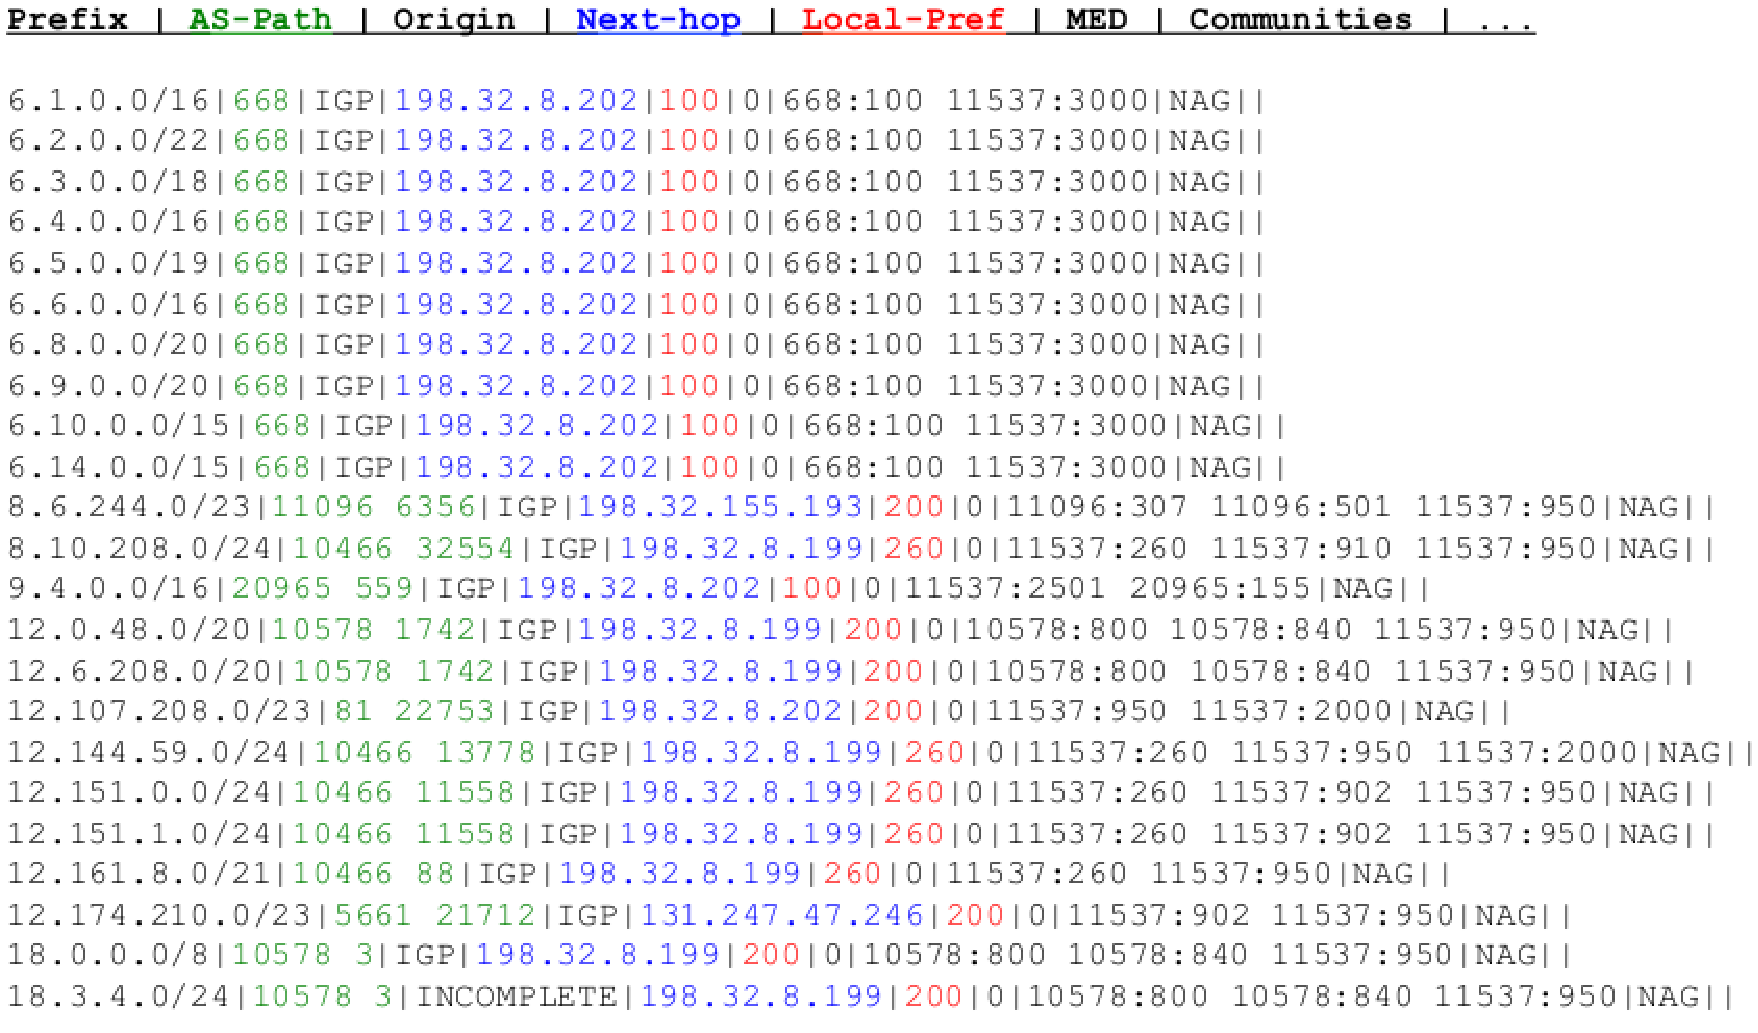
\includegraphics[width=\textwidth]{fab_002.pdf}

\subsection{Machine à états finie}

Le but de la machine à étatss BGP est de s'assurer de la gestion
correcte des messages BGP comme de la robustesse des sessions
BGP. Toute implémentation pour un routeur BGP doit suivre le même
comportement que la machine à états.

La machine est composée de 6 états:

\begin{itemize}
\item Idle (état initial)
\item Connect (tentative d'initiation de connexion TCP)
\item Active (écoute de connexions TCP entrantes)
\item OpenSent (OPEN envoyé, attente d'un OPEN entrant)
\item OpenConfirm (OPEN reçu, KEEPALIVE envoyé, attente d'un KEEPALIVE
  entrant)
\item Established (En marche, échange de KEEPALIVE et de UPDATE)
\end{itemize}

Et de 3 timers:

\begin{itemize}
\item ConnRetry (Espace les tentatives de connexion TCP)
\item HoldTimer (Assure l'activité de la session BGP)
\item KeepAlive (Envoie des KEEPALIVE régulièrement)
\end{itemize}

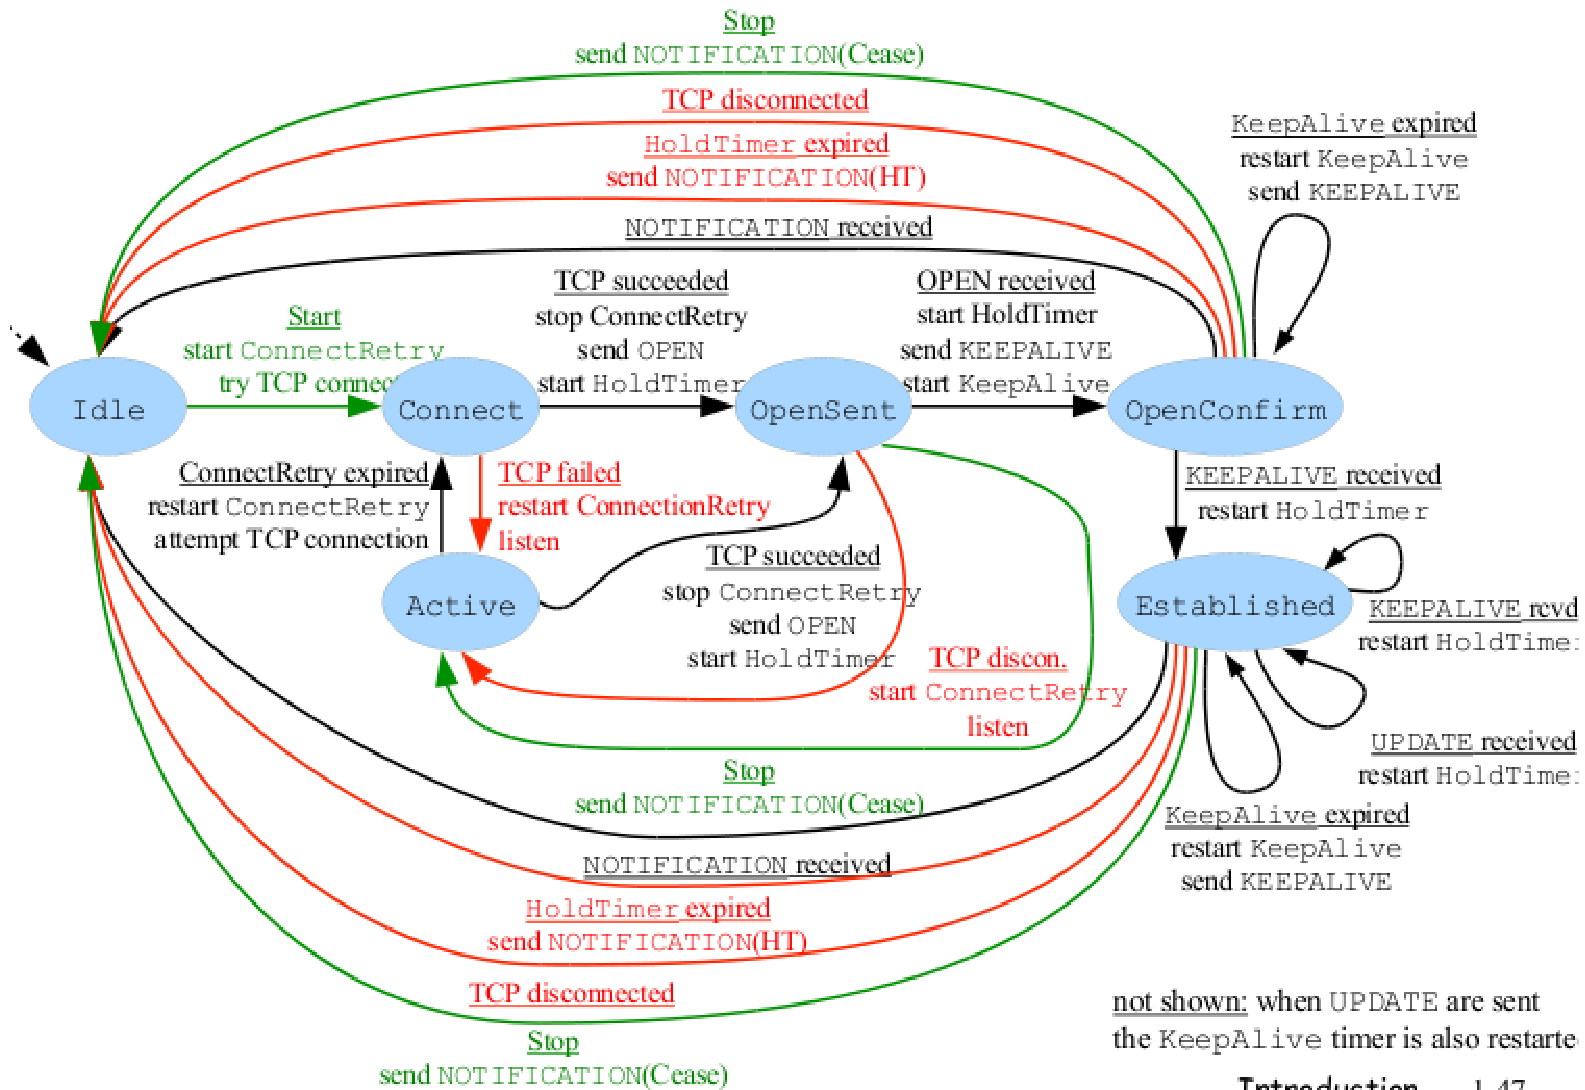
\includegraphics[width=\textwidth]{fab_003.pdf}

\subsection{Processus de décision}

Un routeur recevra souvent plusieurs routes pour joindre un même
préfixe. Il doit alors choisir une unique meilleure route à
communiquer à ses voisins.

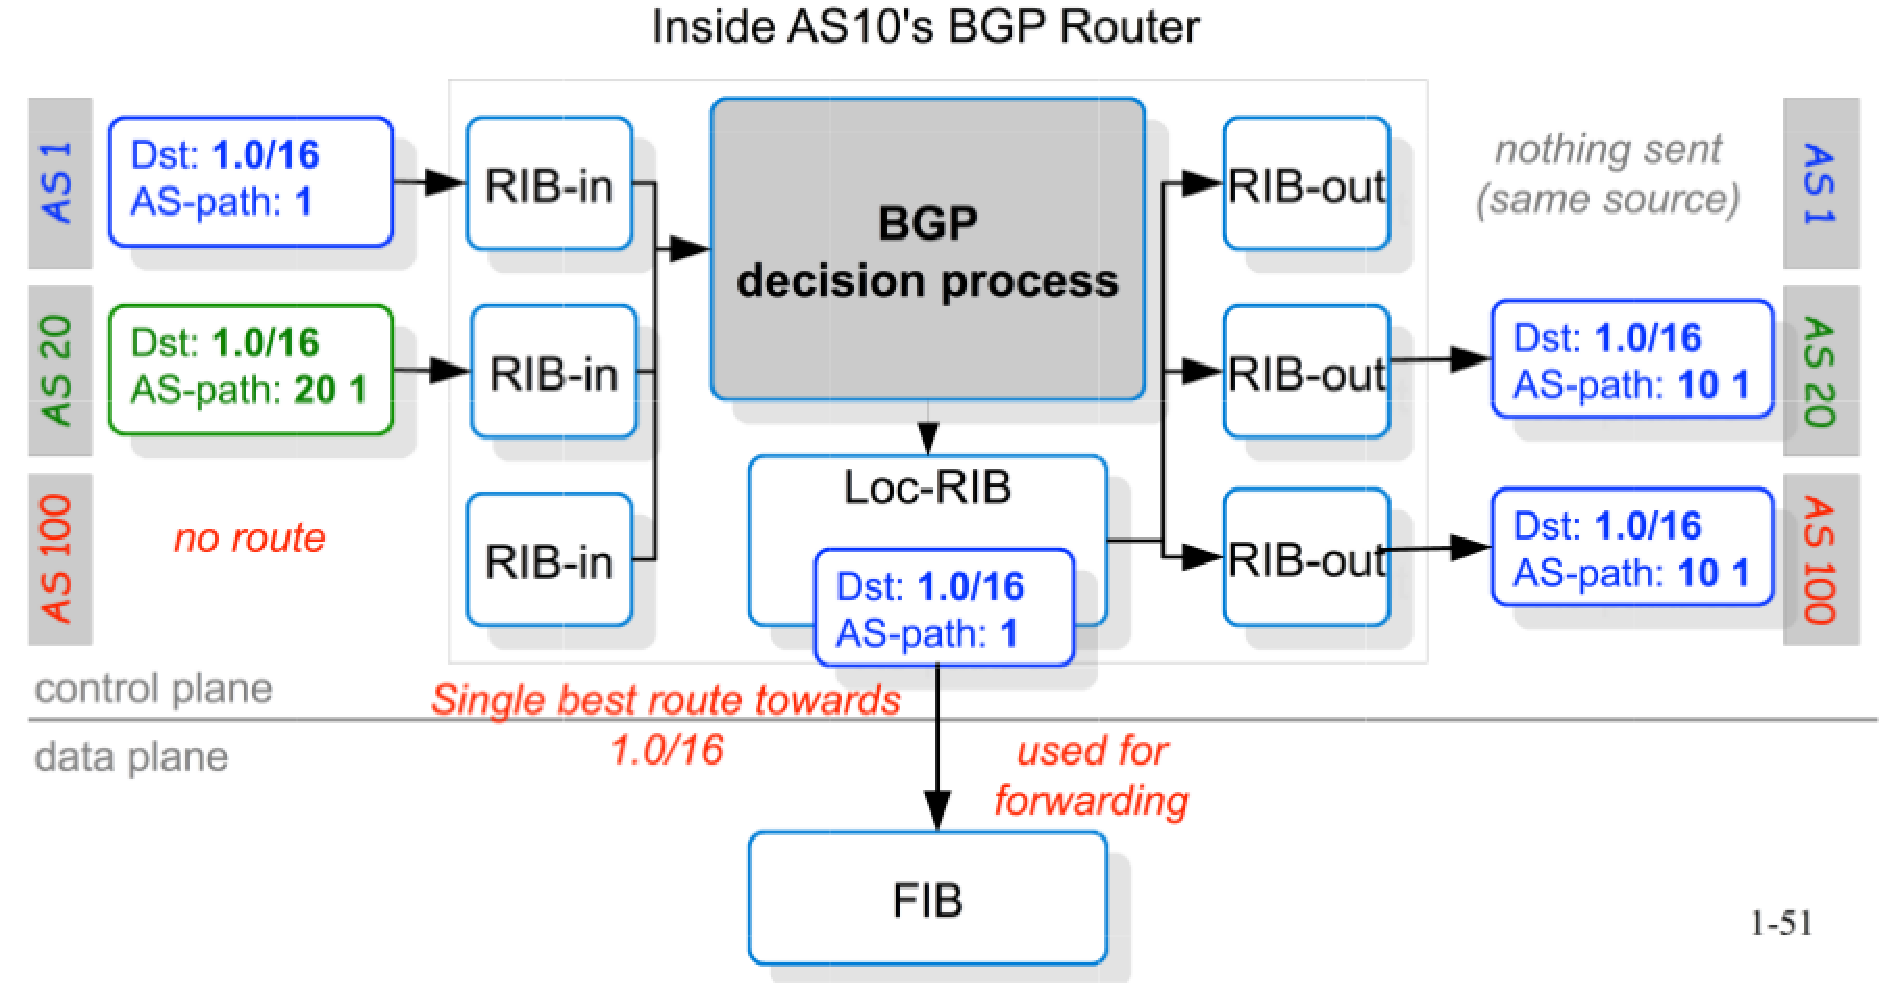
\includegraphics[width=\textwidth]{fab_004.pdf}

Le processus de décision est composé d'une série de règles qui va
réduire l'ensemble des routes admissibles pour un préfixe donné
jusqu'à ce qu'il n'en reste qu'une, ce sera la meilleure route, qui
sera ensuite communiquée aux voisins du routeur (en accord avec la
politique de l'AS bien entendu).

Le processus simplifié ressemble à ceci:

\begin{itemize}
\item Ignorer si le NEXT-HOP n'est pas joignable
\item Préférer les routes ayant un LOCAL-PREF supérieur
\item Préférer les routes ayant un AS-PATH plus court
\item Tie-break
\end{itemize}

Voici le processus de décision complet:

\begin{enumerate}
\item Ignorer si le NEXT-HOP n'est pas joignable
\item Préférer les réseaux originaires du réseau local
\item Préférer les routes ayant un LOCAL-PREF supérieur
\item Préférer les routes ayant un AS-PATH plus court
\item Préferer les ORIGIN les plus bas
\item Préférer les MED les plus bas
\item Préférer eBGP par rapport à iBGP
\item Préférer le NEXT-HOP le plus proche
\item Préférer le ROUTER-ID / ORIGINATOR-ID le plus bas
\item Préférer le CLUSTER-LIST le plus court
\item Préférer l'adresse du voisin la plus petite
\end{enumerate}

On s'en doute, les trois derniers points sont des tie-breaks.

\subsection{Filtres de routage}

\paragraph{Objectifs}

\begin{itemize}
\item Influencer le classement des routes
\item Empêcher certaines routes d'être redistribuées à certains voisins
\item Rejeter une route d'un voisin spécifique
\end{itemize}

\paragraph{Principes}

\begin{itemize}
\item Ajouter des filtres d'import/export au modèle de routage BGP
  pour chaque voisin
\item Filtres d'import (in-filters): sélectionner les routes
  acceptables et changer leurs attributs
\item Filtres d'export (out-filters): sélectionner les routes
  redistribuables et changer leurs attributs
\item Les filtres sont spécifiés dans un langage spécifique au vendeur
  du matériel
\end{itemize}

Un filtre est un ensemble de prédicats qui mènent à un ensemble
d'actions.

\paragraph{Exemples de prédicats}

\begin{itemize}
\item match destination prefix against IP prefix
\item match next-hop against IP address / prefix
\item test existence of an ASN in AS-PATH
\item match AS-PATH against regular expression
\item ...
\end{itemize}

\paragraph{Exemples d'actions}

\begin{itemize}
\item Accept / reject the route
\item Set / Increase / Decrease LOCAL-PREF
\item Prepend AS-PATH
\item Set MED
\item Add / Remove community
\item Remove private ASN from AS-PATH
\item ...
\end{itemize}

\paragraph{Exemple d'application}

Un AS possède souvent plusieurs liens vers son provider. Un lien
principal qui doit être utilisé autant que possible et un lien
secondaire qui doit être utilisé lorsque le lien secondaire ne
fonctionne pas.

On peut donc configurer un filtre donnant une priorité plus grande aux
routes fournies par le routeur de la route principale

\begin{verbatim}
import: from AS2 RB at RA set localpref=200;
import: from AS2 RC at RA set localpref=100;
\end{verbatim}

Cela aura pour effet de donner une priorité plus grandes aux routes
fournies par le routeur RB, alors qu'elles sont en fait équivalentes à
celles fournies par le routeur RC en termes d'étendue (pas forcément
en termes de rapidité / bande passante)

\paragraph{Autre exemple d'application}

L'attribut LOCAL-PREF est souvent utilisé pour représenter les
relations économiques entre les AS, elles sont définies de telle sorte
qu'on ait:

\[rank(customer routes) > rank(peer routes) > rank(provider routes)\]

Remarquons que cela permet l'utilisation de routes asymétriques pour
l'aller et le retour, comme l'illustre le schéma suivant:

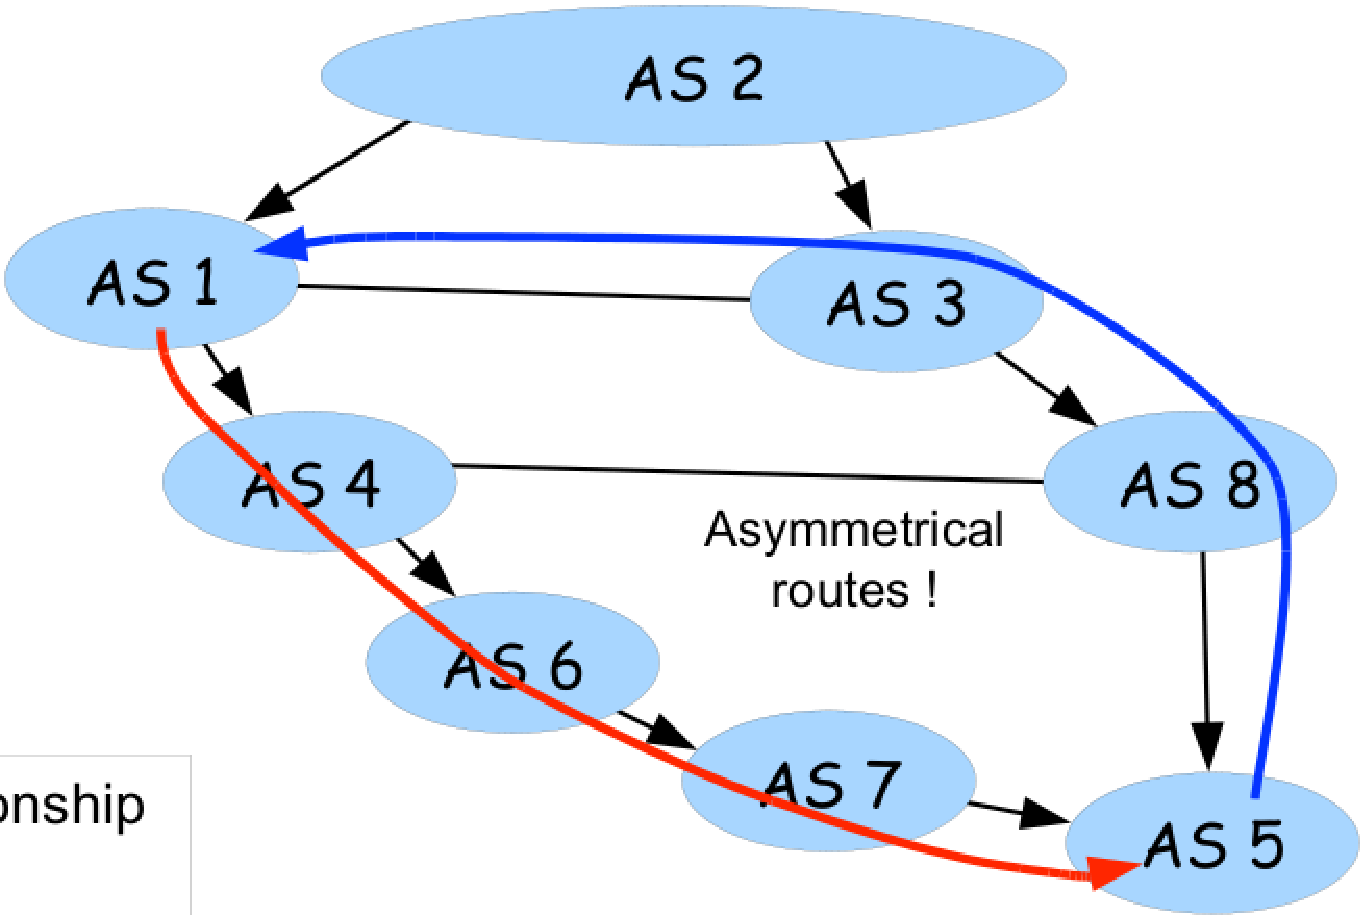
\includegraphics[width=\textwidth]{fab_005.pdf}

Dans cet exemple, les paquets devant aller de AS8 à AS1 ne passent pas
par AS4 (c'est pourtant plus avantageux pour AS8 !) car AS4 n'a pas
annoncé qu'il avait une route vers AS1 à AS8.

\paragraph{Filtres automatiques du protocole}

En plus des filtres définis par la configuration, les routeurs BGP
appliquent les filtres suivans automatiquement:

\begin{itemize}
\item LOCAL-PREF est enlevé des routes avant qu'elles soient transmises
\item L'ASN du routeur est ajoutée au début de l'AS-PATH des routes
  avant qu'elles soient transmises
\item Une route contenant l'ASN d'un voisin ne sera pas transmise à ce
  voisin (sender-side loop detection)
\item l'attribut NEXT-HOP est mis à jour avant que la route ne soit
  transmise
\end{itemize}

\subsection{BGP interne (iBGP)}

iBGP permet aux routeurs d'un AS de s'échanger des routes, il s'agit
en fait d'une version modifiée de BGP dont les principales différences
sont:

\begin{itemize}
\item LOCAL-PREF n'est transporté que sur les sessions iBGP (pas eBGP)
\item les filtres d'import/export ne sont définis que pour les
  sessions eBGP
\item les routes apprises dans les sessions iBGP ne peuvent pas être
  redistribuées sur d'autres sessions iBGP
\item les attributs NEXT-HOP et AS-PATH ne sont mis à jour que lorsqu
  la route est envoyée à travers une session eBGP
\end{itemize}

Afin que tout se passe bien dans l'AS, il est préférable que tous les
routeurs internes fassent tourner BGP (on appelle cela un full mesh).

Sinon, on peut:

\begin{itemize}
\item utilier des tunnels (MTU réduit, routeurs ``chargés'' par
  l'encapsulation/décapsulation des paquets aux extrémités du tunnel,
  configuration statique nécessaire (manuelle))
\item redistribuer les routes BGP dans l'IGP (très mauvais pour la
  montée en charge, danger de réinjecter les routes dans BGP avec un
  AS-PATH de longueur unitaire (AS7007)
\end{itemize}

\paragraph{En résumé}

Le rôle d'IGP est de distribuer la topologie interne et les adresses
internes à l'intérieur de l'AS, tandis que le rôle d'iBGP est de
distribuer les routes vers les destinations extérieures apprises par
eBGP aux autres routeurs de l'AS.

Les sessions iBGP peuvent être établies grâce aux route IGP.

\paragraph{Préférer eBGP à iBGP dans le processus de décision}

Aussi appelé ``routage de la patate chaude'', un routeur devrait
tenter de se débarasser des paquets à destination d'autres domaines
(AS) aussi rapidement que possible.

\paragraph{Choisir le next-hop le plus proche}

Toujours dans l'optique du ``routage de la patate chaude'', lorsque
les règles précédentes du processus de décision amènent à des
égalités, on utilise le next-hop (IGP, s'entend) le plus proche.

\paragraph{Choisir le MED le plus faible}

Alors que les deux règles qu'on vient de voir favorisent l'émetteur
des paquets, le MED permet au futur récepteur d'influencer l'émetteur
sur la route à choisir. Cependant l'émetteur peut choisir de
simplement ignorer le MED. Celui qui annonce une route vers un certain
préfixe peut ainsi joindre à la route un MED indiquant quelle route il
préfère à une autre (plus le MED est faible, plus la route est
favorable pour l'annonceur de la route)

Le MED impose toutefois un problème supplémentaire: deux MED ne
peuvent être comparés que si les routes auxquelles ils appartiennent
proviennent du même AS.

La règle ``Choisir le MED la plus faible'' dans le processus de
décision va donc consister à garder, pour chaque AS ayant encore des
routes ``en lice'', celle ayant le MED le plus faible.

\subsection{Ingénierie de trafic basée sur BGP}

\subsection{Multi-homing}

Au début de sa vie, un AS, connecté à un seul provider, utilise un ASN
privé (de 64512 à 65535) et est complètement caché derrière son ISP.

Ensuite, l'AS veut devenir multi-homed et obtient un ASN public. l'ISP
doit alors prévenir ses autres clients qu'un nouvel AS existe et faire
ainsi grossir la taille des tables de routage globales.

\paragraph{Aggrégation}

BGP peut agréger les routes reçues, l'attribut AS-PATH est une
AS-séquence formée d'AS-ensembles, la plupart des AS-ensembles sont
constitués d'un seul élément, Un AS-ensemble n'est pas ordonné et
compte pour une longueur de 1.

L'information sur le chemin réel est perdue lorsque les AS-ensembles
sont utilisés; mais l'aggrégation permet le diminution de la taille
des tables de routage. Une liste des ``mauvais élèves'' n'utilisant
pas l'aggrégation est maintenue. On estime que, si l'aggrégation était
parfaitement utilisée, on pourrait réduire de 50\% la taille des
tables de routage.

\paragraph{Revenons à notre AS, il devient multi-homed}

Comme son ISP initial utilisait l'aggrégation, et que le nouvel ISP ne
l'utilise pas (il ne peut pas, le préfixe du client n'entrant pas dans
son propre préfixe), l'AS-PATH proposé par le nouvel ISP sera toujours
utilisé (le préfixe est plus précis).

De son côté, l'ISP initial devrait arrêter d'agréger le préfixe du
client, sinon le client ne recevra pas les paquets des autres clients
agrégés (Le provider va annoncer une route contenant l'AS du client,
le client va donc la rejeter, et n'aura pas connaissance des routes
vers les autres clients du provider. Idem si les routes passent par
d'autres routeurs: l'AS du client restera dans l'AS-PATH et la route
sera donc systématiquement jetée (ou même pas reçue par le client avec
le sender-side loop detection)

\paragraph{Comment limiter l'expansion des tables de routage ?}

Sur le long terme, IPv6 apportera une solution, en définissant une
meilleure notion de multi-homing.

\subsection{Gestion du trafic via BGP}

On aimerait par exemple que le trafic vers un certain préfixe passe
par un fournisseur, tandis que le trafic vers un autre préfixe passe
par un autre fournisseur, ou alors privilégier un lien par rapport à
un autre, mais garder l'autre comme back-up. Plusieurs techniques sont
envisageables:

\begin{itemize}
\item Annonces sélectives: N'annoncer certain préfixes que sur
  certains liens (Expansion des tables de routage, que se passe-t-il
  si un lien lache ?)
\item Préfixes plus spécifiques: Annoncer un préfixe global sur chaque
  lien, et un préfixe plus spécifique sur chaque lien (Expansion des
  tables de routage, mais plus robuste)
\item AS-PATH prepending (rendre l'AS-PATH artificiellement plus long
  en ajoutant plusieurs fois son ASN à l'AS-PATH selon le lien sur
  lequel on se trouve à l'aide d'un filtre)
\end{itemize}

\subsection{Résistance à la montée en charge}

\paragraph{Objectifs}

\begin{itemize}
\item Réduire le nombre de sessions iBGP (full mesh !), deux
  techniques pour cela: les confédérations et la réflection de routes
\item Permettre une gestion des politiques de routage plus
  ``scalable'', la technique proposée est l'utilisation des
  communautés
\end{itemize}

\subsection{Confédérations}

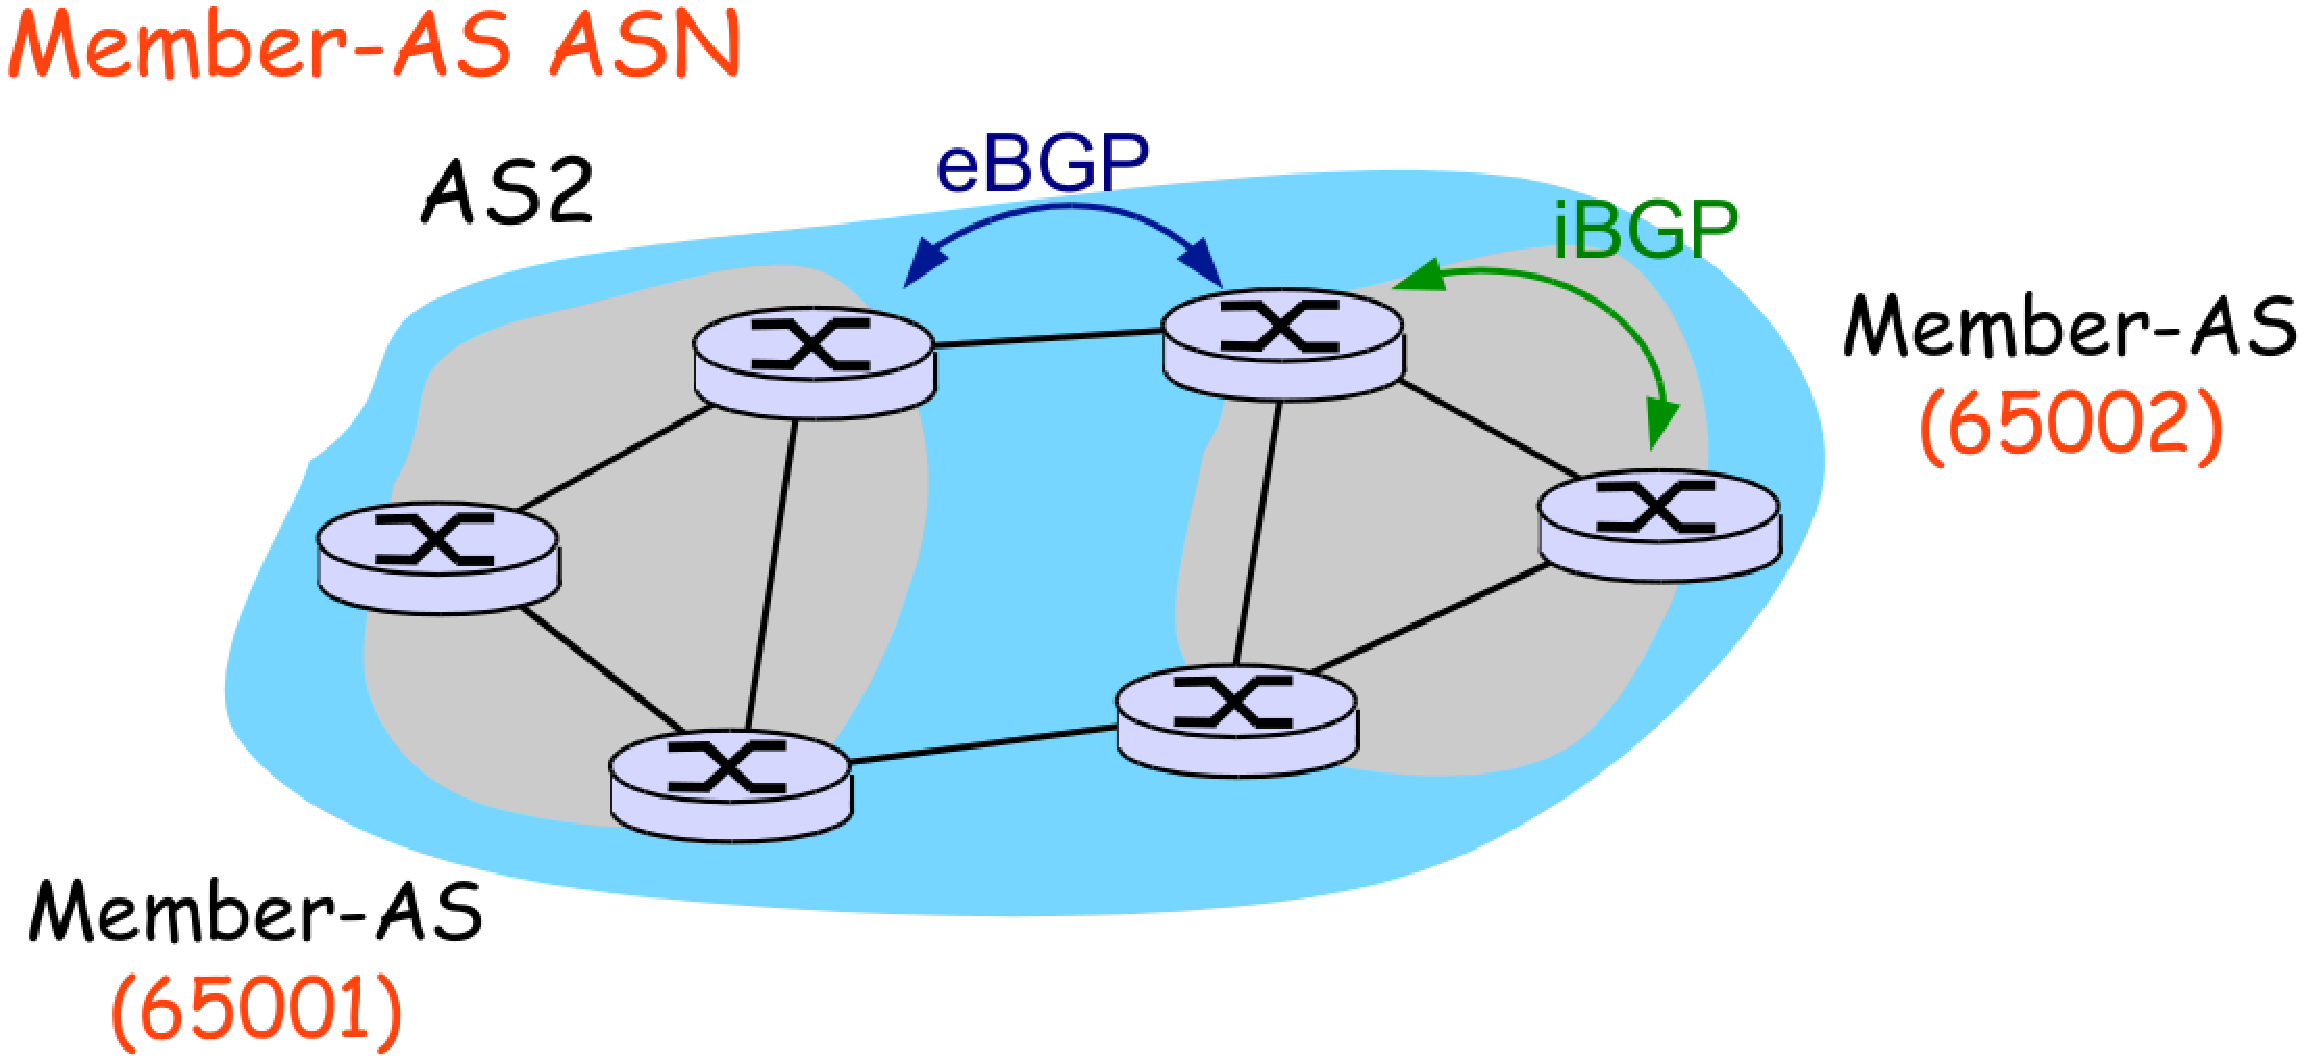
\includegraphics[width=\textwidth]{fab_006.pdf}

\begin{itemize}
\item iBGP est utilisé à l'intérieur de chaque AS-membre, eBGP est
  utilisé entre les AS-membres, chaque routeur a deux ASN: celui de la
  confédération et celui de l'AS-membre.
\item Suivant la session eBGP, un routeur appartient à l'AS-membre ou
  à la confédération.
\item Lors de la propagation d'un UPDATE via eBGP vers un routeur de
  la même confédération, un routeur insert son ASN-membre dans
  l'AS-PATH
\item Il est autorisé d'annoncer un NEXT-HOP inchangé ainsi que
  l'attribut LOCAL-PREF.
\item Lorsque qu'un UPDATE est propagé en dehors de la confédération
  via eBGP, le routeur doit d'abord enlever les ASN-membre et ajouter
  l'ASN de la confédération.
\end{itemize}

\subsection{Réflection de routes}

Des routeurs spéciaux appelés \textbf{réflecteurs de routes} peuvent
propager sur une session iBGP des routes reçues d'une autre session
iBGP.

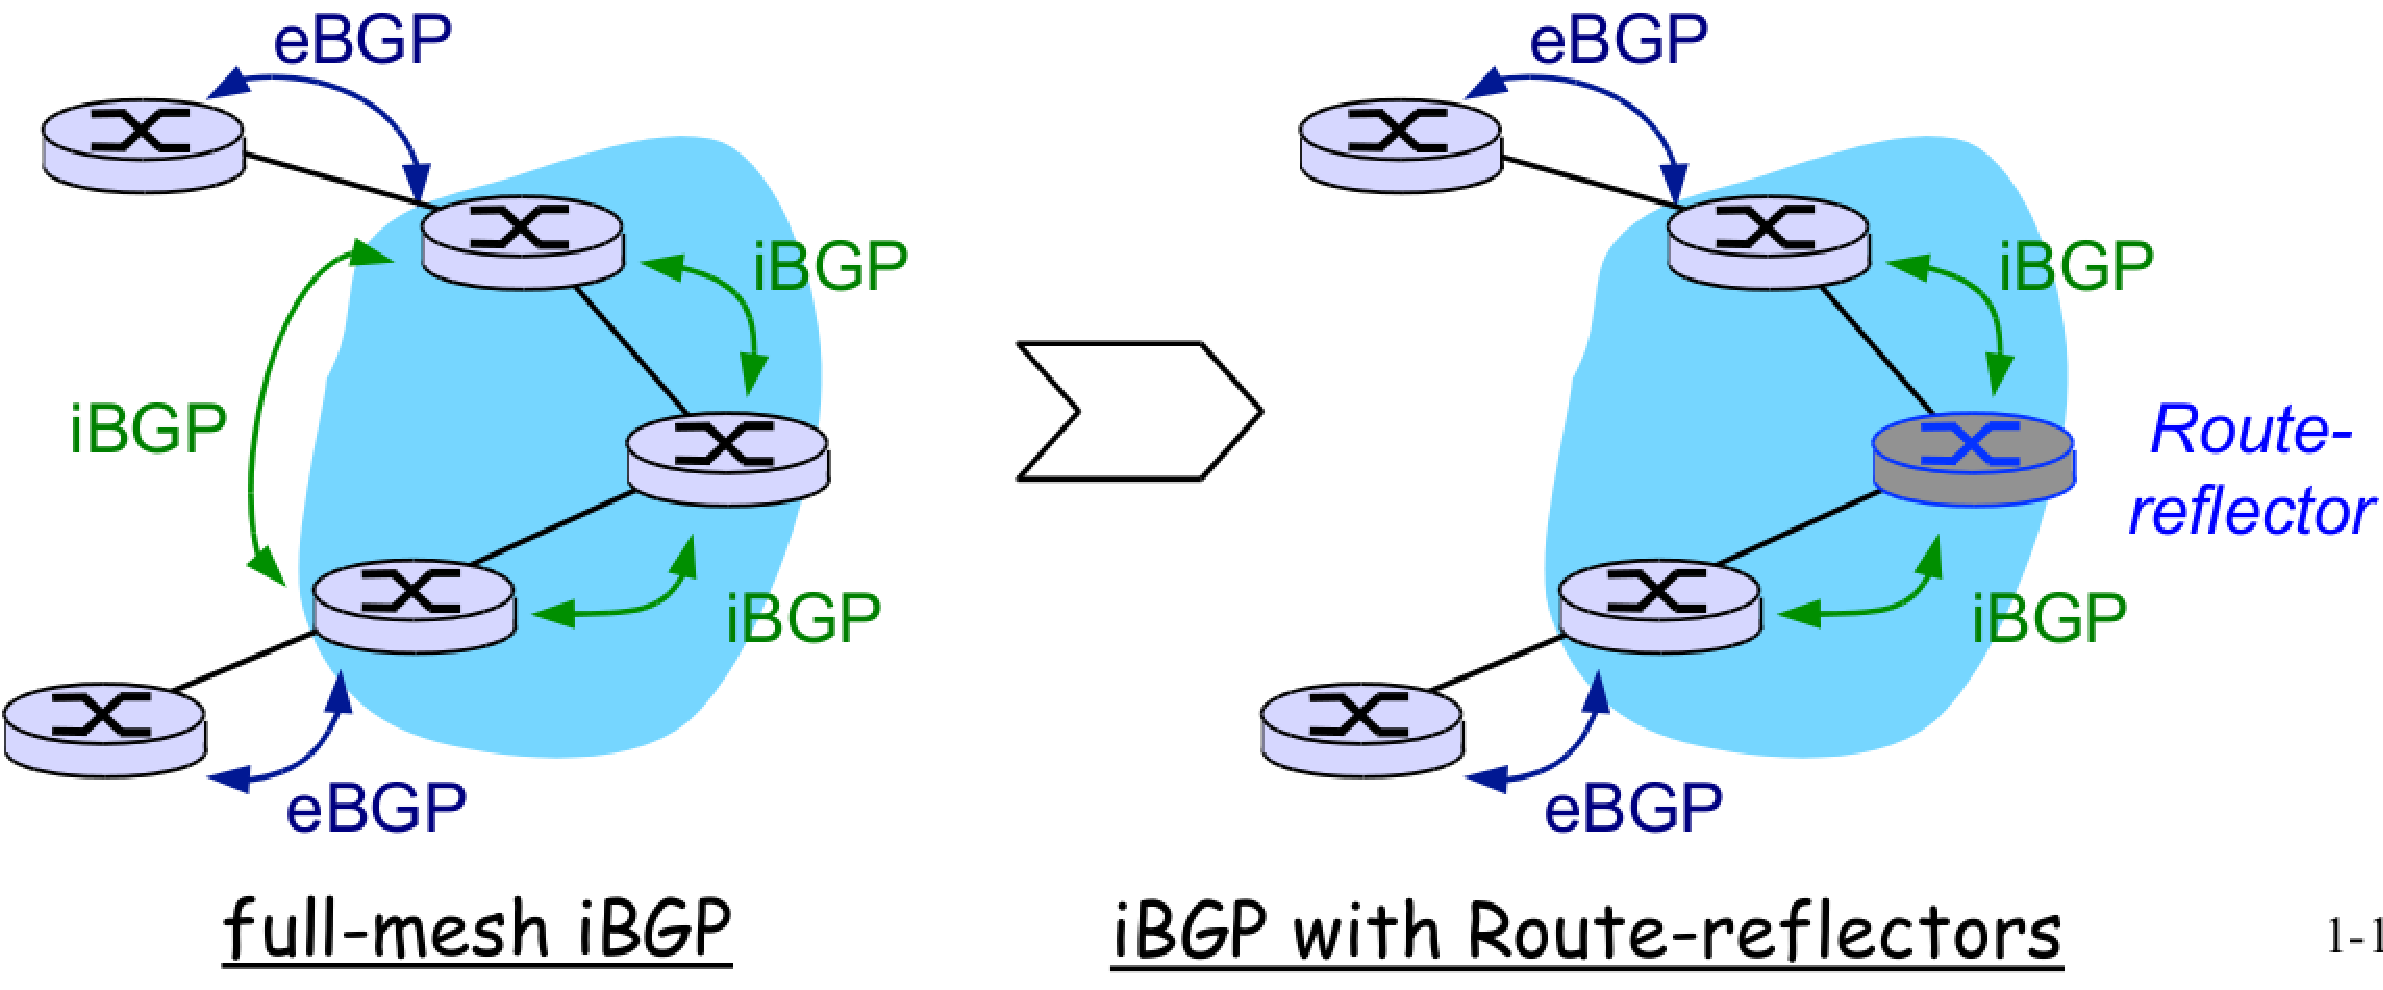
\includegraphics[width=\textwidth]{fab_007.pdf}

Il y a deux types de noeuds iBGP quand il y a des RR: les noeuds
clients qui ne participent pas au full-mesh et les noeuds non-clients,
en full-mesh.

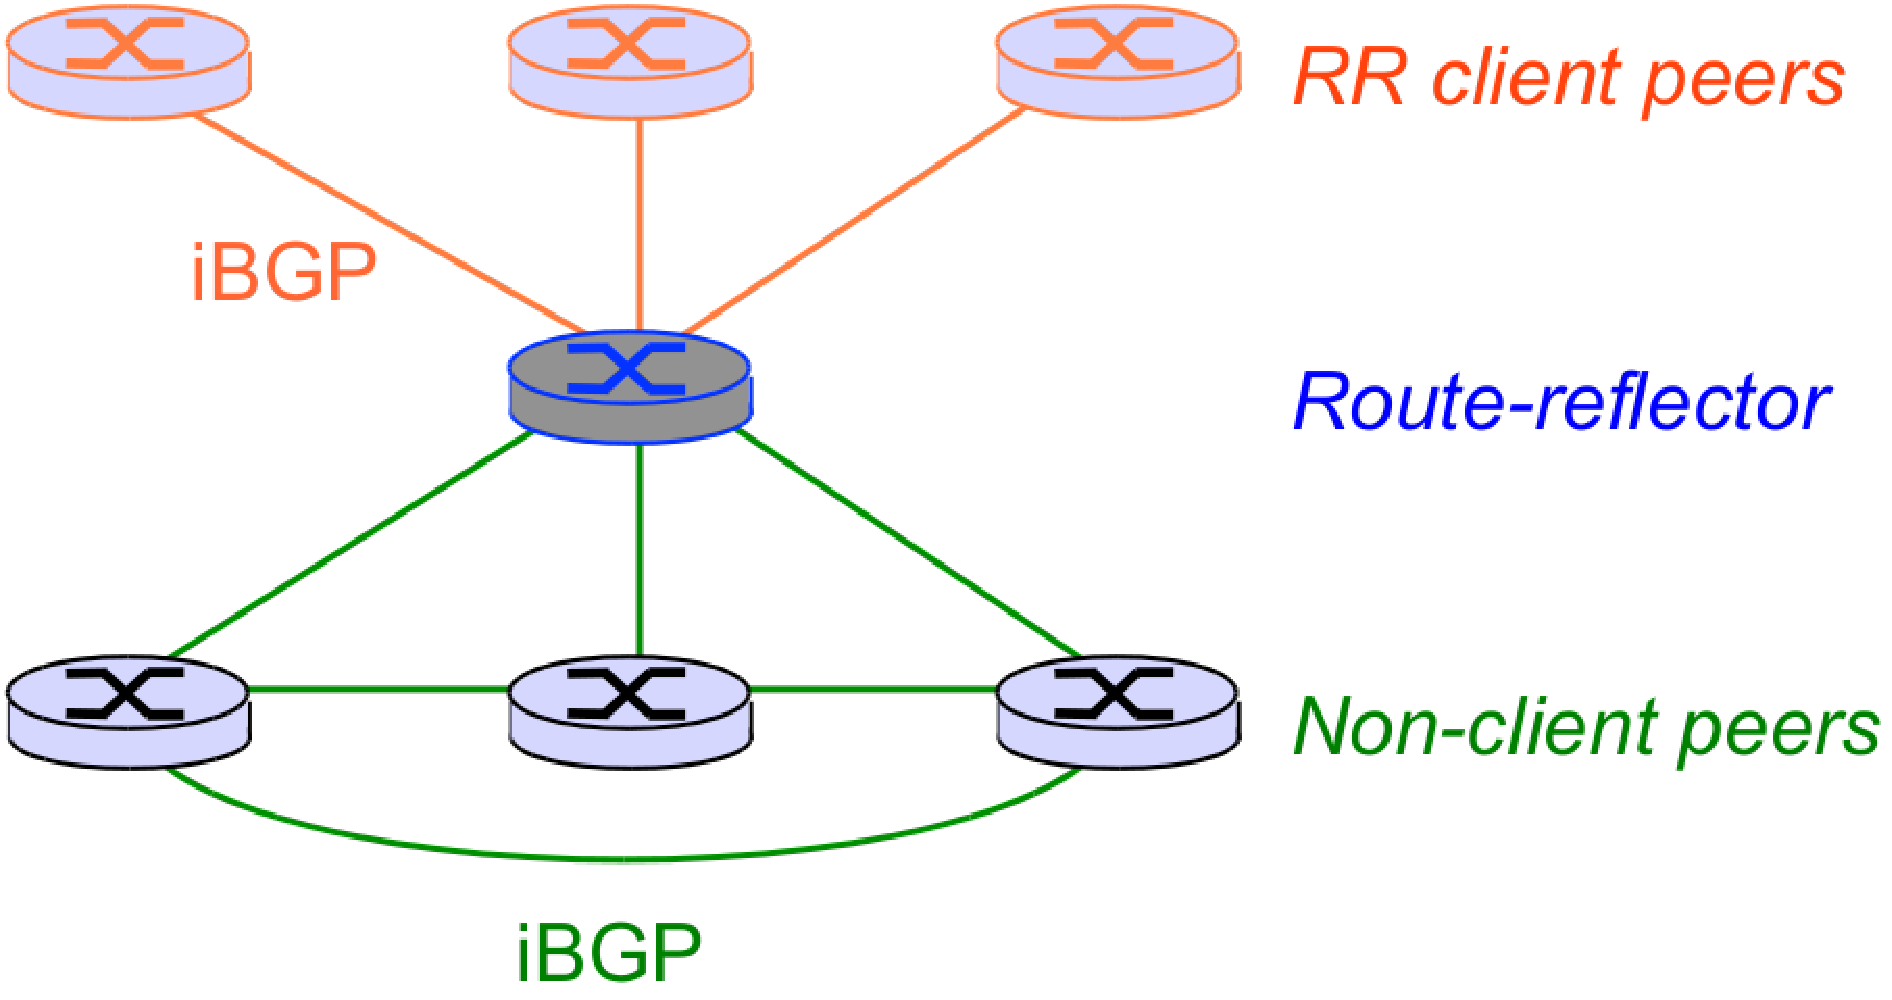
\includegraphics[width=\textwidth]{fab_008.pdf}

Quand un RR reçoit une route d'un client ou de eBGP, il la redistribue
à tout le monde.

Quand un RR reçoit une route d'un non-client, il ne la redistribue
qu'aux clients.

\paragraph{Tolérance aux pannes}

Lorsque le RR tombe en panne, tous les clients sont déconnectés
(single point of failure). Pour éviter cela, chaque client est
connecté à au moins 2 RR.

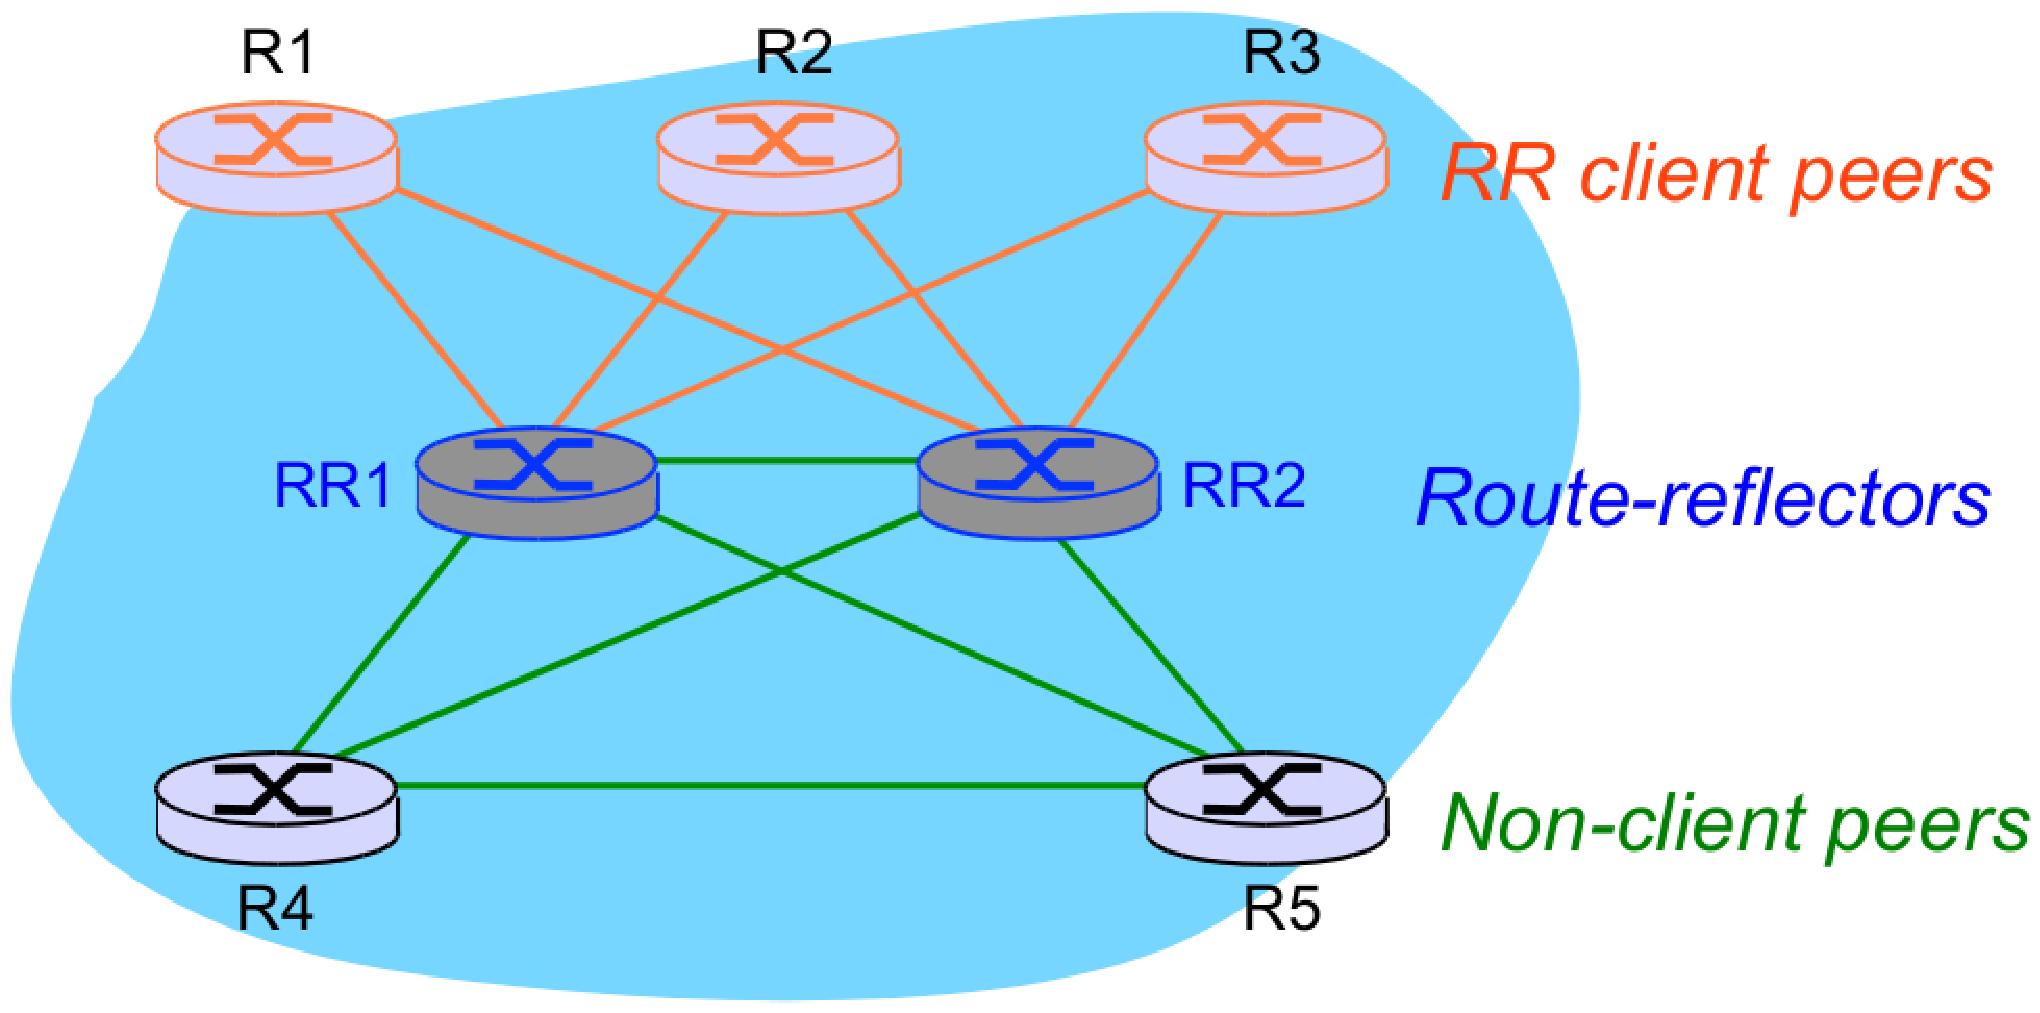
\includegraphics[width=\textwidth]{fab_009.pdf}

\paragraph{Problème: les boucles de routage sont possibles}

Nous devons être sûr qu'un update ne peut être retourné à celui qui
l'a anoncé. Or, avec 2 RR, un client envoie l'UPDATE au premier RR,
qui le transmet au second, qui le renvoie au client (boucle).

La solution à ce problème est l'attribut BGP ORIGINATOR-ID. Quand un
RR réfléchit une route, il place l'identifiant du client qui a
envoyé la route dans l'ORIGINATOR-ID.

Les routeurs se voyant dans l'ORIGINATOR-ID refusent systématiquement
la route.

\paragraph{Hiérarchies de RR}

Un RR peut être lui-même client d'un autre RR, les mêmes règles de
redistribution des routes s'appliquent.

S'assurer que les boucles de routage sont impossibles devient moins
simple, ORIGINATOR-ID ne résoud plus ce problème.

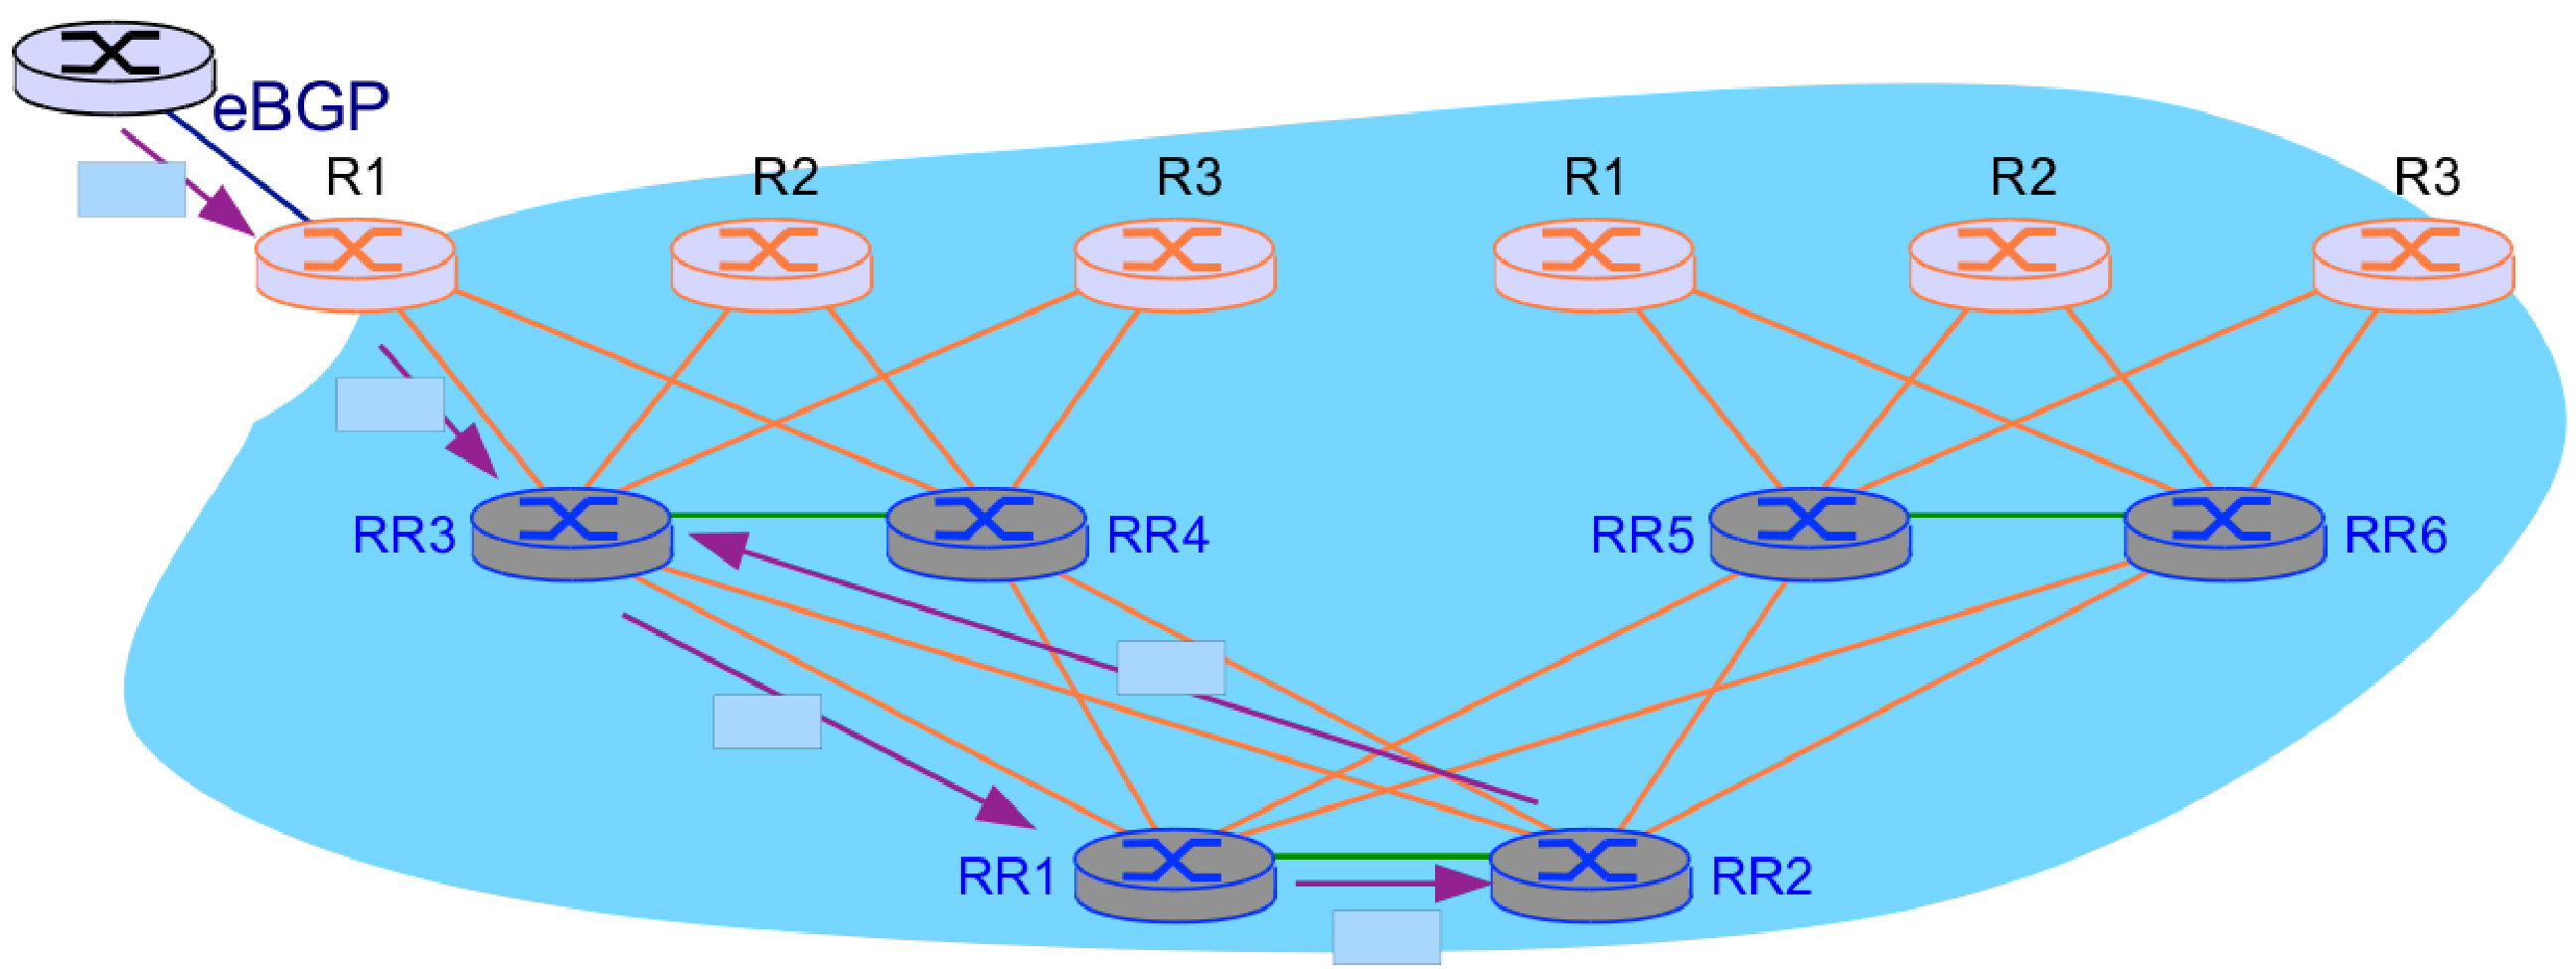
\includegraphics[width=\textwidth]{fab_010.pdf}

Comme réponse à ce problème, on introduit un nouvel attribut:
CLUSTER-ID-LIST; quand un RR réfléchit une route, il ajoute son propre
identifiant de cluster à la liste de la route.

Ensuite, pour éviter les boucles de routage, il suffit d'empêcher les
routes d'atteindre un cluster par lequel elle est déjà passée.

\paragraph{Processus de décision, règles 9 et 10}

On comprend à présent les tie-breaks 9 et 10 du processus de décision;
l'ORIGINATOR-ID et la CLUSTER-LIST proviennent en fait des clusters
lorsqu'on utilise les réflecteurs de routes.

\paragraph{Comparaison entre les RR et les confédérations}

Avec les RR, les clients ne doivent pas être au courant de la
hiérarchie, il suffit de configurer les RR, mais en contrepartie, la
charge de travail est très forte sur les RR, qu'on installe en général
sur les routeurs les plus puissants.

Avec les confédérations, il est simple de migrer d'une topologie
multi-AS vers une simple confédération (par exemple, lorsqu'une
société rachète une autre, elle peut vouloir intégrer le réseau de la
société achetée au sien avec le moins de coûts possible). Le point
noir des confédérations est que chaque routeur doit être configuré
pour connaître l'id de sa confédération et de son AS-membre.

\subsection{Filtres à grande échelle: les communautés}

Une communauté est une valeur entière spéciale qu'on peut attacher à
une route, elle est encodée sur 32 bits et deux routes avec la même
communauté attachée sont générallement traitées de la même manière.

Certaines valeurs de communauté sont standardisées, par exemple
$0xFFFFFF01$ (NO\_EXPORT) et $0xFFFFFF02$ (NO\_ADVERTISE).

Chaque AS dispose de 65536 valeurs de communautés pour lesquelles il
peut définir la sémantique qu'il souhaite (ASN:0000 $\rightarrow$
ASN:FFFF)

La valeur d'attribut BGP COMMUNITY contient une ensemble de valeurs de
communautés.

\paragraph{Exemple d'utilisation des communautés}

Souvent, les AS utilisent les communautés comme ceci: chaque routeur
en relation avec un client applique un filtre à toute les routes
reçues dont l'action est d'ajouter une communauté dont la valeur
signifie ``client'', de même pour les routeurs en relation avec des
pairs (valeur ``pair'') et les fournisseurs (valeur ``fournisseur'')

Ensuite, la politique peut être appliquée en fonction des communautés
plutôt qu'en fonction des routeurs, ce qui simplifie générallement le
travail des administrateurs réseaux.

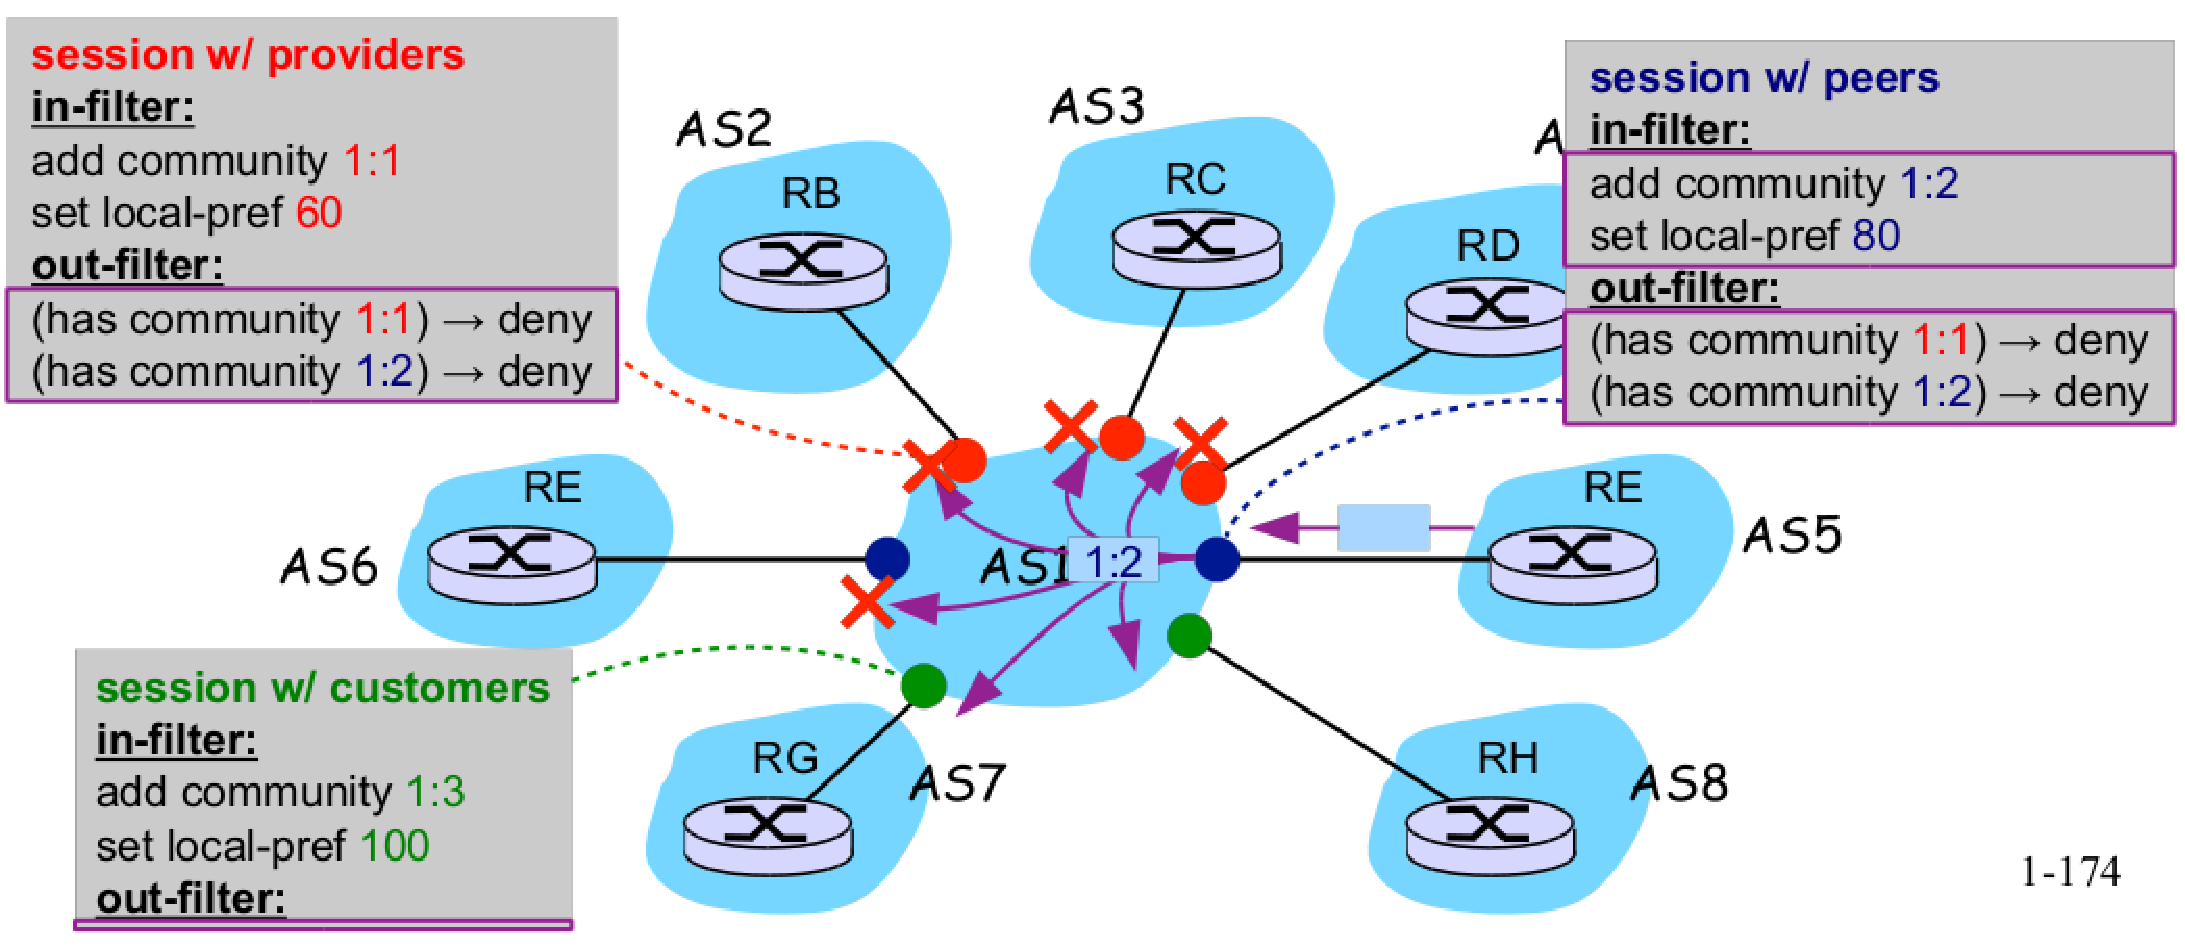
\includegraphics[width=\textwidth]{fab_011.pdf}

\paragraph{Exemple plus complexe: ISP de recherche fournissant 2 types de
  services}

Les universités ont accès au réseau de recherche, les universités et
les institutions gouvernementales ont accès à l'internet commercial.

Pour mettre cela en place, il suffit de ``tagger'' les routes (avec
des communautés) apprises depuis des destinations de recherche ou
commerciales. Ensuite il ne faut annoncer que les universités qu'au
réseau de recherche et le réseau de recherche qu'aux universités.

\paragraph{ISP commercial fournissant 2 services de transit}

Le transit ``plein'' (annoncer toutes les routes connues aux clients,
et les routes des clients aux autres clients, aux pairs et aux
fournisseurs) et des routes clientes uniquement (n'annoncer à ces
clients que les routes apprises par d'autres clients, n'annoncer les
routes apprises par ce client qu'aux autres clients)

\paragraph{Autres utilisations}

On peut utiliser les communautés pour tagger la provenance des routes
(pays), le point d'interconnexion d'où a été reçue la route, etc.

Une fois que les communautés sont apposées sur les routes, on peut les
utiliser comme bon nous semble, par exemple faire des annonces
sélectives sur bases des communautés, de l'AS-PATH prepending, etc.

\paragraph{Inconvénients}

Les communautés sont un attribut transitif. Dans certains cas c'est un
atout, différents AS peuvent ainsi collaborer, mais en général ça
donne surtout des routes polluées par un nombre parfois impressionnant
de communautés, inutiles, mais les routeurs doivent quand même
regarder ces communautés (consommation, mémoire, ...) et générallement
les communautés ont une sémantique locale uniquement.

La meilleure chose à faire pour un routeur qui utilise les
communautés, c'est de s'assurer que ces dernières ne sont pas
annoncées inutilement à l'ensemble de l'internet.

\subsection{Stabilité}

\subsection{Nombre de messages échangés}

Bien que BGP soit un protocole incrémental, il n'en reste pas moins
très bavard, pour plusieurs raisons:

\begin{itemize}
\item Les réseaux apparaissent et disparaissent
\item Il y a toujours un routeur qui redémarre quelque part
\item Disfonctionnements matériels, lignes arrachées, carte réseau qui
  ``flappe'', ...
\item Mauvaise configuration
\item Exploration du chemin (plusieurs itérations nécessaires avant de
  trouver la meilleure route)
\item Bugs logiciels
\item Instabilité IGP exportée à l'extérieur de l'AS (tie-break IGP et
  règle ``NEXT-HOP le plus proche feront qu'un routeur pourrait
  changer de meilleure route sans arrêt)
\item Algorithmes de routage secrets tentant des astuces suspectes ...
\item Interactions politiques louches
\item Gnomes, étincelles, fées, etc.
\end{itemize}

\paragraph{Comment réduire le nombre de messages UPDATE ?}

Le MRAI (Minimum Route Advertisement Interval) peut être augmenté
(réduit le nombre de messages mais peut allonger le temps de
convergence de BGP)

La plupart des routes ne changent pas fréquemment, une petite part des
routes sont responsables de la plupart des messages BGP échangés. On
peut associer un compteur pénalisant à chaque route, l'incrémenter
chaque fois qu'une route change et utiliser un délai exponentiel pour
lentement diminuer le compteur sur la durée.

Les routes avec un compteur trop élevé sont alors simplement
supprimées pour un certain temps.

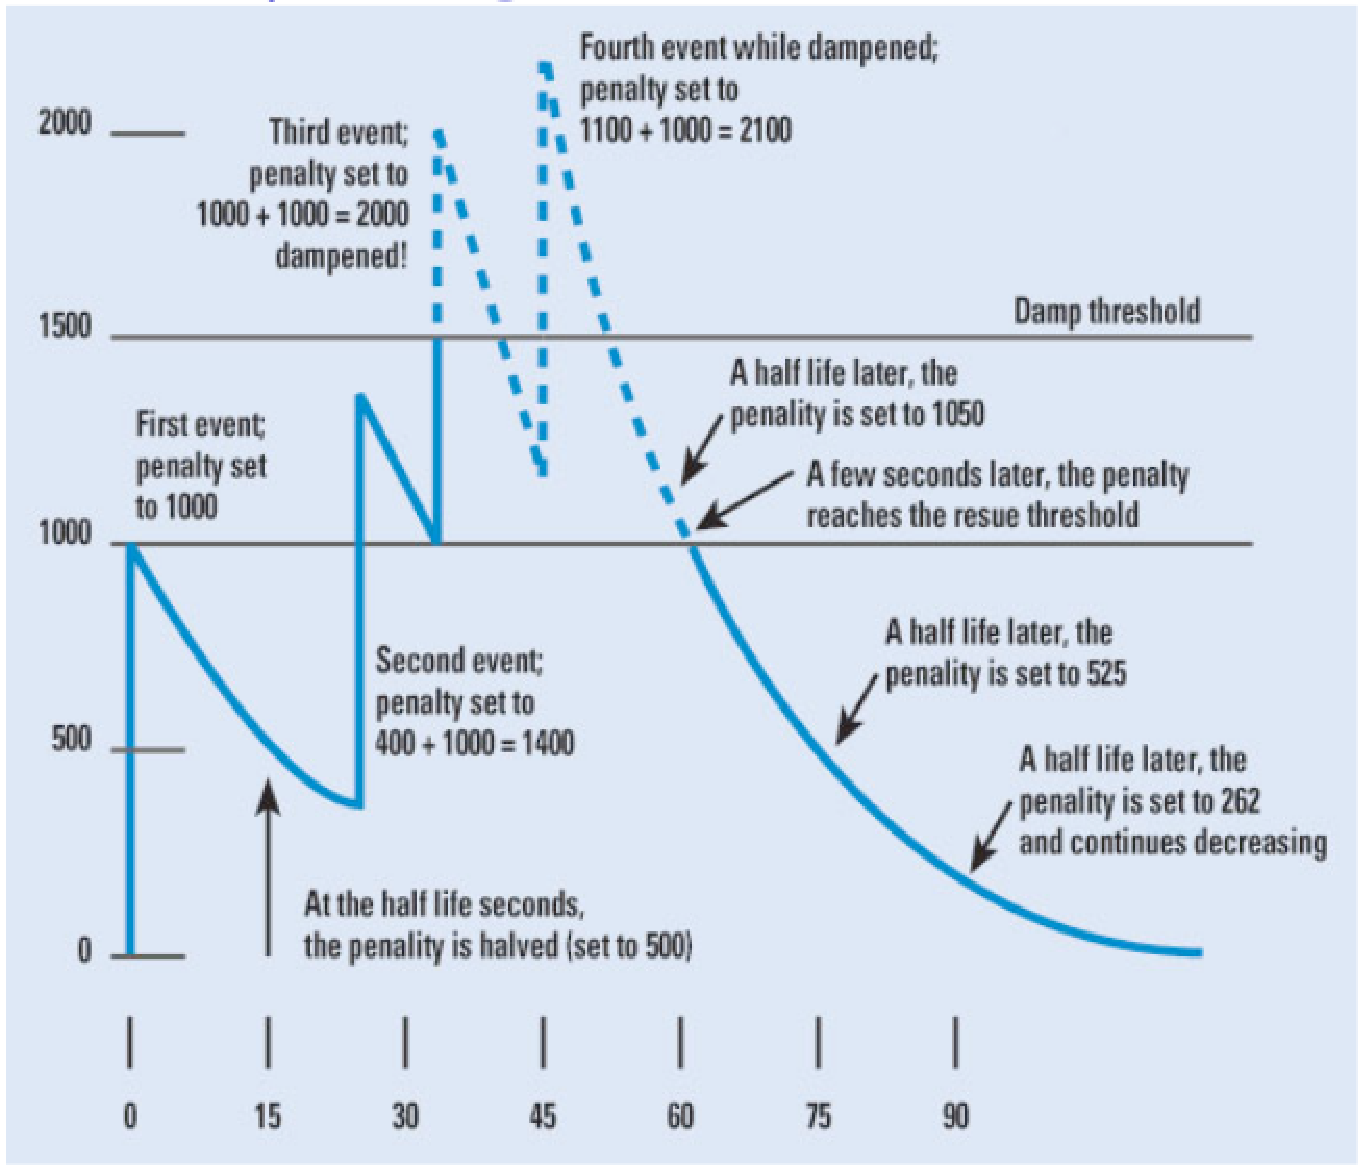
\includegraphics[width=\textwidth]{fab_012.pdf}

L'utilisation de cette technique (BGP dampening) est découragée
aujourd'hui, car elle peut avoir un effet néfaste en diminuant la
convergence pour des préfixes valides mais qui doivent faire une
exploration du chemin avant de trouver leur meilleure valeur.

\subsubsection{Stable Path Problem (SPP)}

Raisonner quant à la conformité d'un système BGP est un problème
toujours ouvert aujourd'hui.

Le système a-t-il une solution ? Combien de temps durera la
convergence ?

Le SPP est une première tentative pour formaliser la manière dont BGP
fonctionne.

Un SPP est composé d'un graphe $G=(V, E)$, $V = \{0,1,2,\dots\}$,
$peers(u)=\{w|\{u,w\} \in E\}$, par convention, $0$ est le noeud
origine.

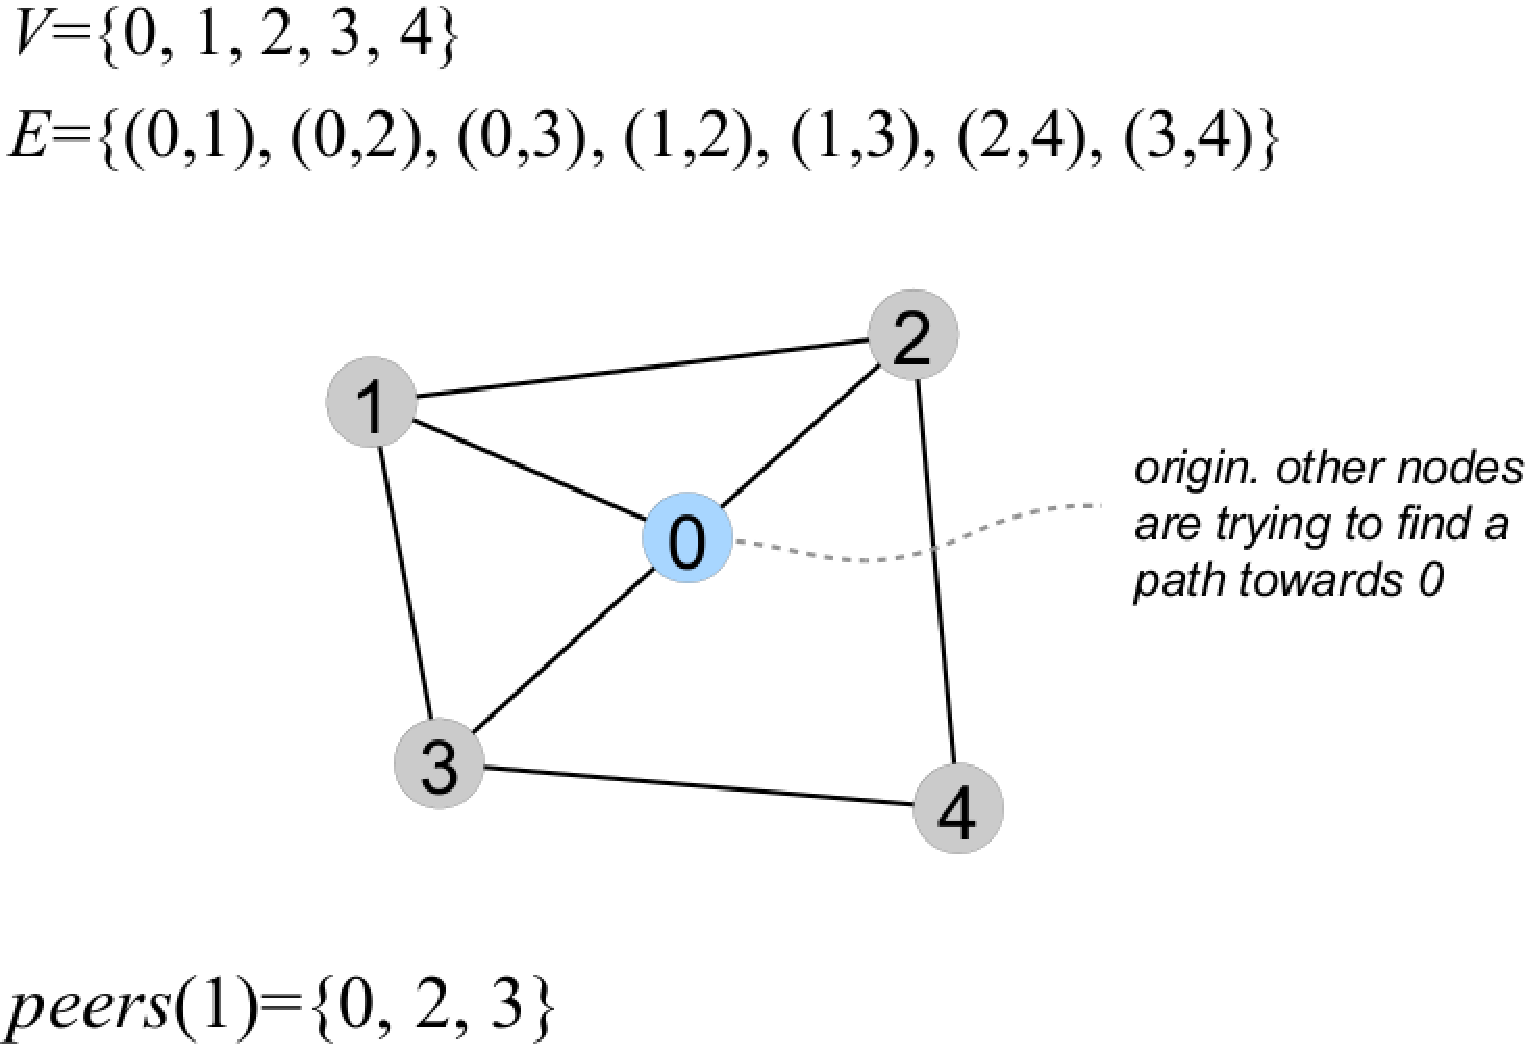
\includegraphics[width=\textwidth]{fab_013.pdf}

Un chemin est une séquence $v_k, v_{k-1}, \dots, v_0$de noeuds telle
que chaque paire successive dans la séquence forme un arc dee $V$. Le
chemin vide est désigné par $\epsilon$. Chaque chemin non vide a une
direction de son premier noeud $v_k$ vers son dernier noeud $v_0$.

Pour chaque noeud $v$, $P^v$ désigne l'ensemble des chemins permis de
$v$ à $0$.

Si $P = (v, v_k, \dots, v_0) \in P^v$ , $v_k$ est appelé NEXT-HOP du
chemin $P$.

$P^*$ est l'union de tous les $P^v$

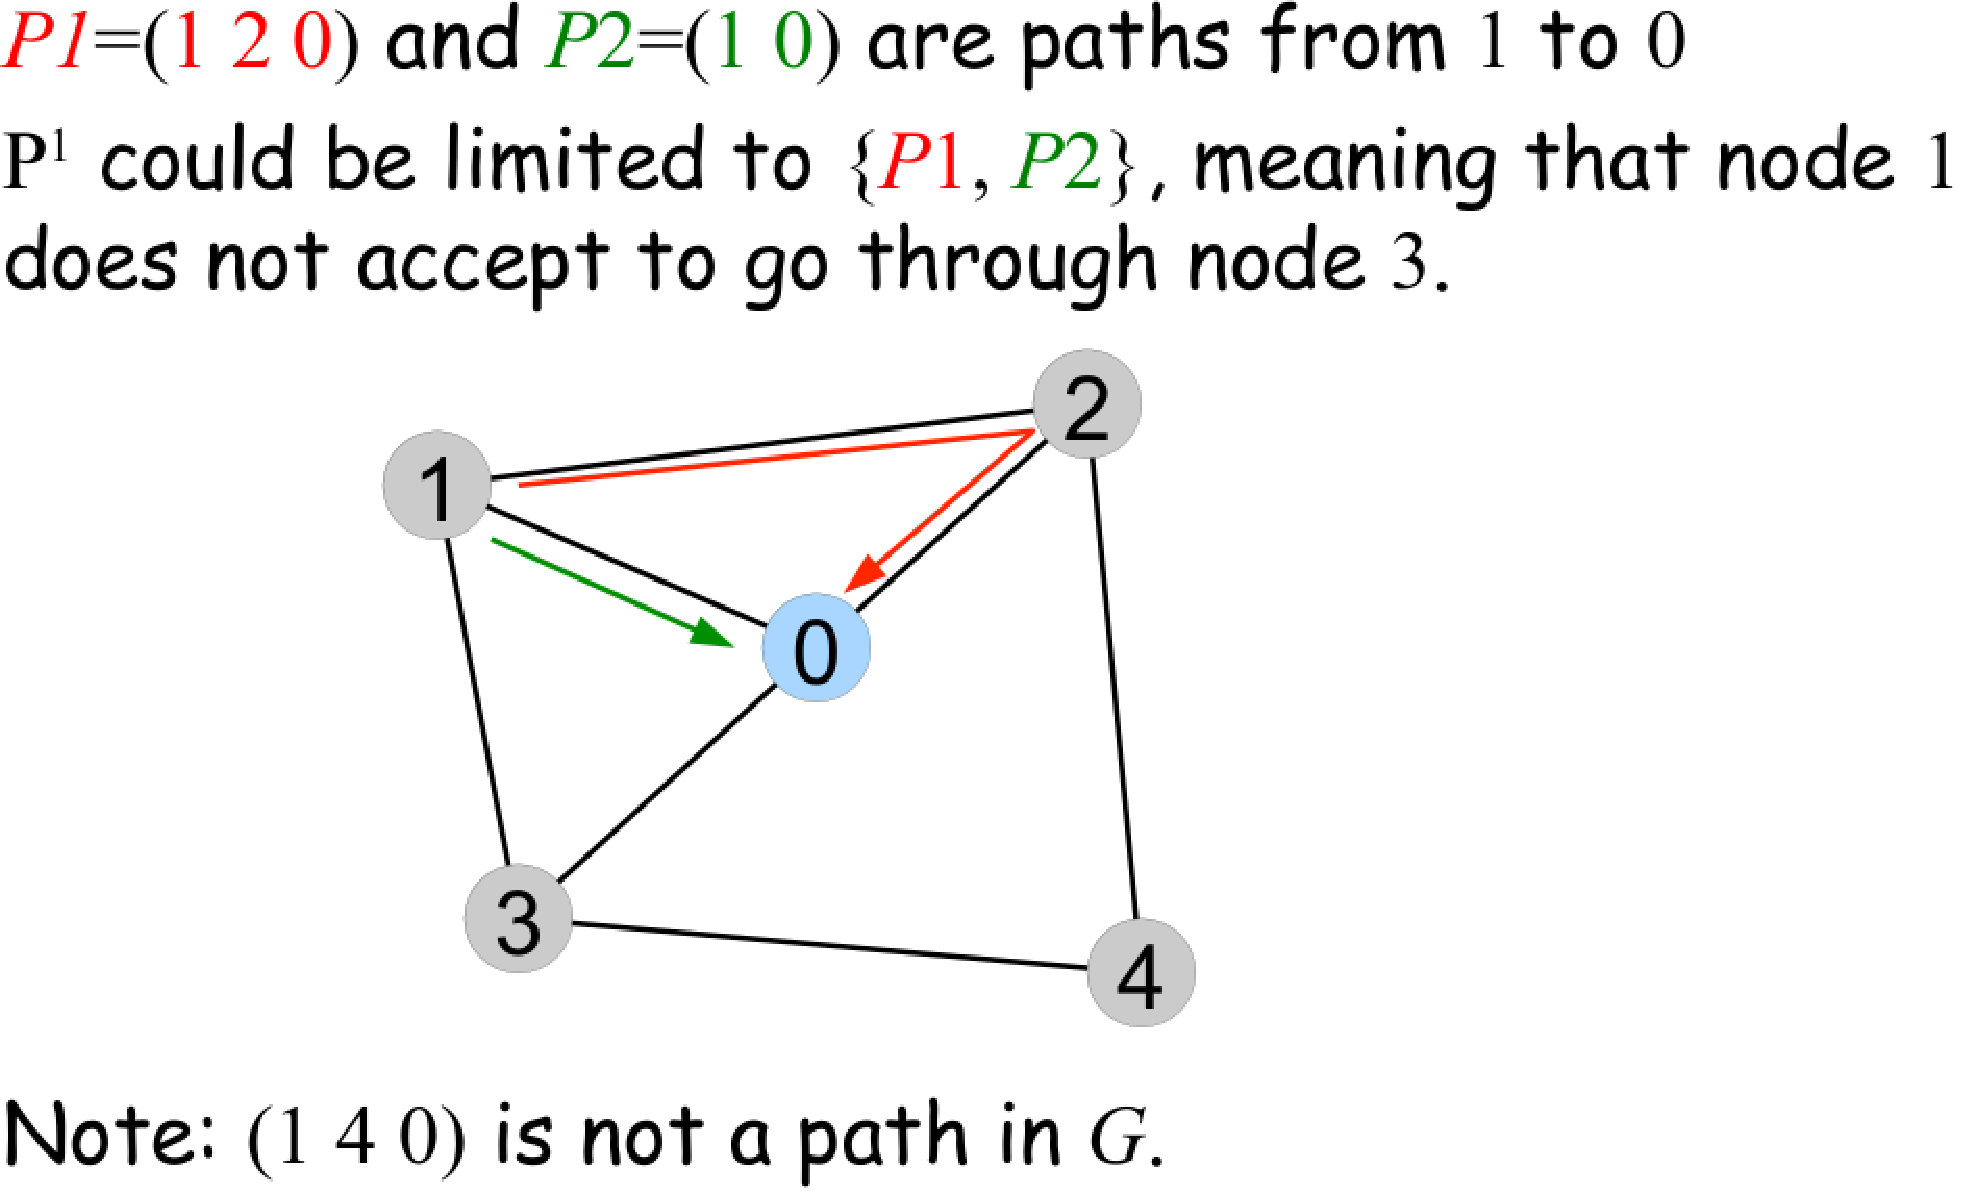
\includegraphics[width=\textwidth]{fab_014.pdf}

Le rang d'un chemin pour un noeud $v$ est une fonction $\lambda^v :
P^v \rightarrow R^+$ qui represente comment $v$ range ses chemins
permis.

Si $P1, P2, P^v$ et $\lambda^v(P1) < \lambda^v(P2)$, alors $P2$ est
dit préféré à $P1$.

$\Lambda = \{\lambda^v | v \in V-\{0\}\}$

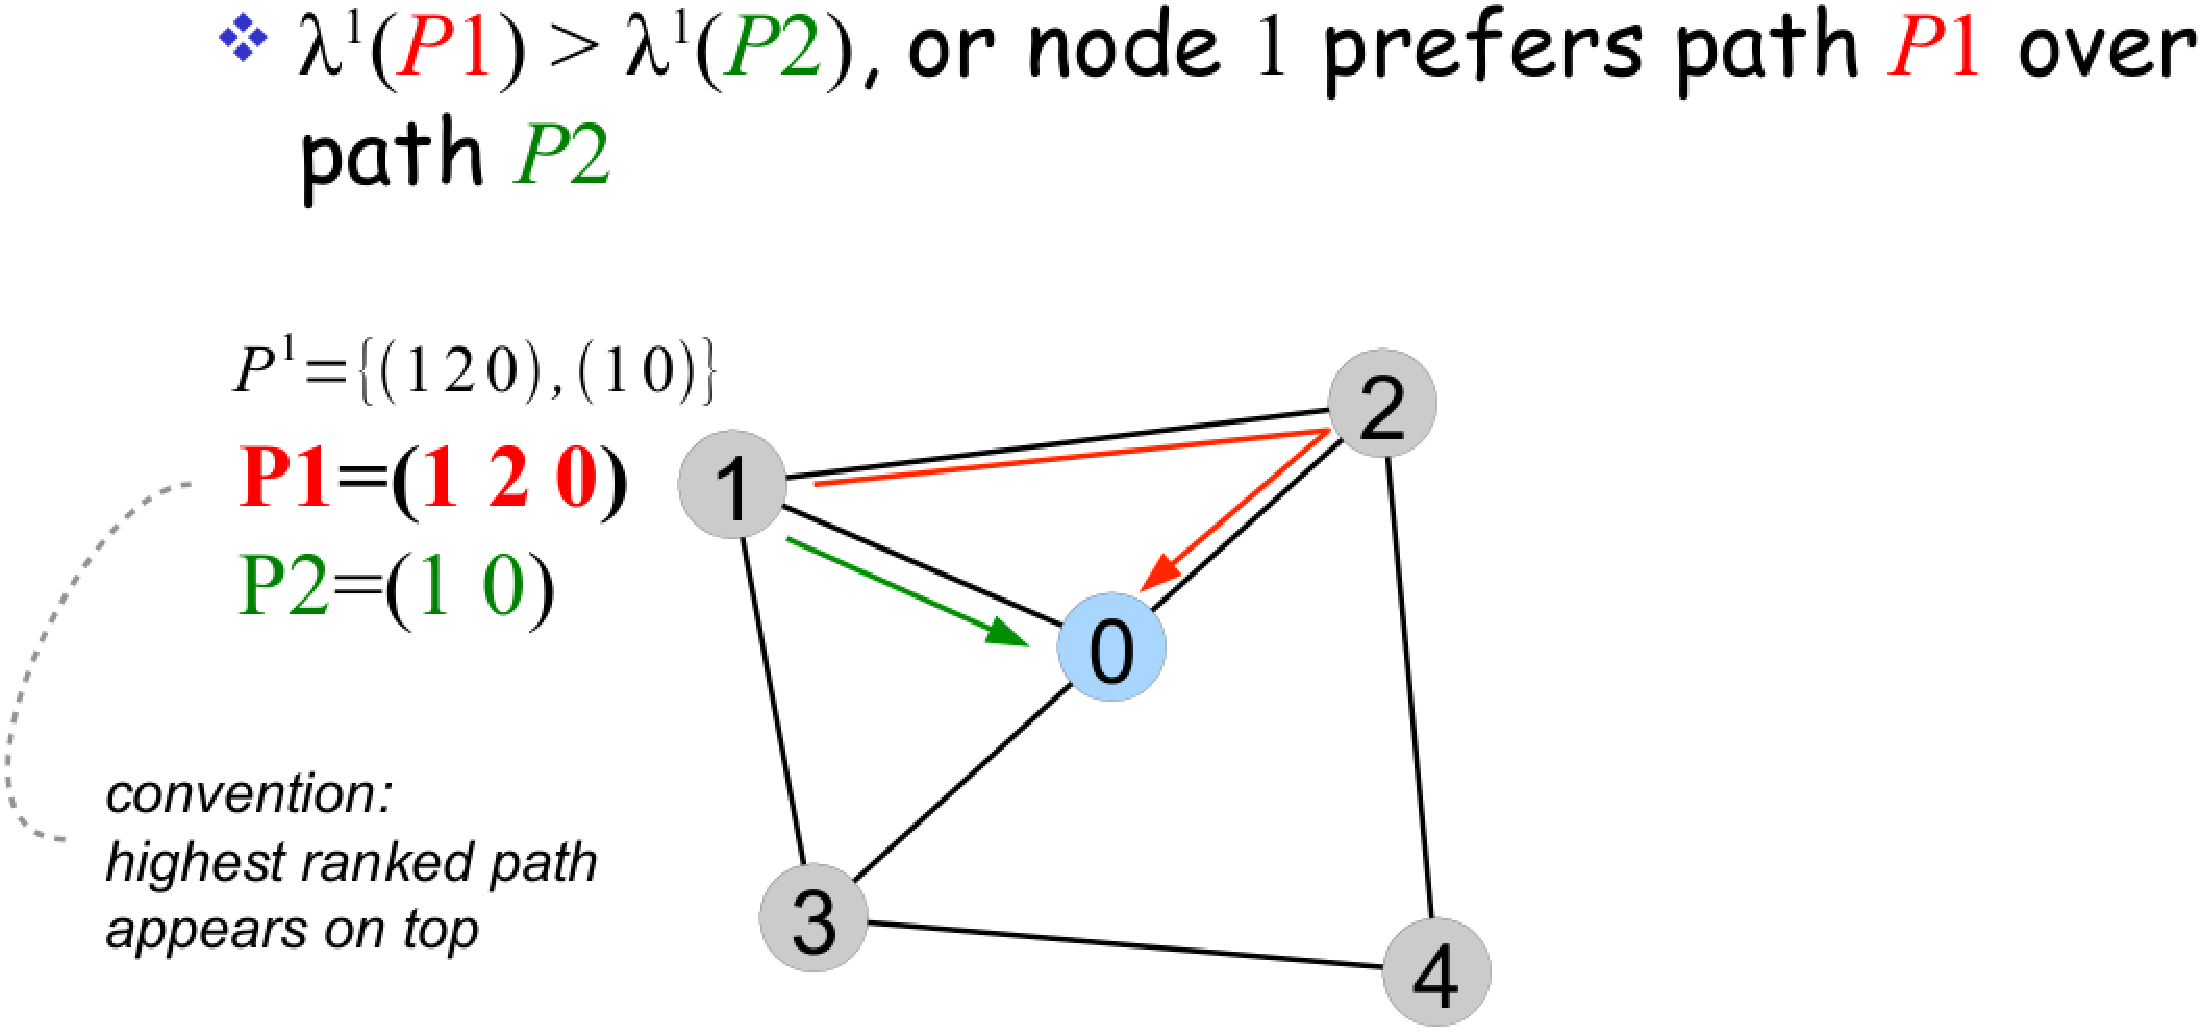
\includegraphics[width=\textwidth]{fab_015.pdf}

Une instance SPP $S = (G, P^*, \Lambda)$ admet $P^0=\{(0)\}$.

$\pi(v)$ représente une assigation de chemin pour $v$. Si la valeur
est $\epsilon$, on considère qu'aucun chemin ne lie $v$ à $0$ dans
l'assignation courante.

$choices(\pi, v)$ représente les chemins possibles, via l'assignation
courante, que $v$ a pour atteindre $0$.

Le meilleur chemin P dans l'ensemble $W$ pour un noeud $u$, noté
$best(W, u)$ est tel que $\lambda^u(P)$ est plus grand que tout autre
chemin de $W$.

Une assignation $\pi$ est stable en $u$ si $\pi(u) = best(choices(\pi,
u), u)$ qui signifie que $u$ est assigné au meilleur de ses choix.

Une assignation est stable si elle est stable en chacun de ses noeuds.

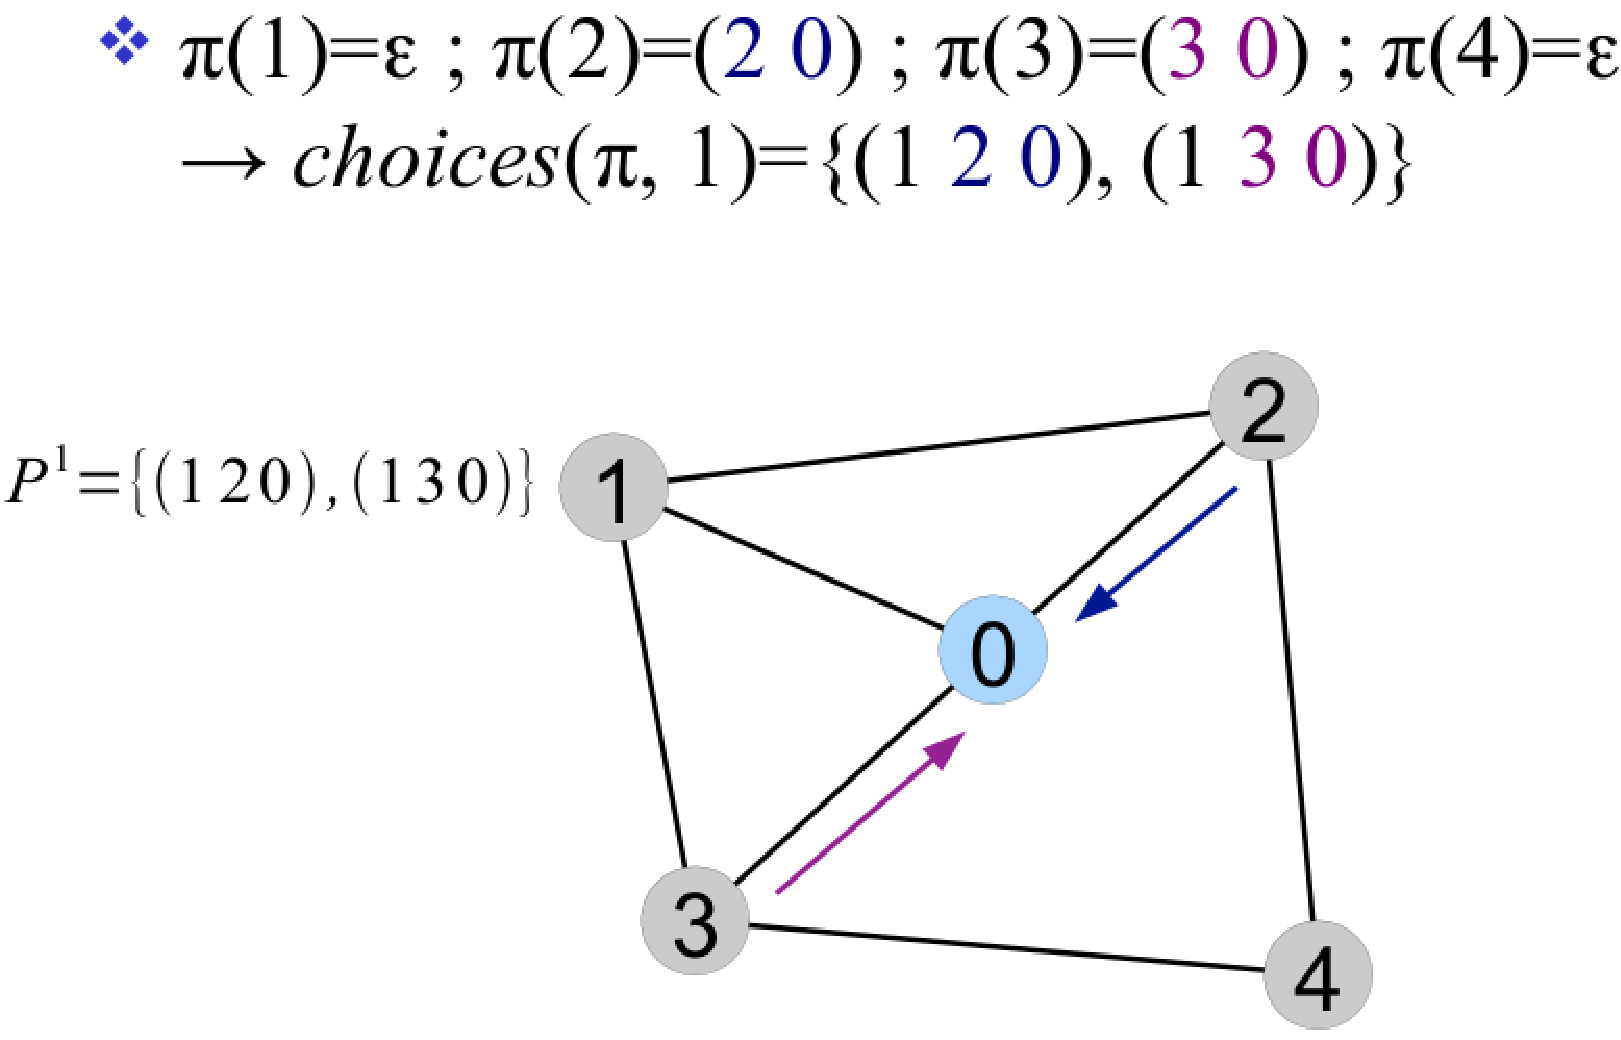
\includegraphics[width=\textwidth]{fab_016.pdf}

Une instance SPP est solvable si une assignation stable existe pour
l'intance, on appelle cette assignation la solution de l'instance;
sinon l'instance est dite insolvable.

Une méthode pour trouver les assignements possibles, ainsi que les
solutions, est de faire un tri topologique sur le graphe de
dépendances, et ensuite d'ajouter les noeuds, dans cet ordre, jusqu'à
ce que tous les noeuds soient ajoutés, on voit alors toutes les
possibilités, pour choisir celles qui sont des solutions, il suffit de
regarder qu'à chaque noeud de l'arbre ainsi construit, la branche est
bien le meilleur choix.

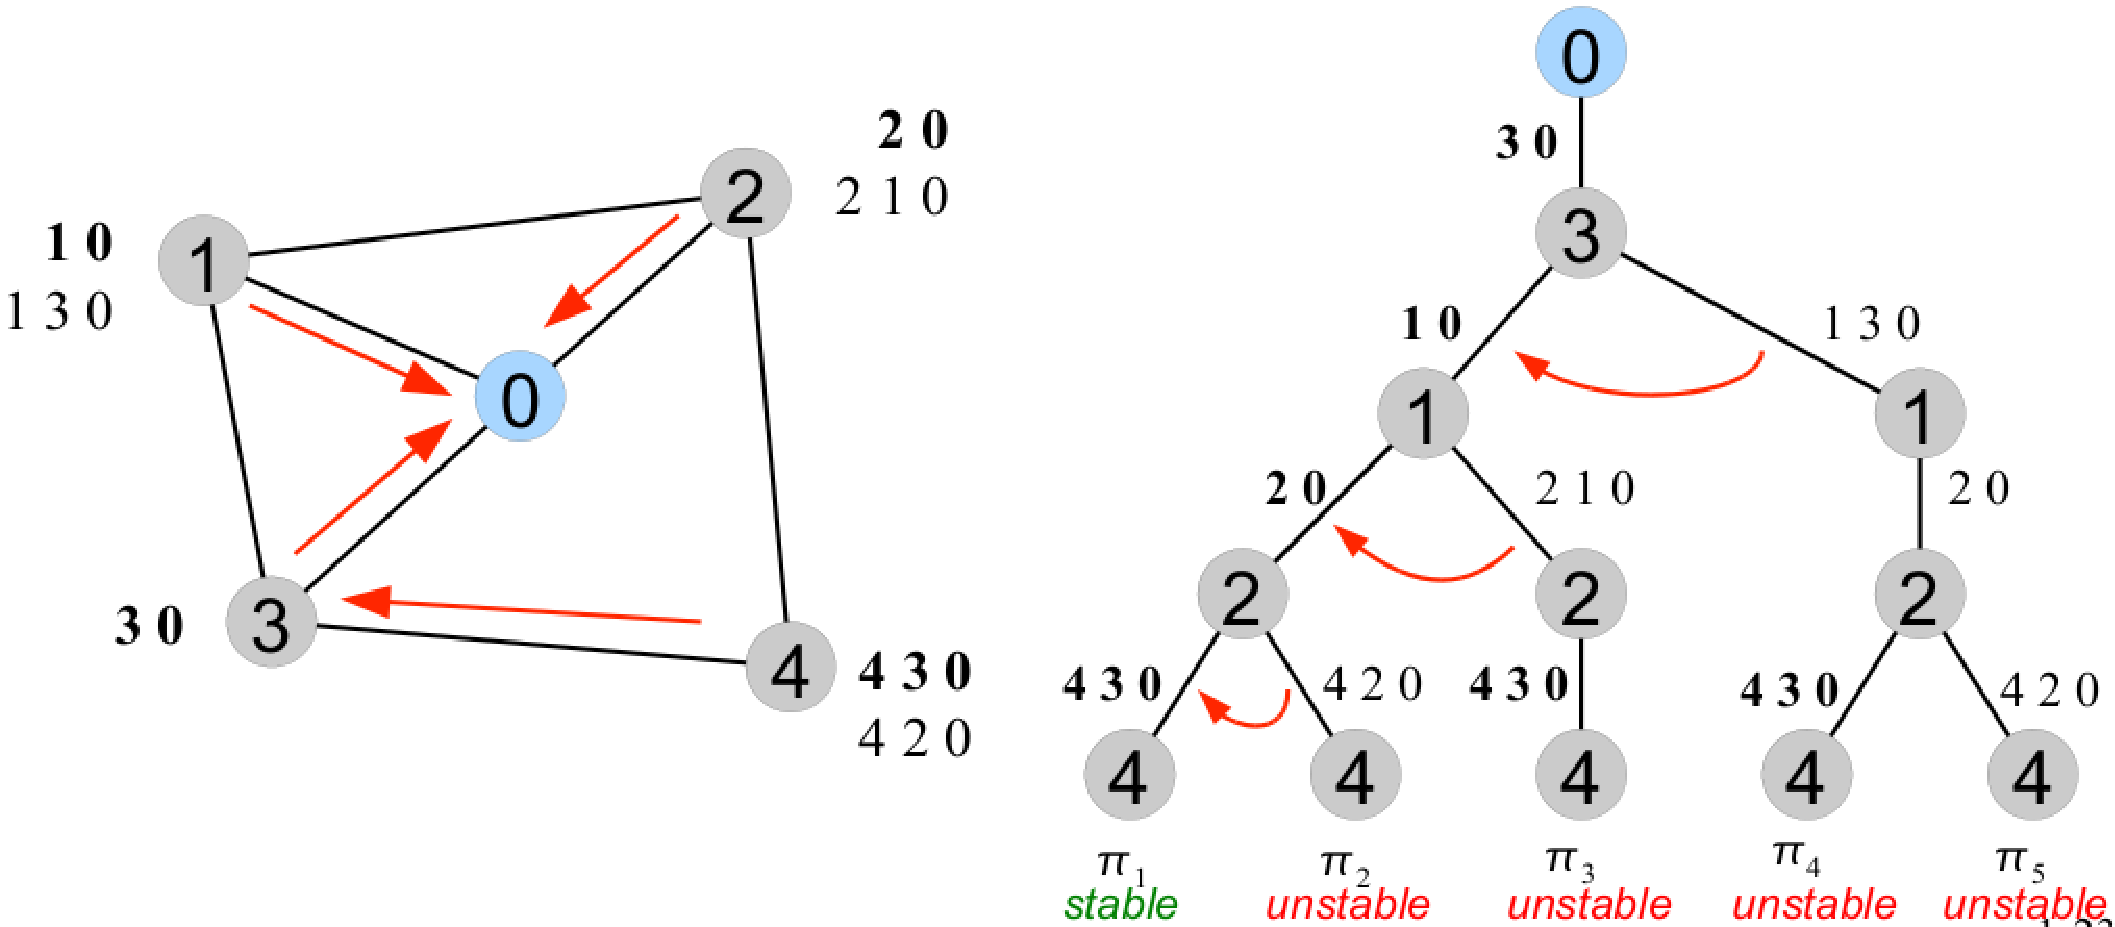
\includegraphics[width=\textwidth]{fab_017.pdf}

Dans cet exemple, la solution est un shortest-path tree, ce n'est pas
toujours le cas. Cette méthode se base sur le fait que le graphe de
dépendances est un DAG, ce n'est pas une condition nécessaire pour que
l'instance ait une solution. (Exemple: DISAGREE, dont le graphe de
dépendances est ci-dessous)

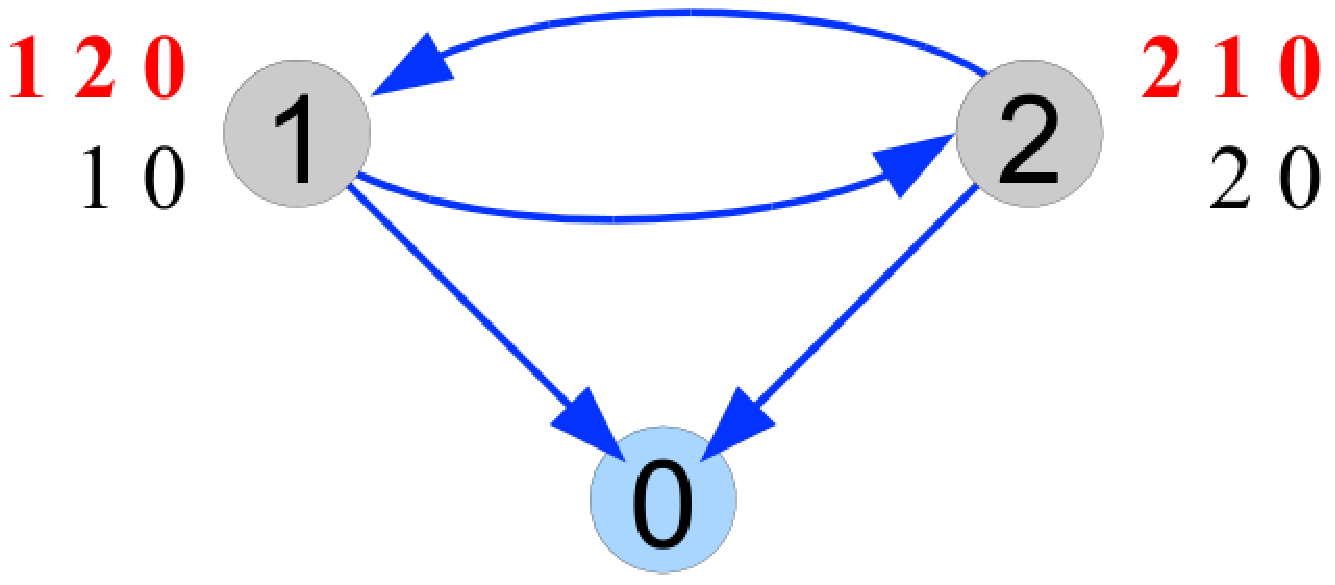
\includegraphics[width=0.5\textwidth]{fab_018.pdf}

\paragraph{Séquence d'activation}

Considérons maintenant le même modèle légèrement modifié, c'est-à-dire
que chaque noeud est indépendant et voit une partie limitée du
réseau. À chaque nouveau ``temps'', un noeud reçoit l'information d'un
voisin, la traite et choisit une nouvelle meilleure route. L'ordre
dans lequel les noeud s'activent est la séquence d'activation.

Exemple de séquence d'activation avec DISAGREE:

\begin{tabular}{|c|c|c|c|}
  \hline
  Step & Event & Noeud 1 & Noeud 2 \\
  \hline
  0 & $(0, 1): \pi(0) = (0)$ & choices=\{(1 0)\} & \\
  & & best=(1 0) & \\
  \hline
  1 & $(1, 2): \pi(1) = (1 0)$ & & choices=\{(2 1 0)\} \\
  & & & best=(2 1 0) \\
  \hline
  2 & $(0, 2): \pi(0) = (0)$ & & choices=\{(2 1 0), (2 0)\} \\
  & & & best=(2 1 0) \\
  \hline
  3 & $(2, 1): \pi(2) = (2 1 0)$ & choices=\{(1 0)\} & \\
  & & best=(1 0) & \\
  \hline
\end{tabular}

On obtient dans ce cas une assignation stable, voici un autre exemple
où les choses se passent moins bien:

\begin{tabular}{|c|c|c|c|}
  \hline
  0 & $(0, 1): \pi(0) = (0)$ & choices=\{(1 0)\} & \\
  & & best=(1 0) & \\
  \hline
  1 & $(0, 2): \pi(0) = (0)$ & & choices=\{(2 0)\} \\
  & & & best=(2 0) \\
  \hline
  2 & $(1, 2): \pi(1) = (1\ 0)$ & & choices=\{(2 0), (2 1 0)\} \\
  & & & best=(2 1 0) \\
  \hline
  3 & $(2, 1): \pi(2) = (2\ 0)$ & choices=\{(1 0), (1 2 0)\} & \\
  & & best=(1 2 0) & \\
  \hline
  4 & $(2, 1): \pi(2) = (2\ 1\ 0)$ & choices=\{(1 0)\} & \\
  & & best=(1 0) & \\
  \hline
  5 & $(1, 2): \pi(1) = (1\ 2\ 0)$ & & choices=\{(2 0)\} \\
  & & & best=(2 0) \\
  \hline
  6 & $(1, 2): \pi(1) = (1\ 0)$ & & choices=\{(2 0), (2 1 0)\} \\
  & & & best=(2 1 0) \\
  \hline
  7 & $(2, 1): \pi(2) = (2\ 0)$ & choices=\{(1 0), (1 2 0)\} & \\
  & & best=(1 2 0) & \\
  \hline
  ... & ... & ... & ... \\
\end{tabular}

\paragraph{Exemple d'instance de SPP insolvable}

Voici un exemple de séquence d'activation, on aboutira en fait
toujours à un cycle (on considère ici que chaque noeud fait une action
en même temps en reçoit les infos des autres noeuds en même temps).

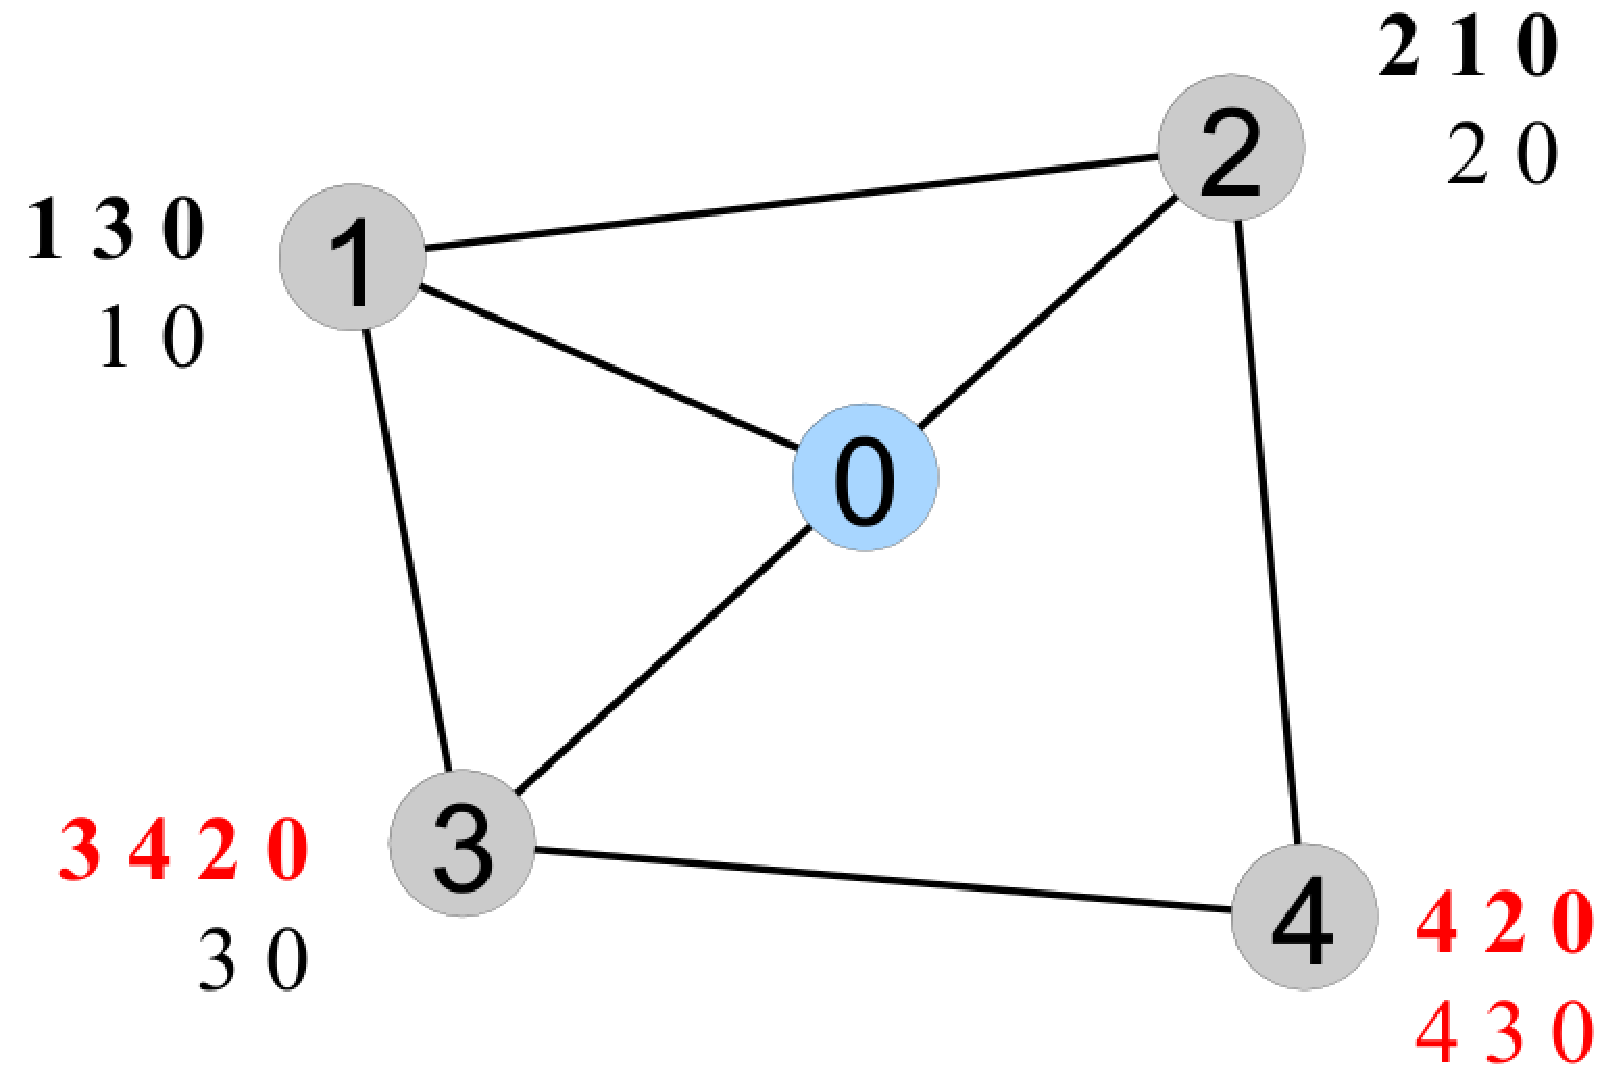
\includegraphics[width=0.5\textwidth]{fab_019.pdf}

\begin{tabular}{|c|c|c|c|c|}
  \hline
  Pas & Noeud 1 & Noeud 2 & Noeud 3 & Noeud 4 \\
  \hline
  0 & (1 0) & (2 0) & (3 0) & \\
  & (1 0) & (2 0) & (3 0) & \\
  \hline
  1 & (1 0), (1 3 0) & (2 0), (2 1 0) & & (4 2 0), (4 3 0) \\
  & (1 3 0) & (2 1 0) & & (4 2 0) \\
  \hline
  2 & & (2 0) & (3 0), (3 4 2 0) & (4 3 0) \\
  & & (2 0) & (3 4 2 0) & (4 3 0) \\
  \hline
  3 & (1 0) & & (3 0) & (4 2 0) \\
  & (1 0) & & (3 0) & (4 2 0) \\
  \hline
  4 & (1 0), (1 3 0) & (2 0), (2 1 0) & (3 0), (3 4 2 0) & (4 2 0), (4 3 0) \\
  & (1 3 0) & (2 1 0) & (3 4 2 0) & (4 2 0) \\
  \hline
  5 & (1 0) & (2 0) & & $\emptyset$ \\
  & (1 0) & (2 0) & & $\epsilon$ \\
  \hline
  6 & & (2 0), (2 1 0) & (3 0) & (4 2 0) \\
  & & (2 1 0) & (3 0) & (4 2 0) \\
  \hline
  7 & (1 0), (1 3 0) & & (3 0), (3 4 2 0) & (4 3 0) \\
  & (1 3 0) & & (3 4 2 0) & (4 3 0) \\
  \hline
  8 & (1 0) & (2 0) & (3 0) & $\emptyset$ \\
  & (1 0) & (2 0) & (3 0) & $\epsilon$ \\
  \hline
  ... & ... & ... & ... & ...
\end{tabular}

Mauvaise nouvelle: la solvabilité est NP-complète, malgré ce résultat,
des choses intéressantes peuvent malgré tout être dites.

Par exemple, ce n'est pas parce qu'un système est solvable qu'il
convergera forcément. Une instance SPP est sûre si elle est solvable
sous n'importe quelle séquence d'activation où aucune information
n'est perdue.

\paragraph{Roues de dispute}

On peut voir DISAGREE comme une roue de dispute à deux rayons.

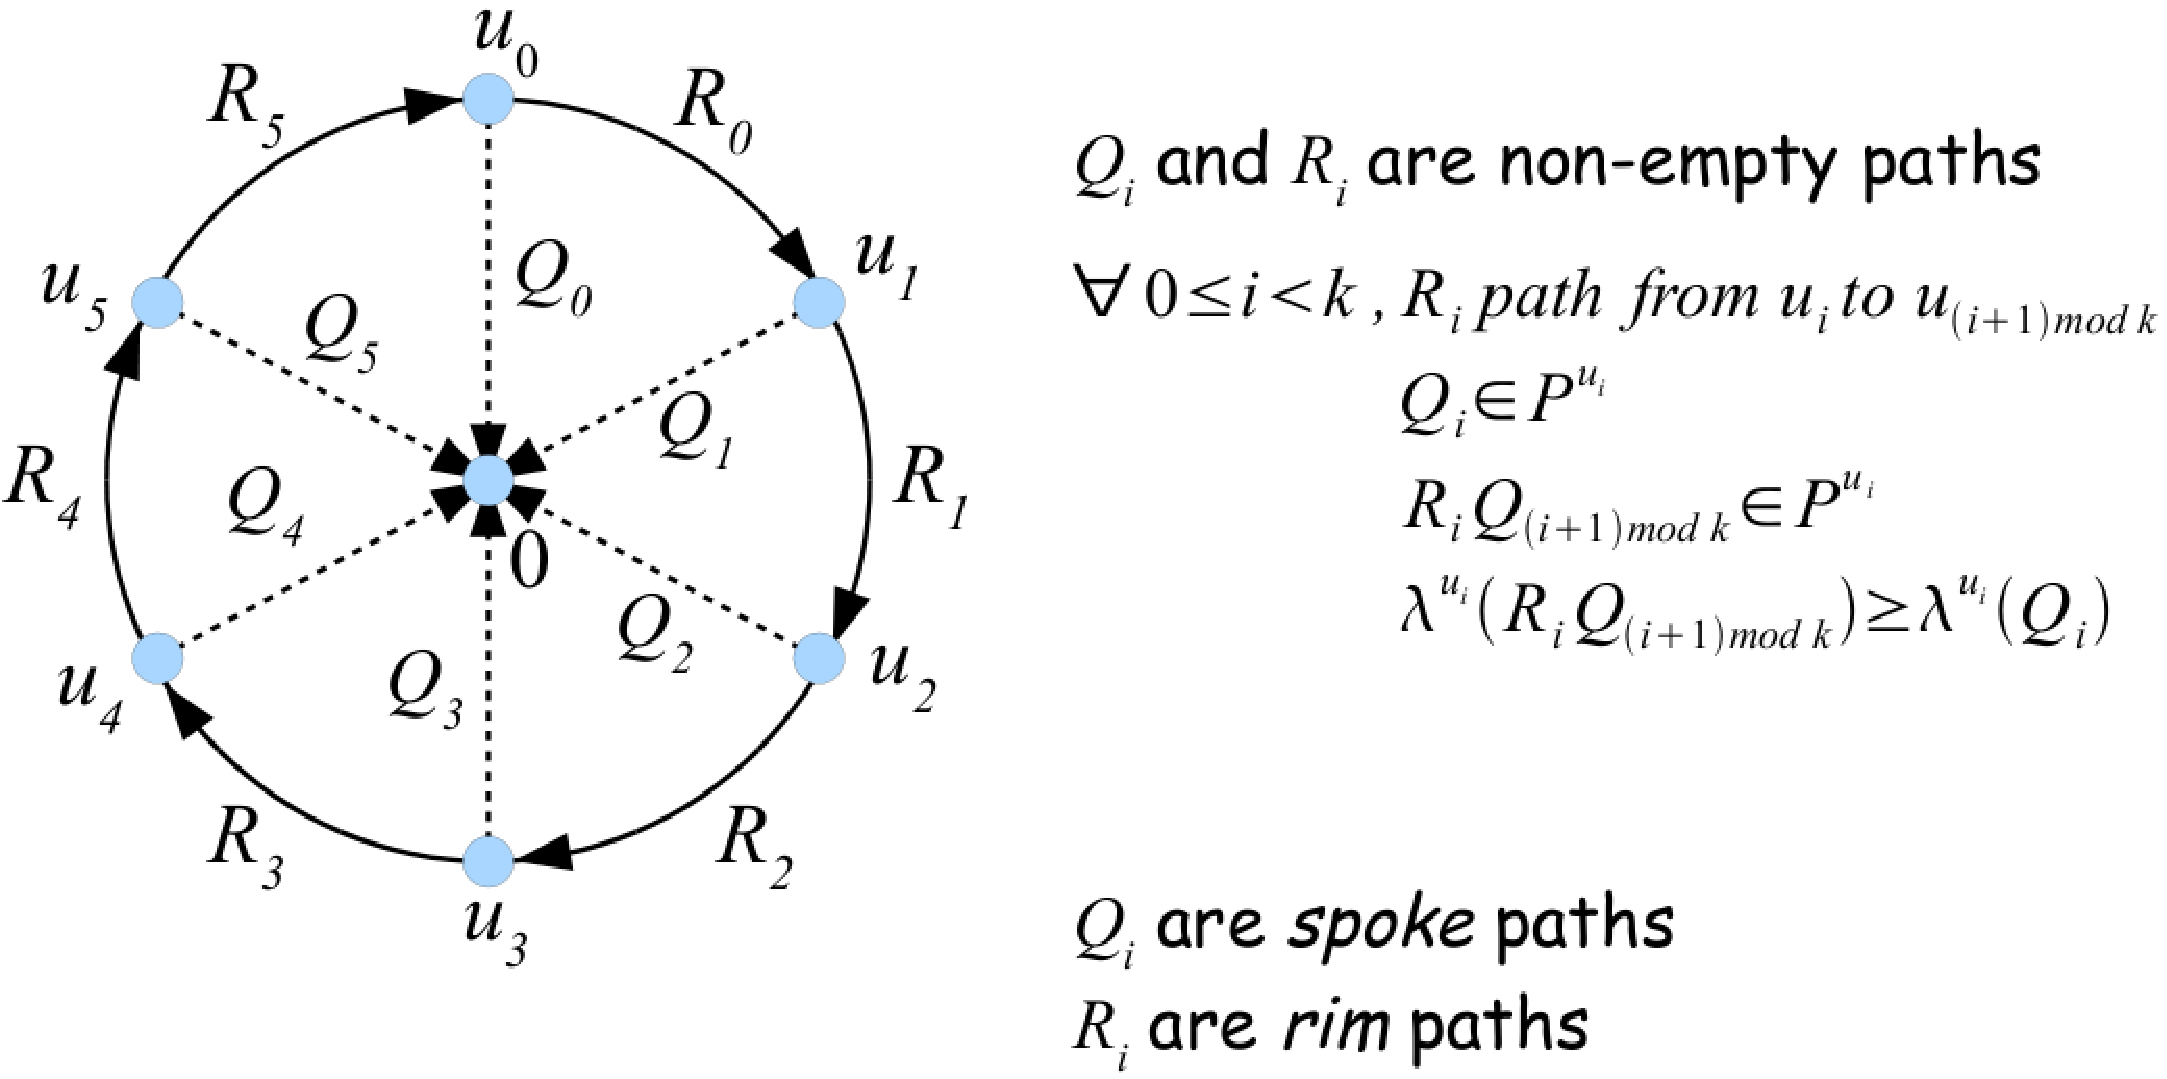
\includegraphics[width=\textwidth]{fab_020.pdf}

Théorèmes: Si une instance SPP n'a pas de roue de dispute, alors elle
est solvable, a une solution unique et est sûre.

\paragraph{Limitations}

Le formalisme SPP est difficile à appliquer directement à un système
BGP car les fonctions de rang ne sont pas explicites dans les filtres
de routage BGP.

Le condition ``Pas de roue de dispute'' est trop forte dans certains
cas.

Les politiques de routage ne sont toujours pas bien comprises et font
l'objet de beaucoup de recherches.

Toutefois, des études ont prouvé que si chaque AS suit les deux lignes
directrices suivantes, alors le système serait sûr:

\begin{itemize}
\item Ranger les routes de telle sorte que celles des clients soient
  préférées à celles des pairs, qui elles-mêmes doivent être préférées
  à celles des fournisseurs.
\item Filtrer les routes pour que les chemins entre fournisseurs et/ou
  pairs ne soient pas autorisés.
\end{itemize}

\subsubsection{Problèmes d'iBGP}

\begin{itemize}
\item Les routes peuvent osciller à cause du MED
\item BAD GADGET peut être ``implémenté'' en iBGP
\item On peut créer des boucles de forwarding en iBGP
\end{itemize}

\section{IPv6}

\subsection{Motivations}

Les motivations principales sont :
\begin{itemize}
\item le manque d'adresses IPv4,
\item le format des paquets IPv4 est complexe,
\item le forwarding IPv4 est difficile à implémenter en hardware,
\item des manques dans IPv4 comme de la configuration automatique, des qualités de services différentes, améliorer la sécurité 
et la mobilité, ... , \\
\end{itemize}

\noindent Pour le moment on résout le manque d'adresses grâce aux \textbf{NAT} \textit{(Network Address Translation)} ce qui 
permet en plus de cacher les adresses privées d'un réseau à l'internet. Cependant, traverser un \textbf{NAT} peut être 
compliqué, c'est également contre le principe de conversation "end-to-end" et ça donne un faux sentiment de sécurité. Il se peut 
également que les noeuds modifient le contenu d'un paquet (changer les adresses, les informations TCP/UDP,...).

\subsection{Architecture d'adressage}

Les adresses sont stockées sur 128 bits, ce qui fait $2^{128}$ adresses différentes soit $3,4 * 10^{38}$. Elles sont de $3$ 
types :
\begin{itemize}
\item les adresses \term{unicast} : adresse identifiant une seule interface. Un paquet envoyé à une telle adresse est délivrée à 
l'interface identifiée par cette adresse. Dans ces adresses on compte : \\
\begin{itemize}
\item $0:0:0:0:0:0:0:0$ ($::$), l'adresse non-spécifiée,
\item $0:0:0:0:0:0:0:1$ ($::1$), l'adresse de loop-back.
\end{itemize}
\item les adresses \term{anycast} : adresse identifiant un pack d'interfaces (en général sur différents équipements). Un paquet 
envoyé à une telle adresse est remis à l'interface identifiée par cette adresse la \textit{plus proche}. Ca fonctionne bien 
pour les transactions sans états (UDP par exemple).
\item les adresses \term{multicast} : adresse identifiant un pack d'interfaces. Un paquet envoyé à une telle adresse est 
délibrée à toutes les interfaces identifiées par cette adresse. Par exemple, tous les pc's, GSM's ou autres doivent appartenir 
au groupe $FF02::1$, tous les routeurs à $FF02::2$,  ... \\
\end{itemize}

De plus, les adresses seront fortement agrégeables, si une entreprise change de provider elle devra réaffecter des nouvelles 
adresses à ses interfaces. Aussi, si un sous-réseau est le "fils" de 2 réseaux différents, il aura une adresse pour chacun de 
ses 2 "pères" (il pourra alors être joint par l'un ou par l'autre avec l'adresse correspondante). \\

Il existe également un mécanisme permettant à 2 matériels proches, connectés sur le même lien ou LAN désireux de communiquer 
sans avoir accès à l'internet global. Chacune de ces adresses, appelées Link-local addresses, commence par FE8 (on peut par 
exemple les construire à partir de l'adresse MAC).

\subsection{Paquets IPv6}

\begin{figure}[h!]
    \begin{center}
    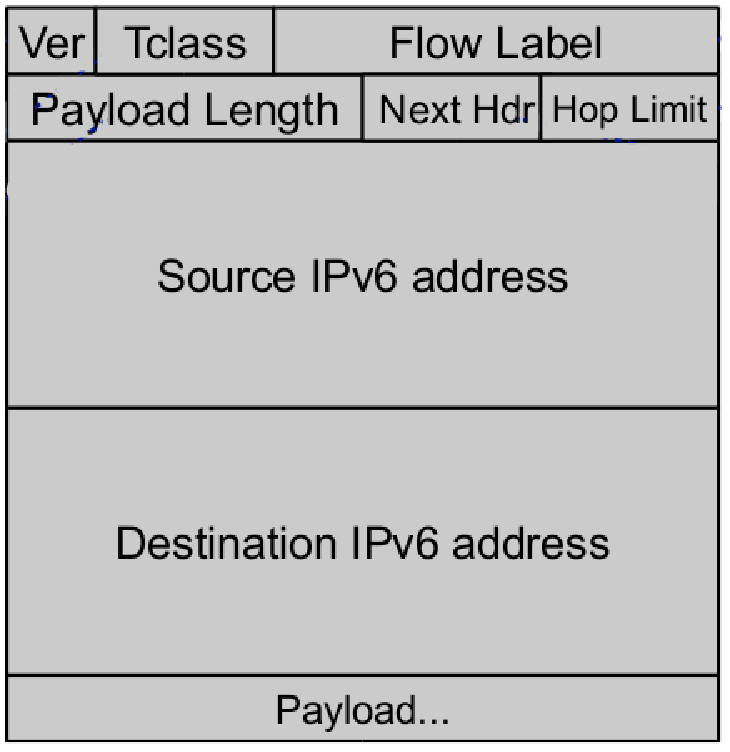
\includegraphics[width=200px]{img_003.pdf}
    \caption{Représentation d'un paquet IPv6}
    \end{center}	
\end{figure}

\begin{itemize}
\item Tous les champs sont alignés en blocs de 32 bits pour faciliter l'implémentation.
\item Le TTL qui se renomme en Hop Limit.
\item Next Hdr représente le type du payload (ex si $=6$, le payload est un paquet TCP, il faut donc lire un header TCP, les 
headers étant chaînés les uns à la suite des autres). \\
\end{itemize}

IPv6 réclame un MTU minimum de 1280 bytes et la fragmentation n'est plus possible. Si elle est tout de même nécessaire, il faut 
fragmenter au niveau du cable, IPv6 ne s'en occupe pas (seuls les noeuds en fin de parcours ou en début de parcours font de la
fragmentation/reconstitution avec le header d'extension de fragment).

\begin{figure}[h!]
    \begin{center}
    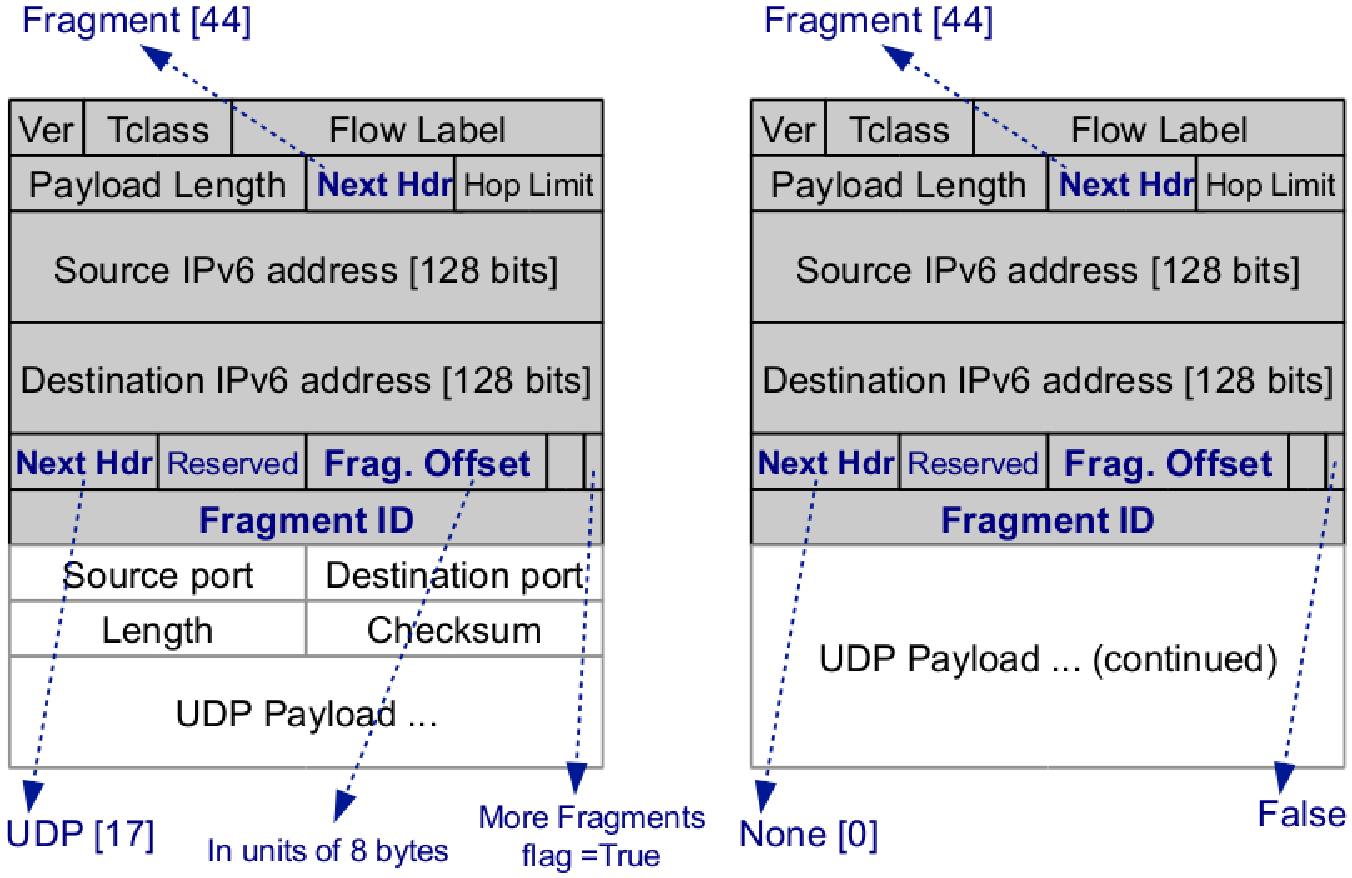
\includegraphics[width=250px]{img_004.pdf}
    \caption{Exemple de fragmentation en IPv6}
    \end{center}	
\end{figure}

\subsection{ICMPv6}

Il remplace l'\textbf{ARP} d'IPv4 en ce qui concerne la découverte de voisins. Il permet d'envoyer un message de sollicitation 
de voisin à l'adresse broadcast des noeuds sollicités ($FF02::1:FFxx:xxxx$) et de répondre par un message d'avertissement aux 
voisins qui ont envoyé une sollicitation (ou en multicast si la source n'était pas spécifiée).\\

Grâce aux messages ICMPv6 \textit{(Internet Control Message Protocol)}, IPv6 est capable d'\term{auto-configuration} 
(\textbf{SLAAC}, \textit{StateLess Address Auto-Configuration}). Cette auto-configuration utilise la découverte de voisins, la 
détection d'adresse dupliquée (DAD), la découverte de routeur ainsi que des préfixes et des paramètres des liens. Pour obtenir 
une adresse IPv6, un matériel peut avoir recours à différentes techniques. Soit comme en IPv4, manuellement codée par un 
opérateur ou via un serveur DHCPv6, soit via l'\term{auto-configuration} spécifiée ci-dessus. Celle-ci fonctionne comme suit :
\begin{figure}[h!]
    \begin{center}
    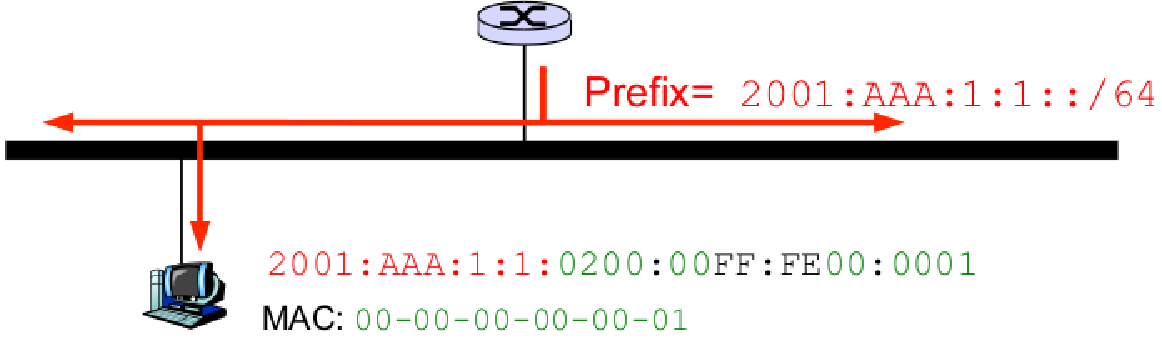
\includegraphics[width=225px]{img_005.pdf}
    \caption{Auto-configuration}
    \end{center}	
\end{figure}
\begin{itemize}
\item Le routeur envoie un préfixe en multicast ($FF02::1$),
\item Les hôtes convertissent leur adresse MAC en format 64 bits (EUI-64) et la concatène au préfixe reçu du routeur
\end{itemize}

Lorsqu'un ordinateur démarre, il utilise son adresse link-local pour envoyer des messages ICMPv6 en vue de l'obtention d'une 
adresse IPv6. Il se peut cependant qu'un autre matériel possède la même adresse link-local (typiquement 2 matériels ayant la 
même adresse MAC ou des adresses configurées manuellement). Il doit donc détecter si quelqu'un utilise cette adresse, il 
utilise le DAD.

\begin{figure}[h!]
    \begin{center}
    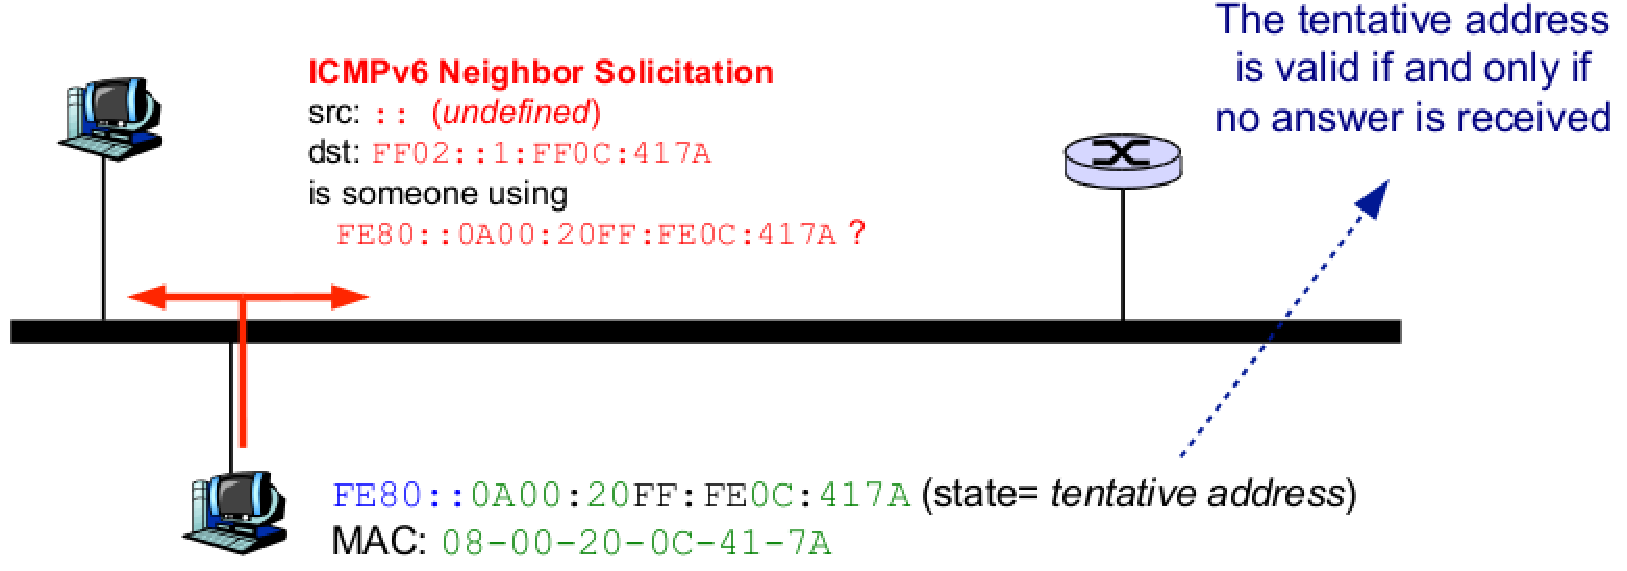
\includegraphics[width=200px]{img_006.pdf}
    \caption{Dupplicate Address Detection}
    \end{center}	
\end{figure}

Il envoie un message de sollicitation à l'adresse multicast des noeuds sollicités correspondant à l'adresse qu'il désire 
employer. (Le noeud doit souscrire à l'adresse multicast de tous les noeuds $(FF02::1)$ et à l'adresse multicast de tous les 
noeuds sollicités $(FF02::1:FFxx:xxxx)$ de l'adresse désirée. Une fois qu'il a son adresse link-local, il peut soit attendre 
que le routeur envoie son préfixe soit il peut lui envoyer un \textit{router solicitation} afin que celui-ci lui envoie son 
préfixe. (Il faudra utiliser le DAD pour la nouvelle adresse créée également) \\

Le problème dans tout ça c'est que ces adresses auto-configurées utilisent les adresses MAC des composants, adresses qui sont 
fixes et uniques. Ainsi, n'importe qui peut être traqué très facilement $\Rightarrow$ problème de confidentialité ! On préfèrera 
donc l'emploi d'un serveur DHCPv6 configuré pour ne jamais réallouer la même adresse. On peut également autoriser les hôtes à
utiliser des identifications d'hôtes aléatoires dans les 64 bits de poids les plus faibles de leur adresse IPv6. \\

Se pose maintenant le problème de la sécurité. En effet, il se peut qu'un utilisateur décide d'annoncer un faux neighbour 
solicitation ou un faux neighbour advertisement. Pour pallier à ça, la solution est le \term{CGA} \textit{(Cryptographically 
Generated Addresses}. Chaque noeud possède sa clé privée et sa clé publique, chacun de ses noeuds aura pour adresse IPv6 le 
préfix du réseau + l'identifiant du subnet + la clé publique. Chaque noeud enverra donc ses données encryptées grâce à sa clé 
privée et le noeud la recevant utilisera la clé publique pour décrypter le message. Le problème c'est que les adresses IPv6 sont 
de taille fixe, et la partie disponible pour la clé publique est de 62 bits. Or une clé publique RSA de 62 bits ce n'est pas 
sécuritaire (au moins 1024 bits sont recommandés). L'idée est de prendre comme identifiant une fonction de hashage calculée sur 
la clé publique (en ignorants les 2 bits spéciaux pour la transformation en EUI-64). Ainsi, de manière simplifiée on a :
\begin{enumerate}
\item L'hôte A choisit une paire de clés ($Pub_A$, $Priv_A$), et définit son identifiant d'hôte $HostId_A$ comme $Hash_{64}
(Pub_A)$.
\item Un hôte B envoit une sollicitation de voisin pour l'adresse $prefix:HostId_A$ (prefix étant le préfixe du router).
\item A répond par un Neighbour Advertisement ($NA$) signé avec $s = E(H(NA),Priv_A)$ (E = encrypt). Il fournit également sa 
clé publique et son adresse de la couche lien.
\item B vérifie que $Hash_{64}(Pub_A) = HostID_A$ et que $D(s,Pub_A) = H(NA)$ (D = decrypt).
\end{enumerate}

Le problème de \textbf{CGA} est qu'un hashage de 62 bits n'est pas vraiment sécurisant, en effet une attaque brute-force avec un
dictionnaire peut avoir raison assez vite de ce système. L'idée pour résoudre ce problème est alors de calculer une plus grande
valeur de hashage et d'en donner qu'une partie (la partie restante étant connue) et c'est ce qui est utilisé en pratique.

\subsection{DNSv6}

\noindent Chaque message DNS est composé de \term{Resource Record}'s (\textbf{RR}) encodés sous forme d'un quadruplet\\
$(Name,Value,Type,TTL)$. Ces \term{RR} sont de plusieurs types :
\begin{itemize}
\item \blu{$A$}, $Name$ représente alors un nom de domaine et $Value$ une adresse \textbf{IPv4},
\item \blu{$AAAA$}, $Name$ représente alors un nom de domaine et $Value$ une adresse \textbf{IPv6},
\item \blu{$NS$}, $Name$ représente alors un nom de domaine et $Value$ est le nom d'hôte d'un serveur \textbf{DNS} responsable 
pour $Name$,
\item \blu{$MX$}, identique pour les mails,
\item \blu{$CNAME$}, pour les alias.\\
\end{itemize}

Les DNS ont du être adaptés un tant soit peu pour supporter IPv6, ils ont par exemple été modifié pour supporter des réponses 
plus longues.

\subsection{Transition d'IPv4 à IPv6}

Il n'y aura pas de jour limite où tout le monde devra passer à IPv6, il faut donc qu'internet supporte les 2 versions. Pour celà 
il y a plusieurs mécanismes :
\begin{itemize}
\item \titre{La dual-stack}, les noeuds suivant ce mécanisme possèdent un support pour les 2 protocoles. Ils agissent comme 
routeur IPv6/IPv4 lorsqu'ils communiquent avec d'autres noeuds IPv6/IPv4. Ceci impliquant un besoin de stockage plus grand car 
il faut tout stocker en double, comme une table de forwarding pour chacun par exemple.
\item \titre{Le tunneling}.
\item \titre{La traduction} qui consiste à employer des adresses IPv6 particulières dont la partie d'identification de l'hôte 
est une adresse IPv4. Un paquet IPv6 est alors transformer en paquet IPv4 par un NAT. Les soucis sont, entre autres, qu'il y a 
des champs du header IPv6 qui ne sont pas transformables en champs IPv4 et inversément, la fragmentation n'est pas supportée 
par IPv6, cela prend du temps et de la mémoire, il y a des contraintes sur la topologie (toutes les réponses doivent venir par 
le même NAT).
\end{itemize}

\section{MPLS}

La principale motivation de \term{MPLS} \textit{(MultiProtocol Label Switching)} est de supporter de manière efficace des 
réseaux à grande vitesse c'est-à-dire rendre capable les routeurs de travailler sur un paquet et de le forwarder sur la bonne 
interface à la vitesse de la ligne. Il permet également d'effectuer du \term{Traffic Engineering}, il est utile pour les VPN's 
\textit{(Virtual Private Network)} et est aussi très rapide au niveau de la restauration. Ce protocole utilise la technique du 
\term{Label Swapping}. Cette technique consiste à ce qu'un routeur analyse le label contenu par un paquet qu'il a reçu et 
l'interface d'où il est venu. Sur base de ces 2 informations (via une table de forwarding par label ($LFIB$)), le routeur 
décide sur quelle interface il doit pousser le paquet et quel label il doit lui accrocher.

\begin{figure}[h!]
    \begin{center}
    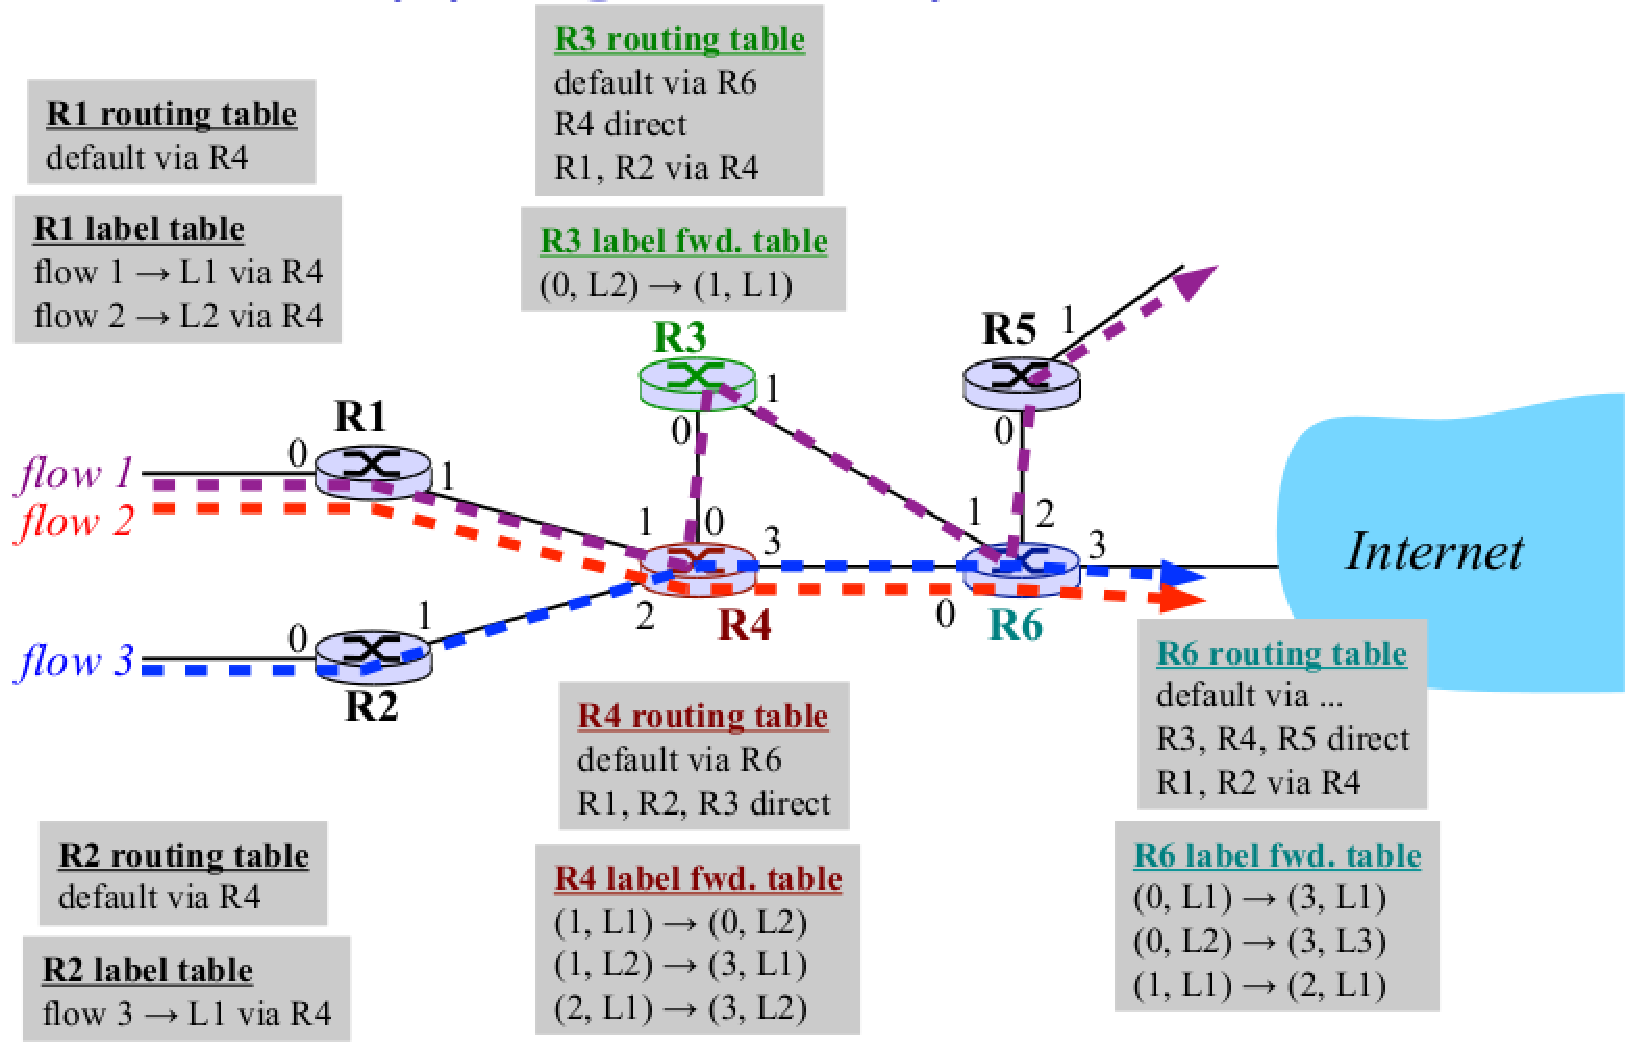
\includegraphics[width=300px]{img_007.pdf}
    \caption{Exemple de Label Swapping}
    \end{center}	
\end{figure}

\subsection{Utiliser le label swapping et IP}

L'objectif ici est d'utiliser le label swapping à l'intérieur d'un réseau et d'utiliser IP en dehors de celui-ci pour joindre 
d'autres réseaux. Pour construire un paquet IP contenant un label, il convient d'introduire un header spécifique de $32$ bits en 
début de datagramme IP. Dans ce header, 20 bits sont réservés au label, ce qui offre $2^{20} = 1048576$ possibilités de labels 
différents. Un routeur pour alors effectuer 3 opérations :
\begin{enumerate}
\item \blu{\textbf{PUSH}}, qui consiste à ajouter un label en début du datagramme IP,
\item \blu{\textbf{SWAP}}, qui consiste à modifier le label en début du datagramme IP,
\item \blu{\textbf{POP}}, qui consiste à enlever le label en début du datagramme IP.
\end{enumerate}
Une \term{LFIB} est donc de la forme :
\begin{tabular}{cccc}
in-port & in-label & next-hop/out-port & opération \\
0 & L1 & 2 & POP
\end{tabular} \\

Un \term{LSR} \textit{(Label-Switching Router)} peut gérer ses 2 labels de 2 façons différentes : soit par interface (et donc 
$2^{20}$ labels par interface) soit par LSR et donc $2^{20}$ labels en tout. Le chemin suivi par un paquet allant d'un ingress 
LSR (routeur d'entrée dans le réseau MPLS) et passant par quelques noeuds du réseau pour arriver à un egress LSR (routeur de 
sortie) est appelé \term{Label Switched Path} (\textbf{LSP}). 

\begin{figure}[h!]
    \begin{center}
    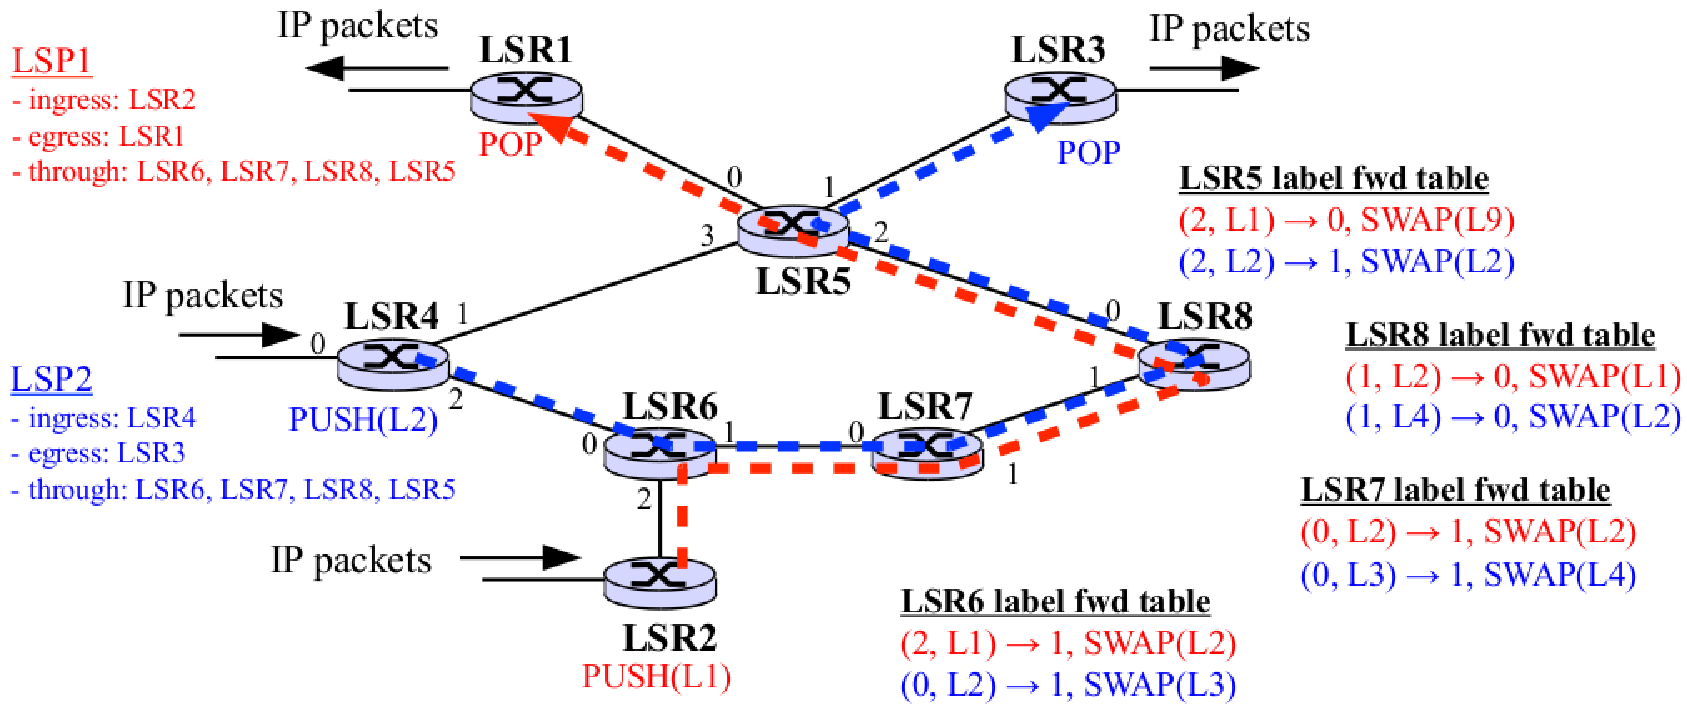
\includegraphics[width=300px]{img_008.pdf}
    \caption{Exemples de LSP}
    \label{lsp1}
    \end{center}	
\end{figure}

Comme on le voit sur la figure \ref{lsp1}, les deux LSP's emprennent le même chemin de LSR6 à LSR5. Il est donc idiot 
d'implémenter 2 passages différents, on crée donc un petit LSP de LSR6 à LSR5 et les 2 autres LSP prendront ce petit LSP pour 
circuler dans le réseau. \\

Comme on le voit, on a besoin de hiérarchiser les LSP. Le bit "stack" du header permet de spécifier que le label courant est au 
sommet de la pile ou pas.
\begin{figure}[h!]
    \begin{center}
    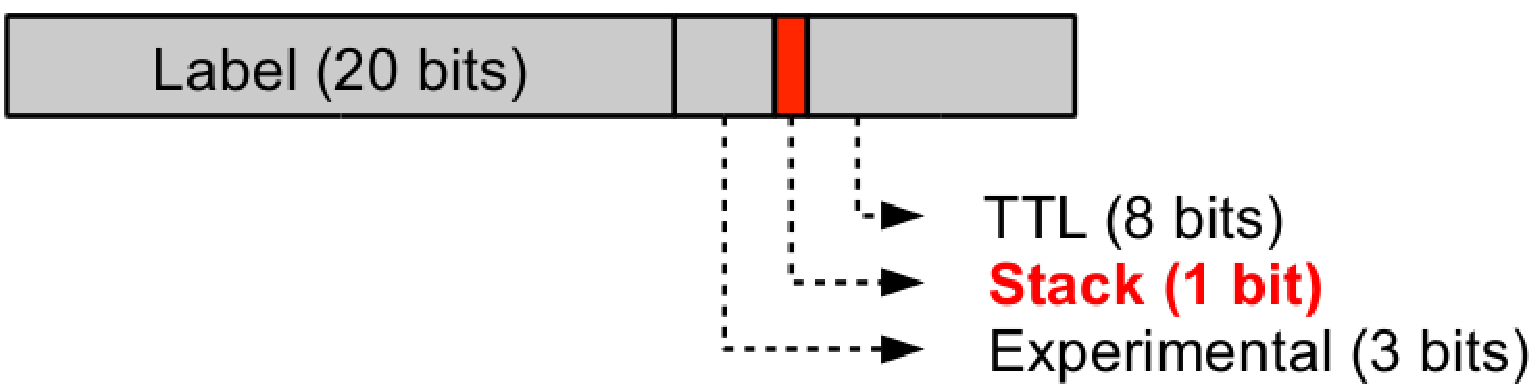
\includegraphics[width=200px]{img_009.pdf}
    \caption{Header MPLS}
    \end{center}	
\end{figure}

\begin{figure}[h!]
    \begin{center}
    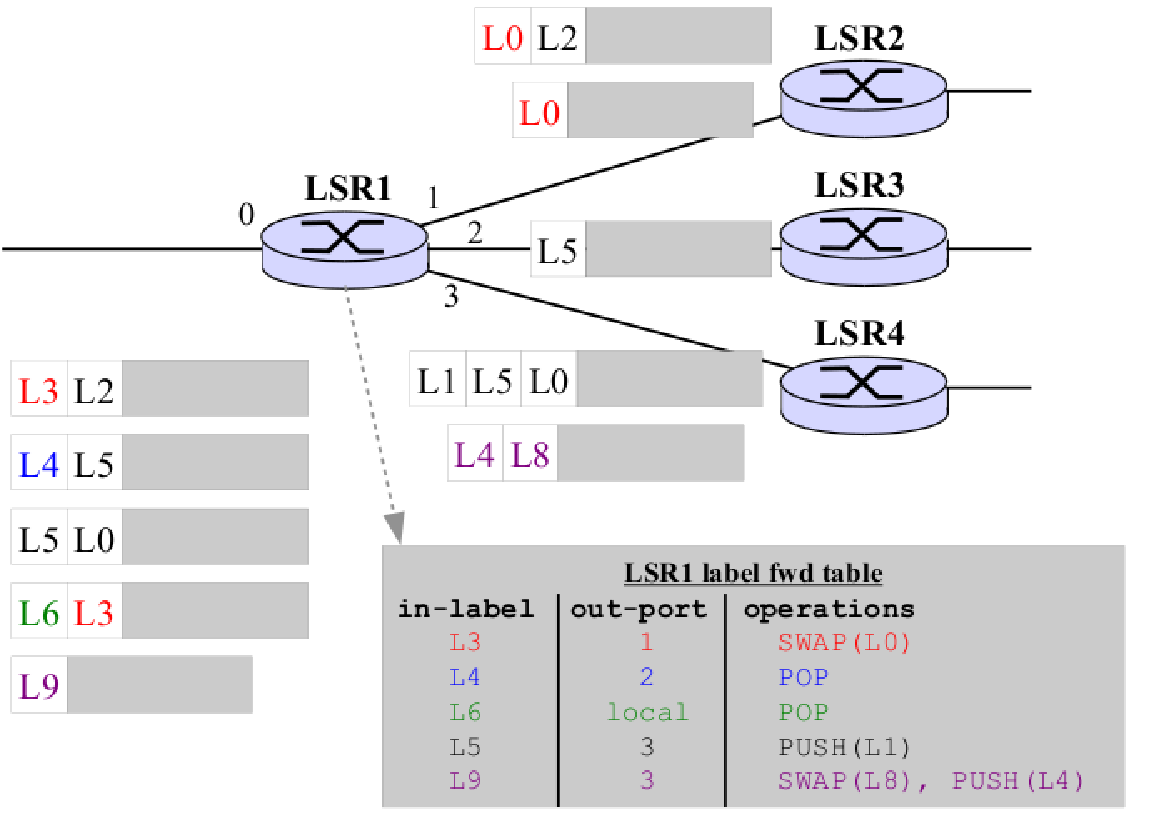
\includegraphics[width=200px]{img_010.pdf}
    \caption{LFIB}
    \end{center}	
\end{figure}

\begin{figure}[h!]
    \begin{center}
    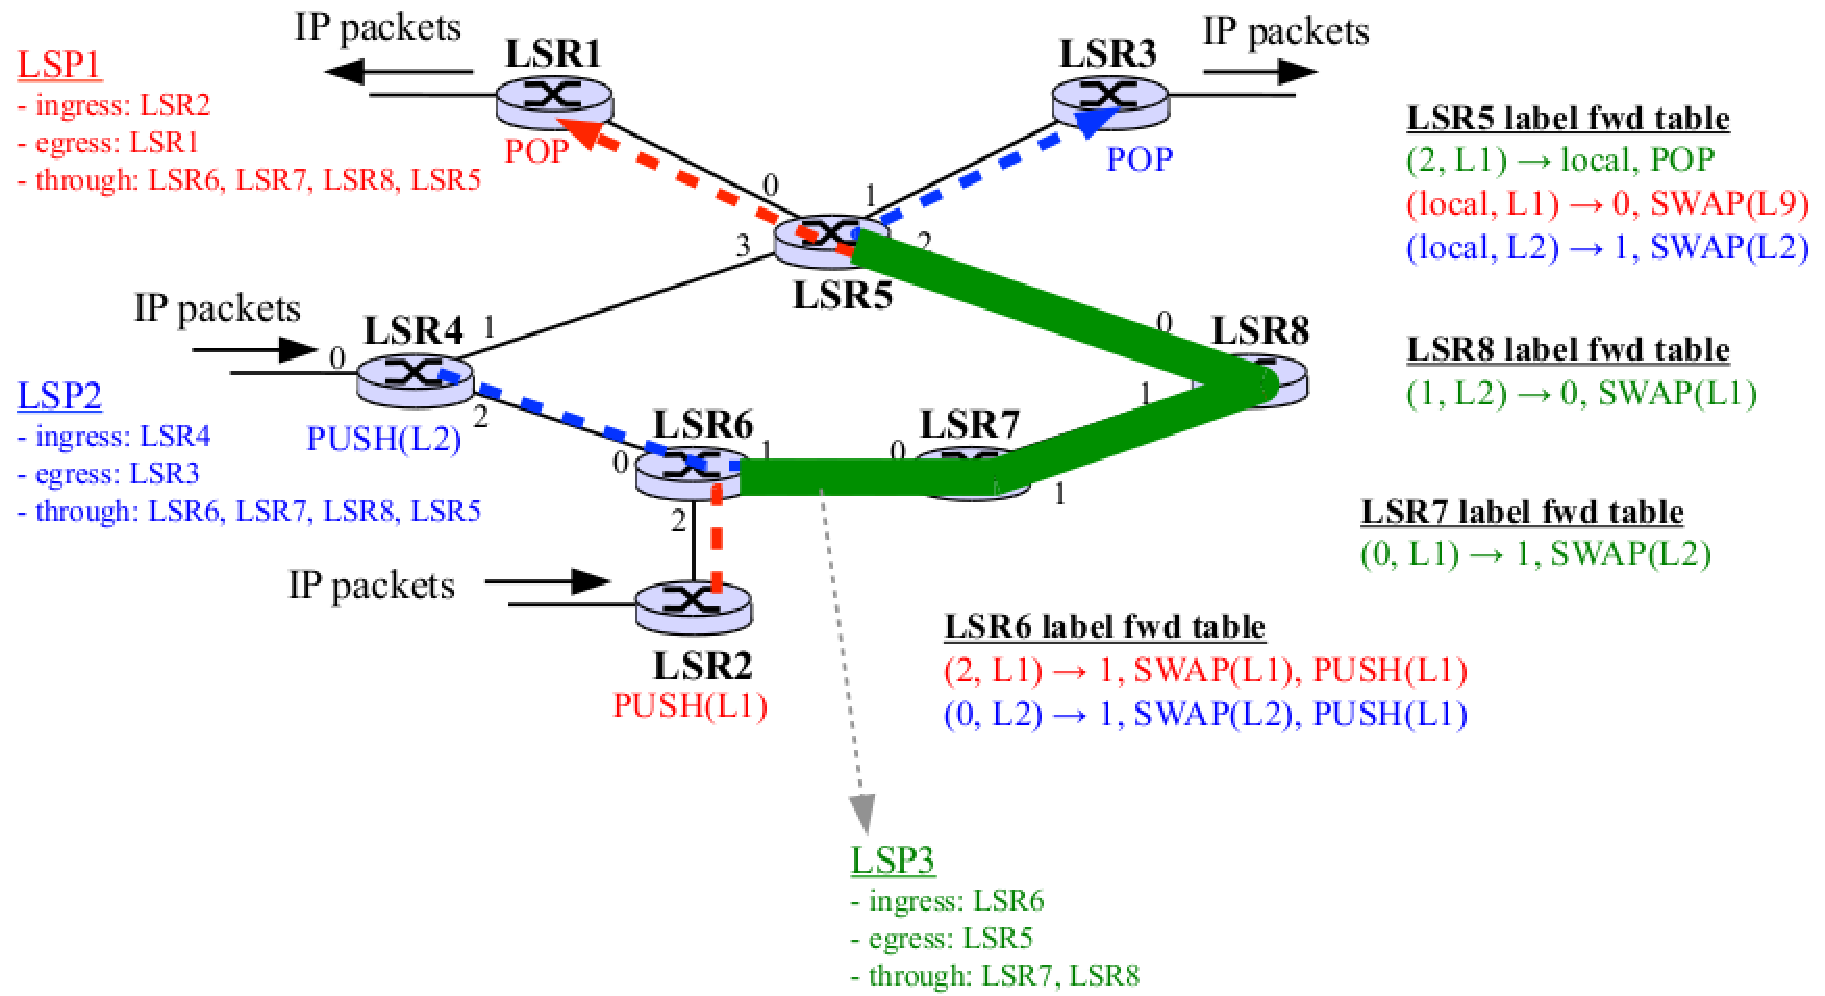
\includegraphics[width=250px]{img_011.pdf}
    \caption{Exemple avec stack}
    \end{center}	
\end{figure}

Les ingress LSR choisissent comment forwarder les paquets IP qu'ils recoivent. Ils définissent des \textbf{FEC} 
\textit{(forwarding equivalence classes)} qui regroupent des paquets IP forwardés de la même façon. 2 paquets d'une même 
\textbf{FEC} auront donc le même label en sortant du ingress LSR. (On peut par exemple définir les \textbf{FEC} par destination, 
tous les paquets ayant même destination seront dans la même \textbf{FEC})

\subsection{Utilisations de MPLS}

\subsubsection*{Forwarding de paquets basé sur la destination}

La question est de savoir comment fournir un service de transit quand les LSR's de bordure sont capables d'attacher et enlever 
des labels, tous les LSR's supportent IP mais que les LSR's internes ne peuvent pas traiter les paquets IP de manière efficace ? 
L'idée est de créer un full mesh de LSP entre chaque paire de LSR de bordure. Il faut trouver dès lors un moyen de le faire
automatiquement et d'enlever certains LSP inutiles. \\

On va utiliser un protocole spécial pour remplir les LFIB de tous les LSR d'un réseau, soit \textbf{LDP} \textit{(Label 
Distribution Protocol} soit \textbf{RSVP-TE}. On pourrait également transporter des mappings FEC-label dans les messages de 
routage échangés par les routeurs mais cela implique que le protocole de routage doit être extensible (c'est le cas de 
\textbf{BGP} mais pas de \textbf{RIP}, \textbf{OSPF} ou encore \textbf{IS-IS} par exemple).

\begin{figure}[h!]
    \begin{center}
    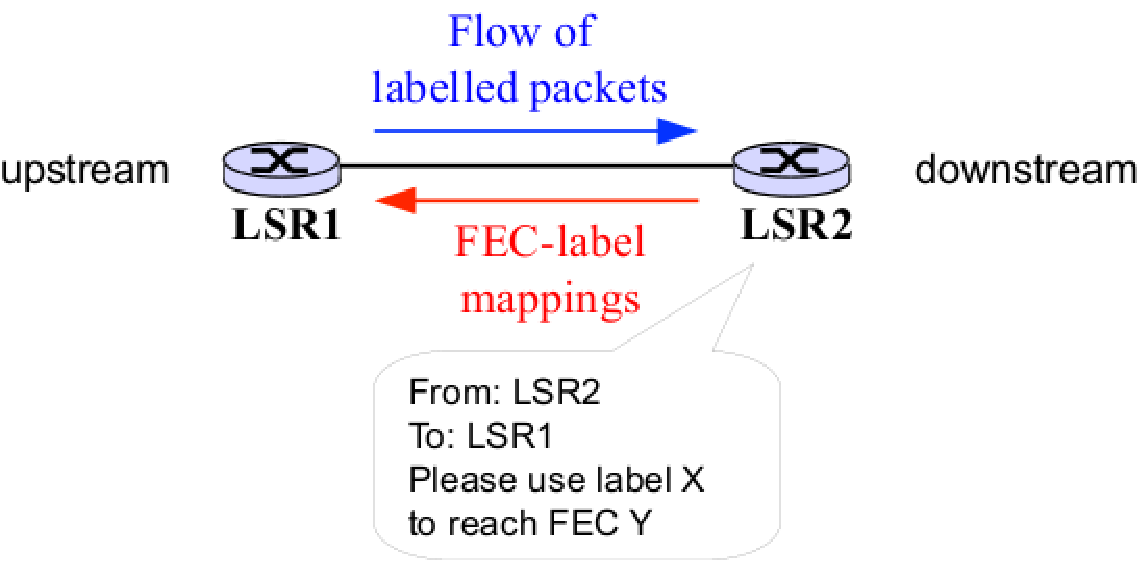
\includegraphics[width=200px]{img_012.pdf}
    \caption{Propagation des messages/mappings}
    \end{center}	
\end{figure}

Ces mappings sont envoyés de 2 façons différentes, soit \blu{sur demande} soit de manière \blu{non-sollicitée}.
\begin{itemize}
\item Dans le premier cas, le LSR en début du flux envoie une requête de label et le LSR en fin de flux répond par un mapping 
FEC-label. \gre{Les avantages de cette méthode sont que les mappings ne sont envoyés que quand c'est nécessaire et les LSR ne 
doivent stocker uniquement que les mappings qui sont utilisés.} \rouge{Les inconvénients sont que lorsqu'un next-hop tombe en 
panne, du temps peut s'écouler avant qu'un label soit demandé au nouveau next-hop.}
\item Dans le second cas, ce sont les LSR en fin de flux qui envoient indépendamment leurs mappings au LSR de début de flux. 
\gre{Les avantages sont que chaque LSR peut recevoir plusieurs labels pour chaque FEC et dans le cas d'une panne passer d'un 
label à l'autre.} \rouge{Les inconvénients sont que les labels ne seront pas distribués au meilleur moment.} \\
\end{itemize}

\subsubsection{LDP}

\term{LDP} utilise \textbf{UDP} pour faire de la découverte de voisins et \textbf{TCP} pour distribuer les mappings selon 
différents modes de transmission qu'il supporte. Il utilise plusieurs types de messages :
\begin{itemize}
\item Initialisation $\rightarrow$ établissement d'une session \textbf{LDP},
\item Keepalive $\rightarrow$ utilisé pour tester que la session est toujours établie,
\item Label mapping $\rightarrow$ utilisé pour annoncer un mapping,
\item Label withdrawal $\rightarrow$ utilisé pour enlever un mapping.
\end{itemize}

Périodiquement les LSR envoient à leurs voisins des messages LDP Hello à l'adresse multicast "tous les noeuds" ($224.0.0.2$), 
ces voisins répondent par un LDP Hello également s'ils sont LSR. LDP possède des qualités telles que la découverte automatique 
des voisins LDP, du transport de confiance, de l'extensibilité et le fait qu'il emploie les chemins les plus courts (ils se 
basent sur les coûts IGP). Voici un exemple d'établissement des liens LDP :

    \begin{center}
    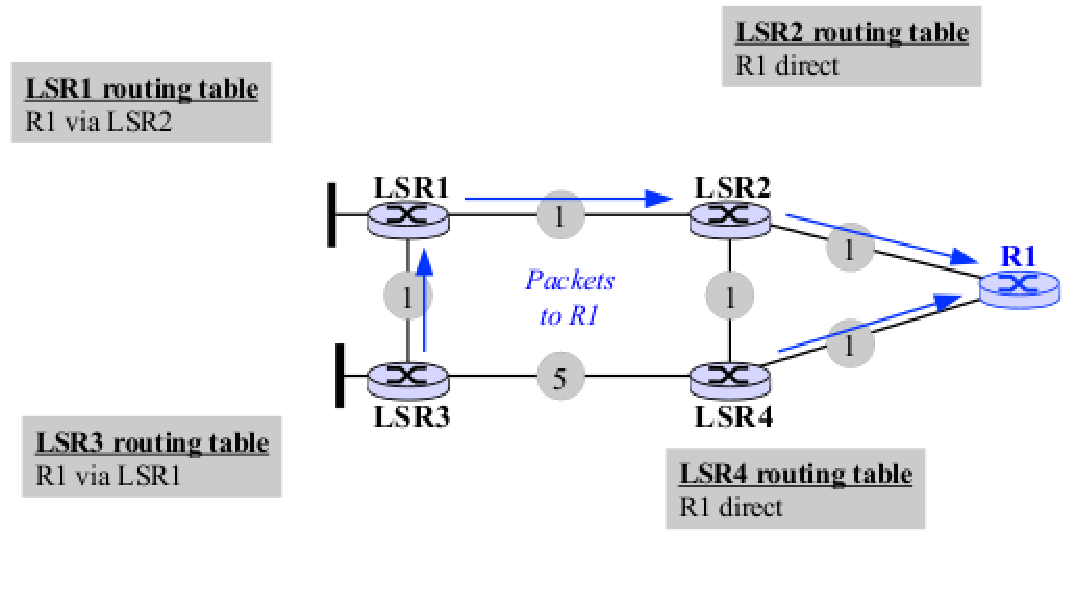
\includegraphics[width=200px]{img_013.pdf}
    \end{center}	

    \begin{center}
    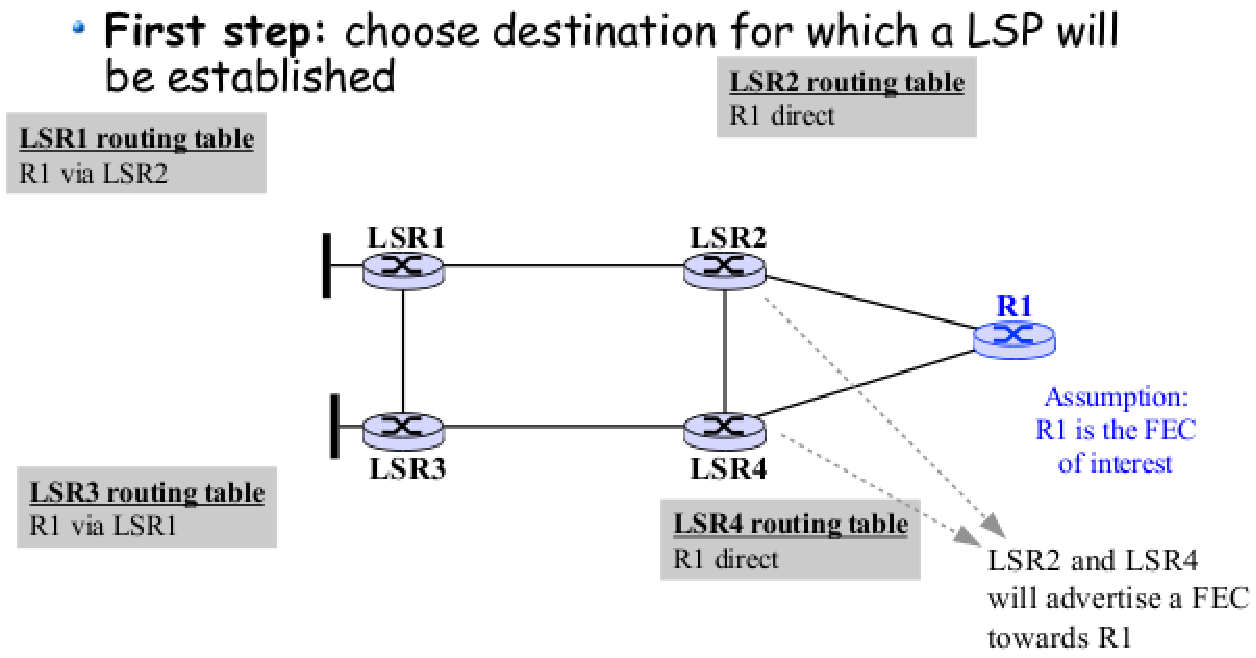
\includegraphics[width=200px]{img_014.pdf}
    \end{center}	

    \begin{center}
    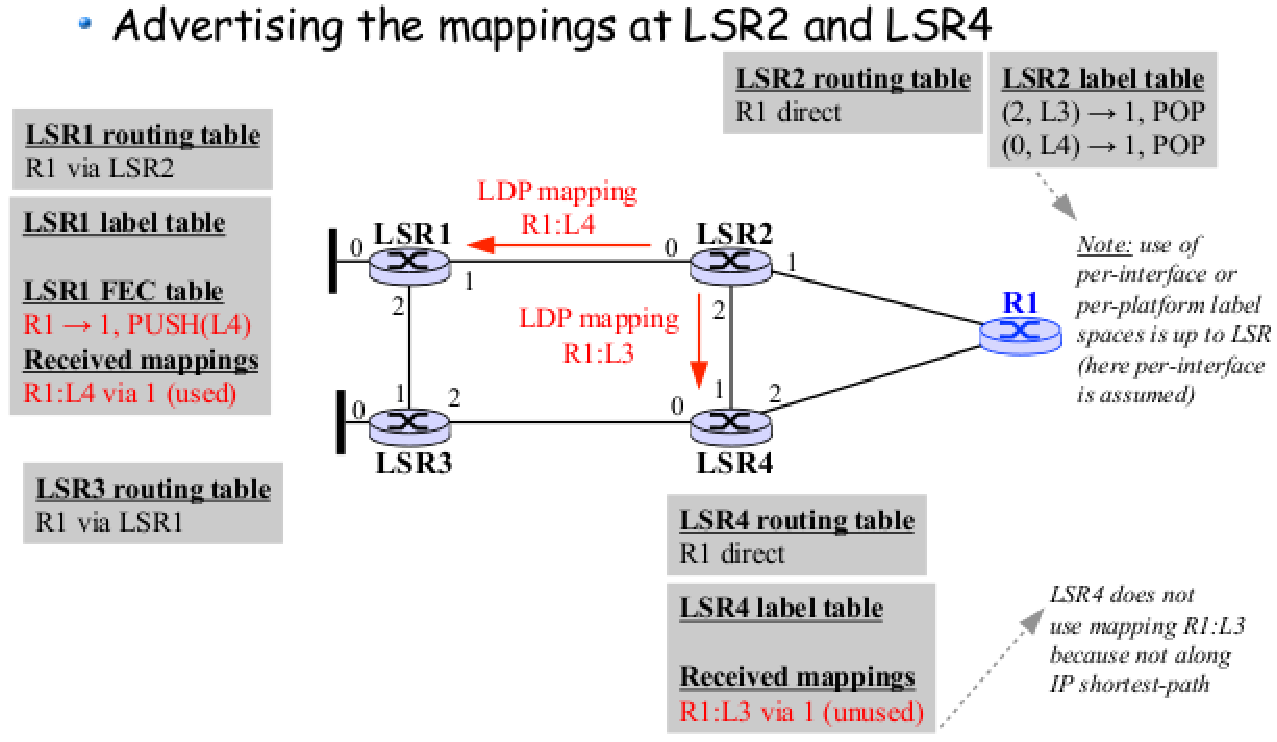
\includegraphics[width=200px]{img_015.pdf}
    \end{center}	

    \begin{center}
    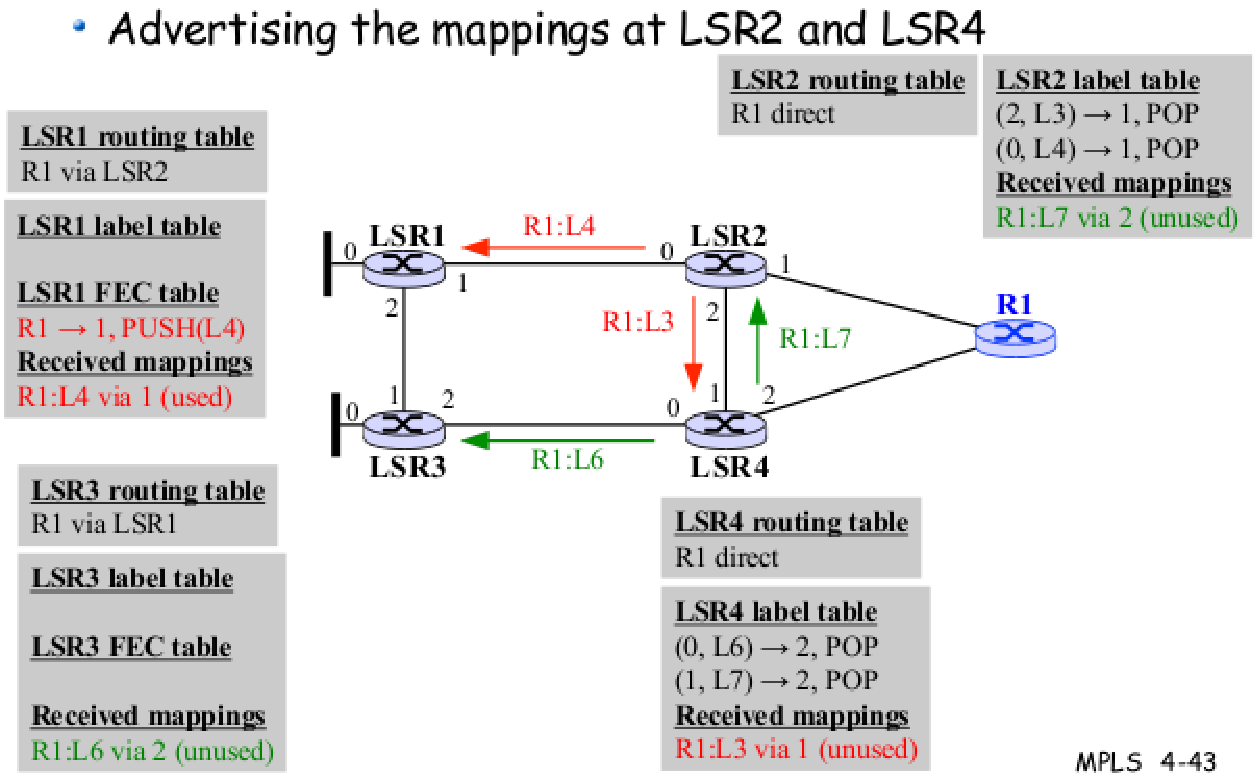
\includegraphics[width=200px]{img_016.pdf}
    \end{center}	

    \begin{center}
    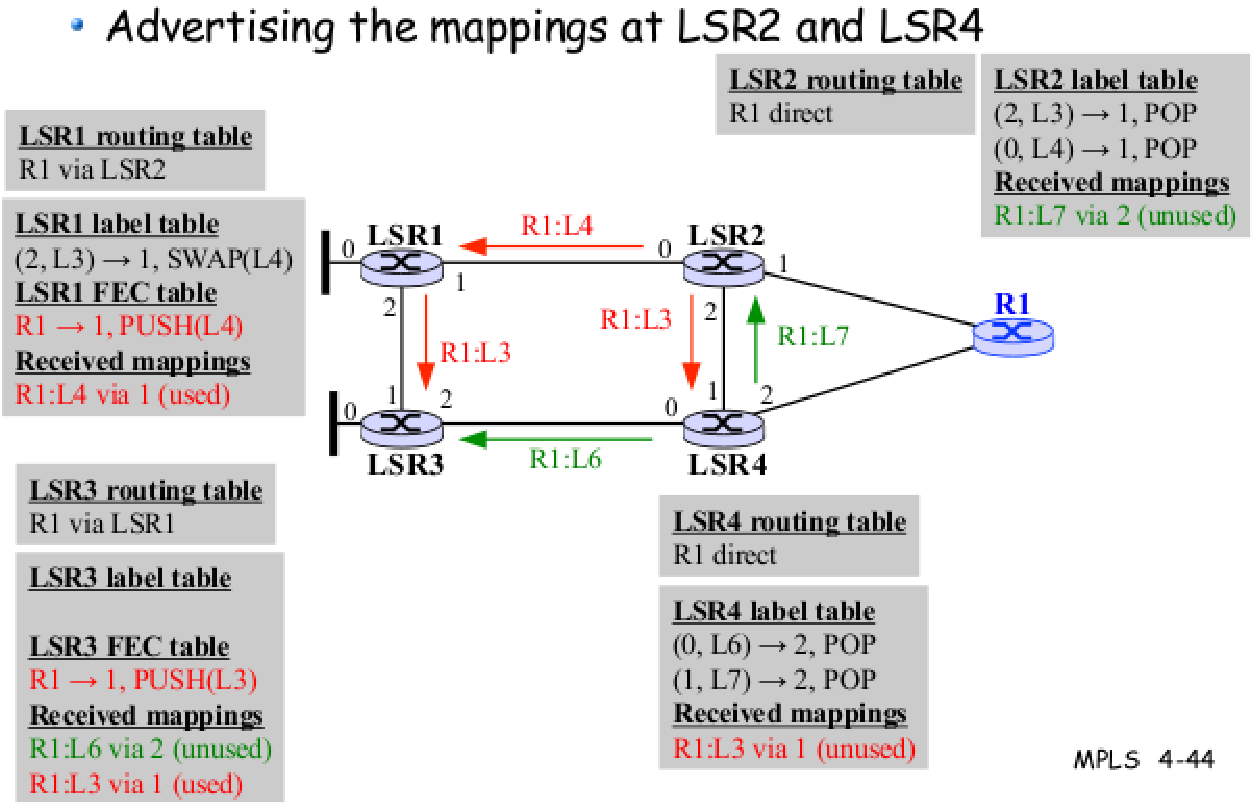
\includegraphics[width=200px]{img_017.pdf}
    \end{center}	

    \begin{center}
    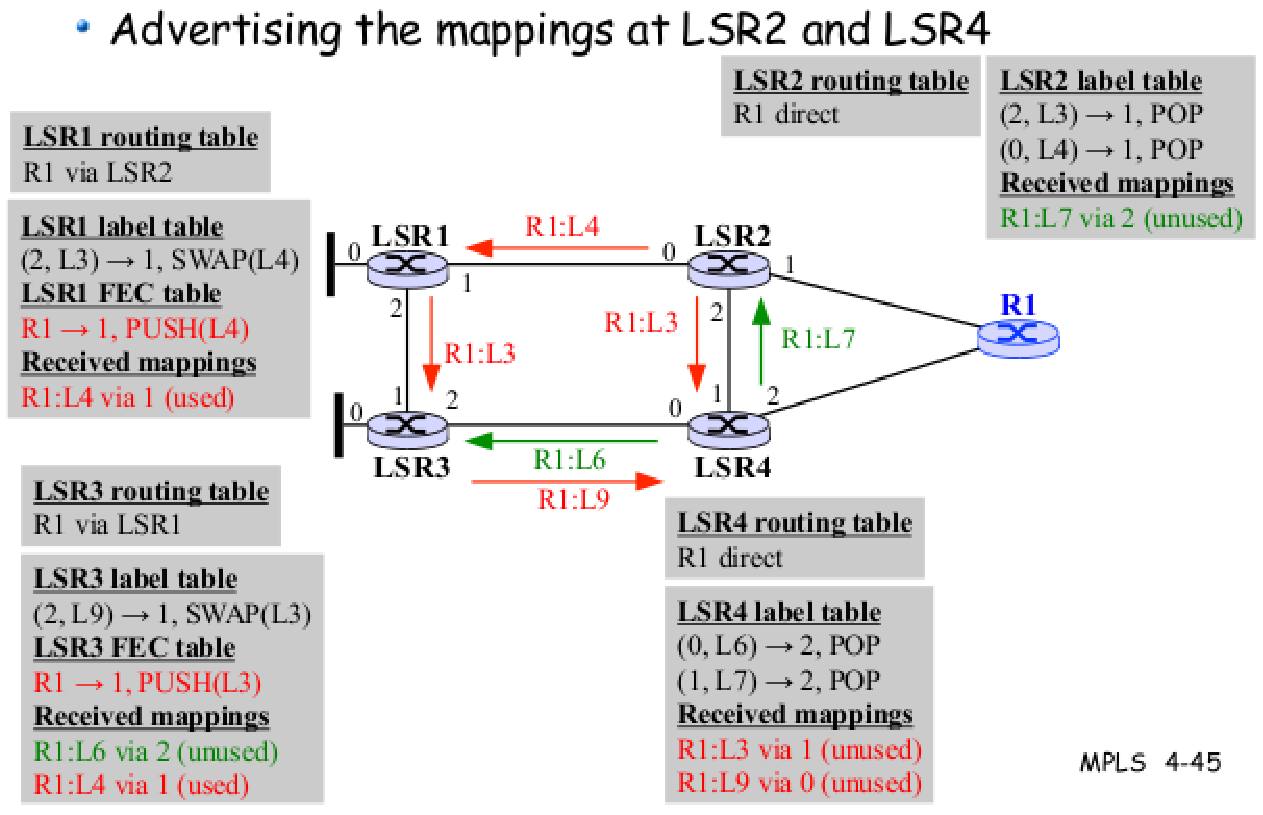
\includegraphics[width=200px]{img_018.pdf}
    \end{center}	

    \begin{center}
    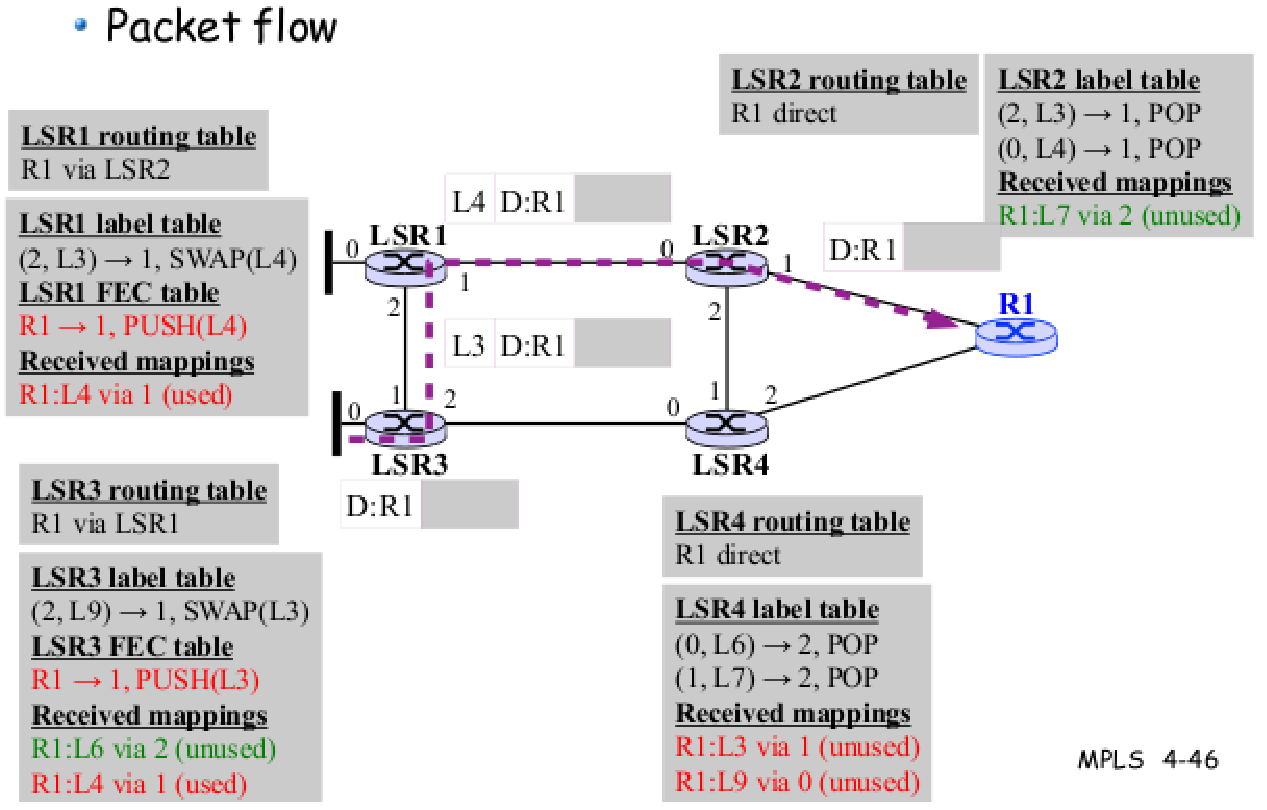
\includegraphics[width=200px]{img_019.pdf}
    \end{center}	

\begin{center}
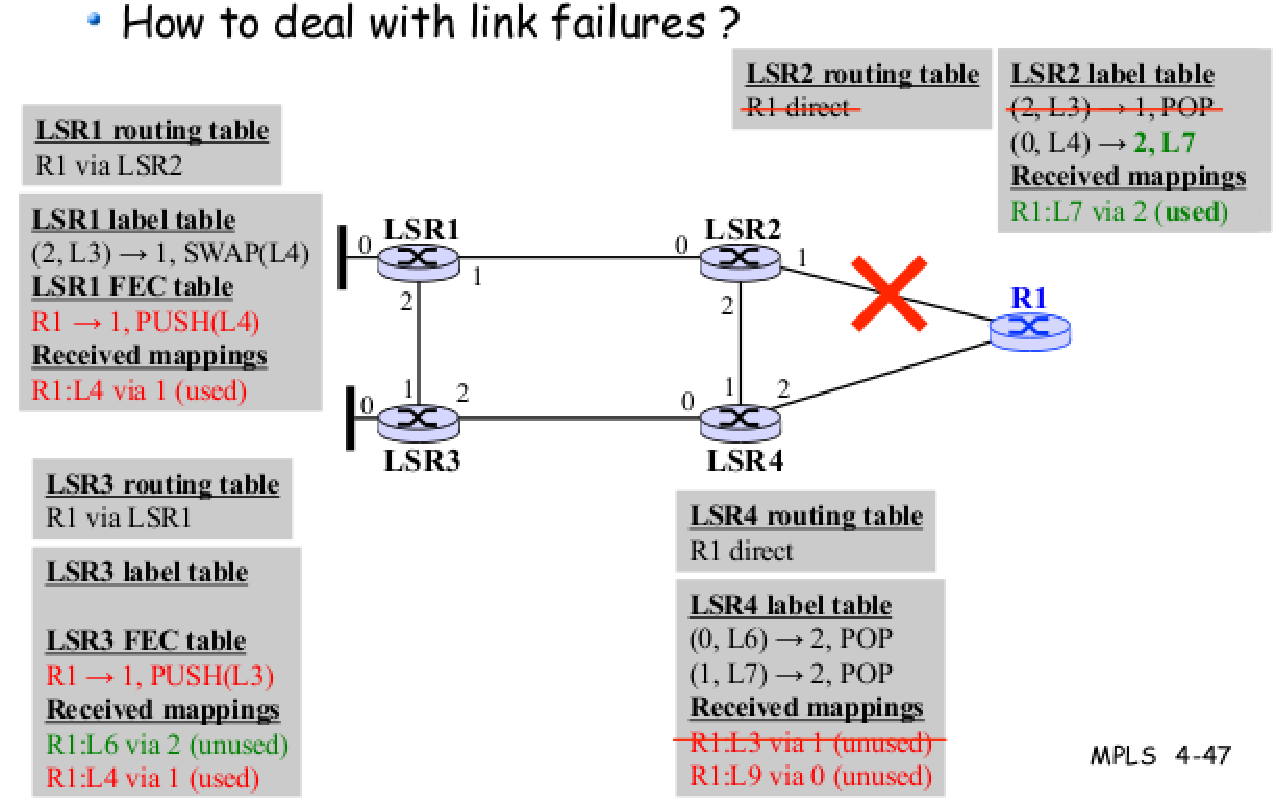
\includegraphics[width=200px]{img_020.pdf}
\end{center}	

\subsubsection*{Traffic Engineering}

L'idée est de développer un réseau IP normal ou IP+MPLS (pour que les paquets soient forwardés sur le plus court chemin). On
collecte ensuite des statistiques aux routeurs en bordure sur la charge du trafic afin d'identifier les parties les plus 
congestionnées du réseau. Ensuite les ingress LSR établiront des sessions LSP le long de chemins bien choisis pour amener 
certains flux en dehors des zones congestionnées. Cette approche soulève 2 questions. La première est de savoir comment établir
des sessions LSP avec des contraintes de qualité de service. Pour ce faire, on a besoin d'informations sur la capacité de 
chaque lien ainsi que d'un algorithme permettant de choisir le meilleur chemin en se basant sur ces contraintes. \\

\noindent Pour les informations, il faudrait ajouter deux choses aux protocoles de routage déjà existants : 
\begin{enumerate}
\item un moyen de distribuer l'information à propos de l'état courant;
\item un moyen de calculer un chemin sujet à des contraintes.
\end{enumerate}

\noindent Typiquement on va déployer celà sur des protocoles à état de lien tels que \textbf{OSPF} et \textbf{IS-IS}. En effet, 
il est difficile d'informer des routeurs de l'état des liens à distance dans des protocoles à vecteur de chemin/distance tels 
que \textbf{BGP} et \textbf{RIP}. De plus, avec les protocoles à état de lien :
\begin{itemize}
\item les routeurs coopèrent pour distribuer une carte du réseau $\rightarrow$ il devient simple d'ajouter de l'information à 
propos de la charge du réseau.
\item les routeurs distribuent des paquets d'état de lien avec des informations de charge
\begin{itemize}
\item[$\rightarrow$] le délai est déjà distribué comme la métrique IGP,
\item[$\rightarrow$] la bande passante/charge du lien est l'information principale à distribuer,
\item[$\rightarrow$] compromis entre la distribution fréquente et rare pour éviter la surcharge du réseau.
\end{itemize}
\end{itemize}

Le problème potentiel est le fait que les informations ne sont pas échangées immédiatement. Il se peut donc qu'un flot soit 
ajouté (ou du moins que l'on essaie de l'ajouter) sur un lien qui n'a plus assez de bande passante parce que le noeud n'a pas 
encore reçu l'information comme quoi il n'y avait plus assez de bande passante (cf Figure ci-dessous).

\begin{figure}[h!]
    \begin{center}
    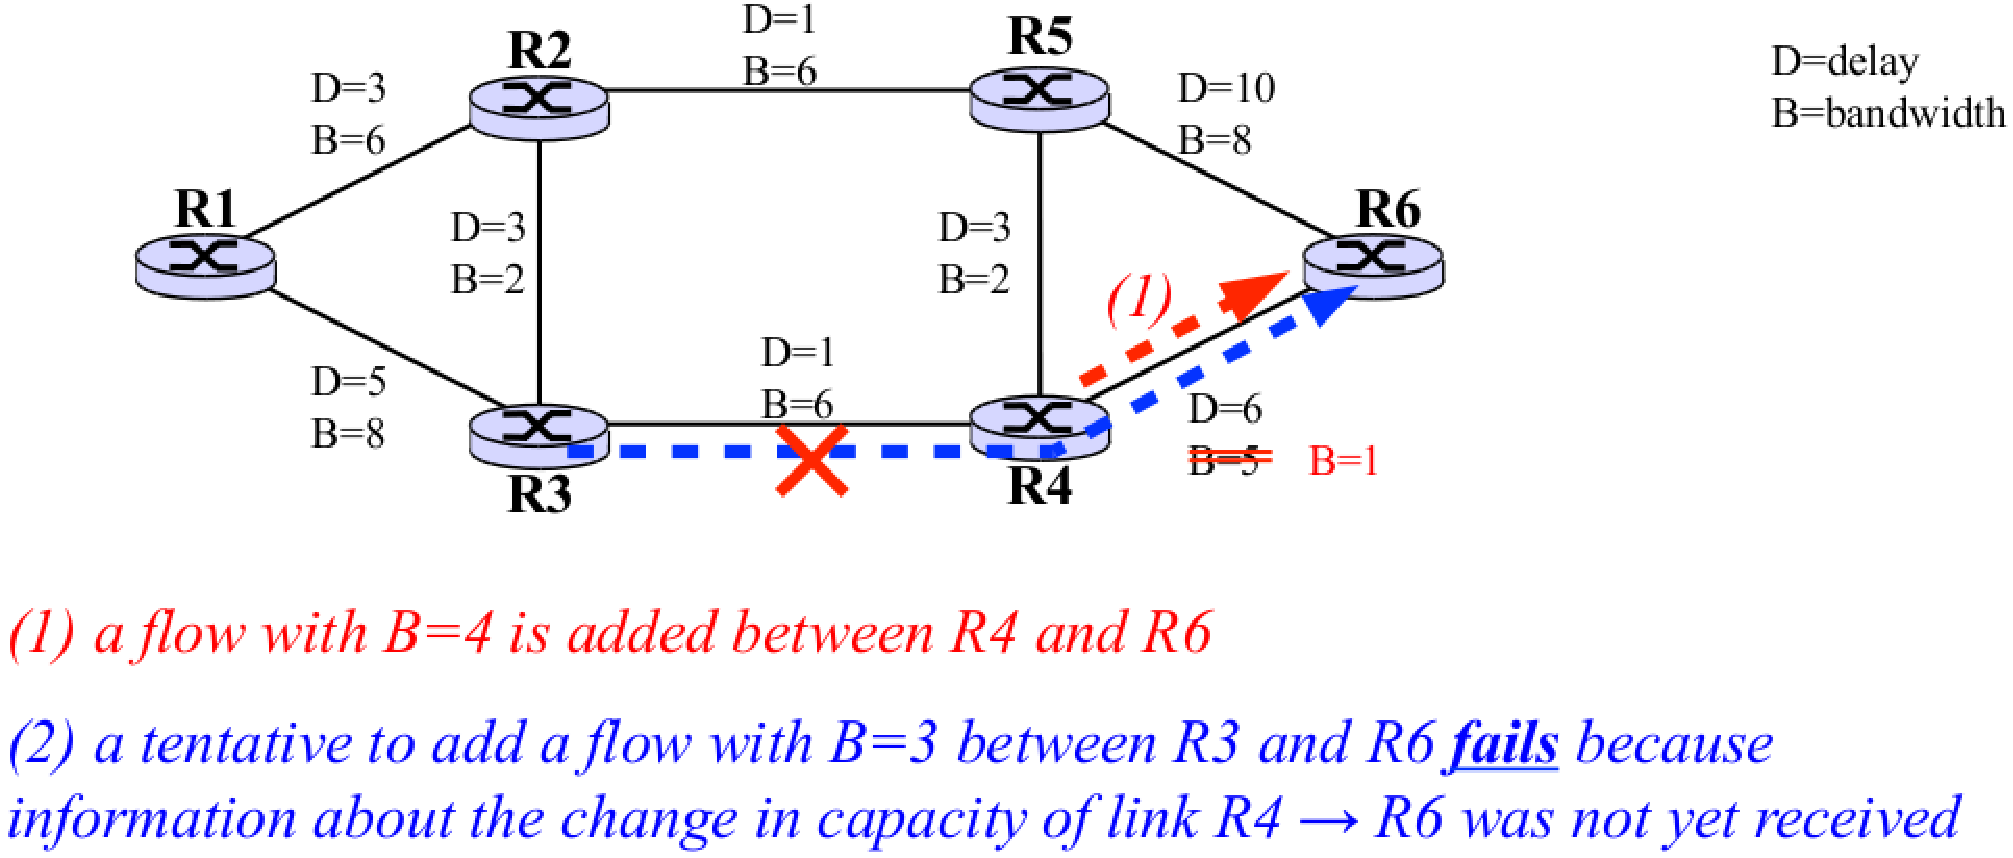
\includegraphics[width=250px]{img_021.pdf}
    \caption{Problème potentiel}
    \end{center}	
\end{figure}

Comment exprimer une contrainte ? Il y a 3 manières :
\begin{itemize}
\item \dblu{additive constraint} : trouver le(s) chemin(s) qui minimise(nt) $\sum{d_i}$ (comme pour le nombre de hop ou des 
délais ou couts des liens par exemple).
\item \dblu{multiplicative constraint} : trouver le(s) chemin(s) qui minimise(nt) $\prod{d_i}$ (comme pour le taux de perte par 
exemple)
\item \dblu{concave constraint} : trouver le(s) chemin(s) le(s) plus court(s) qui contiennent des liens qui respectent tous une 
contrainte donnée. (comme pour la bande passante par exemple)
\end{itemize}

Avec une seule contrainte additive ou multiplicative on utilise simplement Dijkstra, mais dès qu'il y a 2 ou plus de 
contraintes, le problème est NP-difficile. Heureusement, les contraintes concaves sont faciles à prendre en compte, il suffit 
simplement d'enlever les liens ne respectant pas la contrainte des choix possibles puis appliquer Dijkstra.

\begin{figure}[h!]
    \begin{center}
    \includegraphics[width=200px]{img_022.pdf}
    \caption{Application d'une contrainte concave}
    \end{center}	
\end{figure}

Par exemple ici on cherche à trouver le chemin le plus court ayant au moins 3Mbps de bande passante, on enlève donc les liens 
(croix bleue) qui ne peuvent procurer cette bande passante. \\

Plusieurs chercheurs ont proposés des solutions pour le routage avec contraintes et aujourd'hui on a tiré les leçons de ces
propositions :
\begin{itemize}
\item le routage avec contraintes doit être appliqué aux flux et non aux paquets un à un,
\item la bande passante et le délai sont des contraintes clés (le délai jitter est moins important et plus difficile à prendre 
en charge efficacement)
\item la sélection du chemin doit être fait par la source, aucun noeud du chemin ne prend de décision de routage. Si le flux 
envoyé sur le chemin n'est pas acceptable, la \textbf{source} devra en trouver(calculer) un autre.
\end{itemize}
Il existe des protocoles de routage avec contraintes, les plus connus sont $OSPF-TE$, $ISIS-TE$ et $PNNI$ ($ATM$). \\

Dans le cas de $OSPF-TE$, par exemple, les informations supplémentaires suivantes sont distribuées :
\begin{itemize}
\item le type de lien et son identifiant,
\item les adresses IP locale et distante,
\item la métrique de traffic engineering, qui est une métrique supplémentaire pour calculer les coûts des liens,
\item la bande passante maximale, 
\item la bande passante réservable maximale,
\item la bande passante non-réservée,
\item classe/couleur de la ressource (peut être utilisée pour définir le type du lien).
\end{itemize}

\subsubsection{RSVP}

Les objectifs de ce protocole sont de supporter l'établissement de flux unidirectionnel dans les réseaux IP. (il est approprié 
pour l'unicast et multicast IP). Ce protocole utilise principalement 2 messages importants :
\begin{enumerate}
\item \dblu{PATH} message envoyé par l'expéditeur aux routeurs et récepteurs pour informer du nouveau flux et des ressources 
qu'il requiert MAIS aucune ressource n'est réservée via ce message. Un état de chemin est tout de même garder dans les routeurs 
jalonnant le chemin, mais rien de plus.
\item \dred{RESV} message envoyé par les routeurs/récepteurs pour réserver les ressources pour le flux indiqué par le PATH. Ces 
messages remontent le chemin employé par le PATH, chemin qu'emploieront les datagrammes IP.
\end{enumerate}

Un paquet RSVP contient plusieurs objets, identifiés par un champ "Class-num" dans le header du même objet. Voici les quelques 
objets connus :
\begin{itemize}
\item \blu{SESSION} contient l'adresse IP de destination, le protocole IP et le port de destination,
\item \blu{SENDER\_TEMPLATE} utilisé pour identifier l'expéditeur via son adresse IP et optionnellement le port,
\item \blu{RSVP\_HOP} contient le hop précédent et le next-hop,
\item \blu{SENDER\_TSPEC} définit les caractéristiques de traffic du flux.
\end{itemize}

\begin{figure}[h!]
    \begin{center}
    \includegraphics[width=350px]{img_023.pdf}
    \caption{Un exemple de RSVP}
    \end{center}	
\end{figure}

Les routeurs RSVP tiennent en mémoire un état par flux. Il est possible de gérer cet état de 2 façons :
\begin{enumerate}
\item de manière \rouge{hard state}, c'est-à-dire que l'état est créé à l'établissement du flux et supprimé quand ce flux est 
enlevé. Si un routeur intermédiaire crash, les réservations et l'état sont perdus. Cette solution est employée dans la plupart 
dans les réseaux "circuit-switched".
\item de manière \rouge{soft state}, c'est-à-dire qu'à l'état est associé un timer et quand celui-ci tombe à 0, l'état est 
supprimé. Les hôtes doivent alors s'échanger des PATH/RESV de manière périodique et si un routeur intermédiaire crash ou que le
chemin change, l'état est automatiquement retiré. \\
\end{enumerate}

RSVP utilise le \rouge{soft state}.

\subsubsection{RSVP-TE}

Il s'agit de l'extension de RSVP pour MPLS. Les ingress LSR envoient des messages \blu{PATH} \textit{(qui incluent un Label 
Request Object)} vers les egress LSR. Ceux-ci répondent par des messages \rouge{RESV} qui va propager le label à employer de 
hop en hop.

\begin{figure}[h!]
    \begin{center}
    \includegraphics[width=350px]{img_024.pdf}
    \caption{Exemple d'établissement de session LSP avec RSVP-TE}
    \end{center}	
\end{figure}

Il est également possible d'établir ces sessions sur d'autres liens que les plus court. L'ingress LSR peut spécifier la route à
emprunter pour établir le LSP via un \textbf{ERO}\textit{(Explicit Route Object)} (dans le message \blu{PATH}). Cet objet 
contient une liste d'adresses IP, de préfixes de sous-réseau et de numéro d'AS. Il y a 2 types de routes :
\begin{enumerate}
\item \rouge{Strict route}, route dont chaque LSR spécifié \textbf{doit} être visité et uniquement ceux-là.
\item \rouge{Loose route}, route dont chaque LSR spécifié \textbf{doit} être visité mais où le LSP peut passer par un autre
LSR entre 2 LSR's spécifiés.
\end{enumerate}

\begin{figure}[h!]
    \begin{center}
    \includegraphics[width=300px]{img_025.pdf}
    \caption{Exemple d'emploi du ERO.}
    \end{center}	
\end{figure}

\noindent \underline{\textbf{Problèmes à considérer}}\\

\noindent
\begin{itemize}
\item Pour réserver la bande passante il faut utiliser le \textit{Tspec} et le \textit{Rspec} $\Rightarrow$ \gre{Résolu}.
\item Pour supporter des flux de trafic variable, il doit être possible de modifier les ressources du LSP dynamiquement et s'il
n'y a pas assez de ressources disponibles, que le LSP conserve les anciennes ressources.
\item Comment changer dynamiquement la route employée ? (meilleur bande passante ailleurs ou un lien qui tombe dans la route 
actuelle)
\end{itemize}

\section{Réseau de capteurs sans fil (Wireless Sensor Network - WSN)}
\subsection{Motivations}
\subsubsection{Tentative de définition}
\begin{itemize}
\item Large quantité de noeuds-capteurs bon-marchés, peu gourmands en énergie
  et multi-fonctionnels déployés dans une région à intérêt.
\item Capables de calculs
\item Communiquent sur courte distance
\item Collaborent entre eux pour accomplir des tâches communes
\end{itemize}

\subsubsection{Exemple d'applications}
réseaux intelligents, cités intelligentes, agriculture, construction,
industrie, sécurité, santé, informatique portable, ...

\subsubsection{Plus qu'un simple réseau sans fil}
\begin{itemize}
\item Densité de noeuds plus élevée
\item Contraintes plus grandes: énergie, stockage et calculs limités
\item Auto-configurable
\item Applications spécifiques: différent des applications d'un simple PC
\item Manque de fiabilité plus élevé: changements de topologie fréquents
\item Trafic de plusieurs noeuds vers un seul noeud (many-to-one traffic),
  de la source vers le puît.
\end{itemize}

\subsubsection{Composition principale d'un WSN}
\begin{itemize}
\item Miniaturisation du matériel
\item Environnement de communication changeant:
  sans-fil avec perte et pas toujours allumé, besoin d'une nouvelle pile
  de protocoles réseau (routage, communication, ...)
\item Application: temps réel requis, duty cycle, ressources limitées,
  informatique embarquée, tolérant aux défaillances du capteur
\item Comportement adaptatif: condition de communication changeantes,
  environnement changeant, ...
\end{itemize}

\subsection{Noeud-capteur}
\subsubsection{Structure typique d'un noeud capteur}
\includegraphics[width=0.75\textwidth]{sensor_struct}

\subsubsection{Matériel typique d'un noeud capteur}
\begin{itemize}
\item Processeur/microcontrolleur limité:
  lent (8 bits data path), basse fréquence (8MHz), pas d'opération à virgule
  flottante, pas de cache, pas d'unité de gestion mémoire, pas de MPU \textit{(Memory Protecting Unit)},
  pas d'instruction en pipeline.
\item Mémoire limitée:
  50KB de mémoire flash (pour le programme), 5-10 KB (pour la RAM)
\item Radio de faible puissance:
  50-100m de portée, non fiable, consomme quand même beaucoup d'énergie
  ($\sim 20mA$), débit de $100-200 Kbps$
\item Alimentation limitée:
  utilisation de batterie, énergie solaire, vibration des récoltes, ...
  (piles AA: $2500mAh$, soleil: $5mA/cm^3$)
\end{itemize}

\subsubsection{Architecture d'un noeud capteur}
\begin{itemize}
\item Exemple de radio: (voir slide 12)

\item Exemple de capteur:
  \begin{itemize}
  \item Passif:
    lumière, son;
    humidité, pression, température;
    vitesse angulaire/linéaire;
    vibration, tension d'un matériel;
    sensible à une substance chimique;
    détecteur de fumée;
    caméra; ...
  \item Actif:
    sonar, radar, sismique, ...
  \item Actionneur:
    LED, relais, moteur, ...
  \end{itemize}

\item Exemple de source d'énergie
  \begin{itemize}
  \item Énergie stockée: piles (non) rechargeables
  \item Énergie captée:
    photovoltaïque, variation de température/pression, vibrations,
    flux d'air/de liquide
  \item Métriques (en énergie par volume - $J/cm^3$):
    piles rechargeables: $200mWh/cm^3$,
    soleil: $15mW/cm^3$,
    vibrations: $0.01-0.1 mW/cm^3$
  \end{itemize}
\end{itemize}

\subsubsection{Consommation d'énergie - Microcontrôleur}
Utilisation de techniques pour une consommation d'énergie efficace.
Trois états possibles:
\begin{itemize}
\item actif: mode de fonctionnement normal, consommation max
\item attente: fréquence du processeur faible, certains périphériques éteints
\item repos: pas en fonctionnement mais fréquence basse, timer pour réveil
\end{itemize}
Mais les transitions entre les états ne sont pas libres car elles nécessitent
de l'énergie. Plus l'état de repos est profond, plus il faudra d'énergie pour
l'en sortir. Alors quand cela vaut-il la peine de changer d'état ?
\\\\
\underline{Exemple}:
Supposons qu'au temps $t_1$, il n'y a rien à faire avant $t_{event}$.
Faut-il aller dormir ou pas ?
Aller dormir demande un temps $\tau_{down}$ et se réveiller $\tau_{up}$.
La consommation d'énergie vaut $P_{active}$ si l'état est actif, et
$P_{sleep}$ au repos.
\includegraphics[width=0.75\textwidth]{consumption1}

\begin{itemize}
\item Si on reste actif : $E_{active} = \tau_{idle} \times P_{active}$
\item Si on passe en mode repos :
  $E_{sleep} = \tau_{down} \times \frac{P_{active} + P_{sleep}}{2} +
  (\tau_{idle}-\tau_{down}) \times P_{sleep}$
\end{itemize}
\includegraphics[width=0.75\textwidth]{consumption2}

$$\begin{array}{rcl}
E_{saved} & = & E_{active} - E_{sleep} \\
        & = & \tau_{idle} \times P_{active} -
              (\tau_{down} \times \frac{P_{active} + P_{sleep}}{2} +
              (\tau_{idle} - \tau_{down}) \times P_{sleep}) \\
        & = & \tau_{idle} \times (P_{active} - P_{sleep}) - \tau_{down} \times
              \frac{P_{active} + P_{sleep}}{2}\\
E_{overhead} & = & \tau_{up} \times \frac{P_{active} + P_{sleep}}{2}
\end{array}$$

\includegraphics[width=0.75\textwidth]{consumption3}

Partir au repos si $E_{overhead} < E_{saved}$
càd lorsque:

$$\begin{array}{rcl}
  \tau_{up} \times \frac{P_{active} + P_{sleep}}{2} & < &
  \tau_{idle} \times (P_{active}-P_{sleep})-\tau_{down} \times
  \frac{P_{active} + P_{sleep}}{2}\\
  & \Updownarrow & \\
  t_{event} - t_1 & > & \frac{1}{2}(\tau_{down} +
  \frac{P_{active} + P_{sleep}}{P_{active} - P_{sleep}} \times \tau_{up})
\end{array}$$

\subsubsection{Consommation d'énergie - Radio}
Une radio peut aussi se trouver dans différents états:
\begin{itemize}
\item transmission:
  émetteur-récepteur actif, antennes émettent de l'énergie
\item réception:
  émetteur actif, réception en cours, amplificateur LNA consomme une
  grande partie de l'énergie
\item attente:
  prêt à recevoir, pas de réception en cours, récepteur actif (LNA aussi),
  consommation d'énergie équivalente à l'état réception
\item repos:
  plupart des émetteurs-récepteurs éteints (prend un certain temps à rallumer),
  difficile à uniquement allumer lors d'une réception
\end{itemize}

Il est possible d'adapter la puissance de l'émetteur, mais l'énergie consommée
par l'émetteur n'est pas directement proportionnelle à celle produite par
l'antenne (sous forme d'ondes).
Donc réduire la puissance de l'émetteur ne permettra pas une
forte diminution de l'énergie consommée.

Du côté du récepteur, peu de changements possibles. On peut éventuellement
aller au repos quand c'est possible. Implique l'utilisation d'un cycle avec
une période active pour écouter les autres noeuds et une période de repos
lorsqu'on ne fait rien (\textit{duty cycle}).

\subsection{Architecture d'un réseau de capteurs}
\includegraphics[width=0.75\textwidth]{network_archi}

Différentes approches pour accéder à un noeud:
\begin{itemize}
\item single-hop: se fait sur longue distance, ce qui implique un haut
  coût de transmission (énergie augmente exponentiellement avec la distance).

  \includegraphics[width=0.75\textwidth]{network_archi1}
\item multi-hop: chaque noeud a le même rôle et peut forwarder une donnée
  d'un pair vers le puît sur des chemins multi-hop
  $\Rightarrow$ diminution de la distance de transmission.

  \includegraphics[width=0.75\textwidth]{network_archi2}
\item clustering: ensemble de noeuds regroupés dans un cluster,
  des noeuds-puît rassemblent le trafic des clusters, le noeud principal
  d'un cluster envoit les données au puît principal
  $\Rightarrow$ noeuds-puît doivent être plus puissants
  mais moins de perte d'énergie.

  \includegraphics[width=0.75\textwidth]{network_archi3}
\end{itemize}

\subsection{Couche MAC}
\subsubsection{Protocoles MAC traditionnels}
\begin{itemize}
\item On ne peut pas utiliser CSMA/CD (collision detection)
  car cela suppose que l'émetteur puisse détecter les collisions
  $\rightarrow$ utilisation de CSMA/CA (collision avoidance).
\item Les problèmes du terminal caché et des terminaux exposés sont règlés par
  l'utilisation de RTS/CTS mais ceux-ci introduisent un overhead significatif.
\item Pourquoi ne pas utiliser des protocoles existants (Bluetooth, 802.11) ?
  Car le Bluetooth a besoin d'un maître permanent pour le polling et
  le 802.11 demande d'être constamment en écoute.
\end{itemize}

\subsubsection{Contraintes demandées par le protocole MAC}
\begin{itemize}
\item Doit conserver l'énergie: très différent des traditionnels WLAN.
\item Extensible et robuste par rapport aux changements fréquents de topologie:
  noeud éteint temporairement, mobilité, déploiement de nouveaux noeuds,
  morts de noeuds existants.
\end{itemize}

\underline{Problèmes d'énergie}
\begin{itemize}
\item Collisions:
  coûts de réception inutiles à la destination,
  coûts de transmission inutiles à la source. Éviter les collisions
  le plus possible.
\item Overhearing:
  le réseau sans-fil s'appuie sur le broadcast, beaucoup de noeuds
  reçoivent des messages qui ne leur sont pas destinés et qu'ils droppent.
\item Overhead du protocole:
  Contrôle de frame lié à MAC, header de paquets.
\item Écoute en mode attente:
  consomme une énergie significative $\rightarrow$ aller au repos (duty cycle).
\end{itemize}

\subsubsection{Différents protocoles MAC}
\begin{itemize}
\item basés sur les conflits: CSMA protocols, S-MAC, Mediation device protocol
\item basé sur un planning: LEACH, SMACS, TRAMA
\item hybride: B-MAC, Z-MAC
\end{itemize}
On étudiera ici les protocoles S-MAC et Mediation device ainsi qu'un
cas d'étude: le IEEE 802.15.4.

\subsubsection{S(ensor)-MAC}
\underline{Objectifs}:
\begin{itemize}
\item minimiser les conflits:
  utilisation d'un schéma CSMA/CA pour le broadcast et d'un schéma CSMA/CA
  avec RTS/CTS/DATA/ACK pour l'unicast.
\item minimiser l'attente d'écoute:
  utilisation d'un duty cycle faible càd courte période d'écoute et longue
  période de repos.
\item overhearing: les noeuds peuvent se reposer dès qu'ils entendent un RTS
  pour un autre noeud, chaque paquet indique la taille de transmission pour
  que les autres noeuds sachent quand se réveiller.
\end{itemize}

\underline{Schéma de réveil périodique}:
Un noeud alterne entre des périodes d'écoute et de repos selon son
planning (schedule). La période d'écoute peut servir à la réception et
la transmission. L'objectif de S-MAC est donc de tenter de coordonner
le planning des différents voisins pour que leurs périodes d'écoute commencent
au même moment.

Une période d'écoute est divisée en 3 phases: SYNC, RTS et CTS.

\includegraphics[width=0.75\textwidth]{smac_periods}

\begin{itemize}
\item SYNC:
Le noeud accepte les paquets SYNC de ses voisins. Les voisins y notifient
leur table de planning. Pendant la période de SYNC un schéma slotted CSMA/CA
est utilisé (comme pour 802.11).
Un paquet SYNC contient l'ID de l'envoyeur et le moment de son prochain repos.

Un noeud qui veut transmettre durant la période de SYNC choisit un slot
aléatoirement, vérifie si le canal est libre et commence à transmettre.
Si le canal n'est pas libre, le noeud fait marche arrière jusqu'à la prochaine
période de SYNC.
Un noeud doit envoyer sa table de planning périodiquement mais pas
à chaque réveil.
\item RTS:
Le noeud écoute les RTS de ses voisins (la canal est partagé en utilisant
slotted-CSMA/CA comme pour SYNC).
\item CTS:
Le noeud transmet un CTS si un RTS a été reçu.
\end{itemize}

\vspace{10px}
\underline{Synchronisation}:
Vouloir une synchronisation à l'échelle du réseau est difficile et peut
augmenter la contention (tous les noeuds se réveillent en même temps et
se disputent un nombre limité de slots).
Solution: utilisation de clusters virtuels càd des groupes de noeuds qui
partagent le même planning.

Au départ, un noeud qui s'allume écoute ses voisins. S'il reçoit un planning
d'un voisin, il l'adopte comme son planning et en informe ses voisins par
broadcast. Sinon, il choisit un planning aléatoire.
Les noeuds qui ont le même planning appartiennent au même cluster.
Si un noeud a choisit son propre planning, qu'aucun voisin n'a adopté son
planning et qu'il reçoit un planning d'un voisin, il adopte ce nouveau
planning.
(exemple concret voir slides 45-50).

\underline{Limiter l'overhearing}:
Les noeuds vont au repos dès qu'ils reçoivent un RTS pour un autre noeud.
Chaque paquet indique la taille de la transmission pour qu'un noeud sache
quand se réveiller. Mais quels noeuds doivent aller au repos ?
Les voisins du récepteur et de l'envoyeur.

\includegraphics[width=0.75\textwidth]{smac_overhearing}

\underline{Résumé S-MAC}:
\begin{itemize}
\item Avantages: Les noeuds peuvent passer plus de temps au repos.
\item Inconvénients: Utilisé avec un protocole de routage en maille,
  la latence peut être élevée car il faut attendre que les noeuds
  de la route se réveillent. La latence subie est d'à peu près
  $N \times T_{sleep}$ où $N$ est le nombre de hops et $T_{sleep}$
  la période de repos.
\item Améliorations possibles:
  Utilisation d'une écoute adaptative (adaptive-listening).
  Un noeud du next-hop peut plannifier une période supplémentaire
  d'écoute pour pouvoir écouter le RTS de son prédécesseur sur le chemin.
\end{itemize}

\subsubsection{Mediation device protocol}
Il n'y a pas de temps de référence global, chaque noeud peut avoir
ses propres planning de repos.
Le principe se présente comme suit:
\begin{itemize}
\item Quand un noeud se réveille, il transmet une courte requête ``balise''
  (query beacon)
  indiquant qu'il est voulu de recevoir les paquets des autres.
\item Ensuite, il reste éveillé pour un court moment, et si aucun paquet
  n'est reçu, il retourne au repos.
\item Si un noeud veut transmettre un paquet à un voisin, il doit se
  synchronisé avec lui.
\item Mediation device autorise les noeuds à se synchroniser sans devoir
  rester éveillé pendant un long moment.
\end{itemize}

\vspace{5px}
\includegraphics[width=0.75\textwidth]{mediation_device_protocole}
\vspace{5px}

\underline{Avantages}:
\begin{itemize}
\item Pas besoin de synchronisation globale.
\item La plupart de l'énergie est envoyée au dispositif de médiation.
\end{itemize}

\underline{Inconvénients}:
\begin{itemize}
\item Nécessite un \textit{mediation device} réactif à l'énergie
\item Si plusieurs noeuds prennent le même planning, ils pourraient envoyer
  leur requête ``balise'' en même temps $\rightarrow$ collisions.
\end{itemize}

\underline{Travail supplémentaire}:
\begin{itemize}
\item Réordonnancer les messages dans le cas de collisions répétées.
\item Mediation device protocol distribué.
\end{itemize}

\subsubsection{IEEE 802.15.4}
Utilisation des couches physiques et MAC d'un réseau sans-fil personnel (WPAN)
à bas débit.

\underline{Caractéristiques}:
\begin{itemize}
\item Moyen à bas débits
\item Dans les groupes industriels/scientifiques/médicaux
\item Autorise les schémas basés sur la contention et la plannification
\end{itemize}

\underline{Architecture}:
Deux types de noeuds: les Full Function Device (FFD) qui peuvent travailler
comme un coordinateur de réseau personnel (PAN), un simple coordinateur ou
un device; et les Reduced Function Device (RFD) qui sont de simples devices.

La topologie du réseau peut être en étoile pour connecter les devices au
coordinateur ou en P2P pour connecter les coordinateurs entre-eux.

\includegraphics[width=0.75\textwidth]{ieee802154_topology}

\underline{Adressage}:
Chaque noeud a une adresse unique codée sur 64 bits. Les premiers 24 bits
représentent l'ID unique de l'organisation (OUI) alouée au fabricant par
IEEE. Et les 40 bits suivants sont assignés par le fabricant.

Les noeuds peuvent aussi utiliser un adressage 16-bits pour diminuer
l'overhead. Mais les adresses courtes ont une portée plus limitée et peuvent
uniquement être utilisées dans un même PAN.
Donc, les devices souhaitant atteindre un PAN extérieur le feront
avec leur adresse courte + l'ID de destination du PAN externe
(32 bits au total).

\underline{Format des frames}:

\includegraphics[width=0.75\textwidth]{ieee802154_frame}

\underline{Rôle du coordinateur}:
\begin{itemize}
\item Gérer la list des devices associés (association requête/réponse MAC
  command frame, utilisation des adresses 64-bits)
\item Allouer une adresse courte aux devices
\item Gérer la transmission des frames ``balise'' (beacon)
\item Allouer un time slot garanti (GTS) en mode beaconed
\end{itemize}

\underline{Superframe}:
Le standard spécifie un mode \textit{beaconed} où les canaux d'accès sont
organisés par un coordinateur. Le beacon envoyé sur base régulière marque le
début d'une superframe.
La période active est divisée en 16 slots. Le premier est le beacon,
le reste est réparti entre CAP \textit{(Contention Access Period)} et GTS.
Le coordinateur doit être actif durant toute la période active.

\includegraphics[width=0.75\textwidth]{ieee802154_superframe}

\underline{Accès au média durant CAP (contention possible)}:
Utilisation du protocole \textit{slotted CSMA/CA} (synchronisation
avec beacon). Chaque slot CAP est divisé en périodes de backoff.

\underline{Accès au média durant CFP (garanti sans contention)}:
Utilisation de TDMA (Time Division Multiple Access) (synchronisation
avec beacon). Avant d'accéder au média durant le période CFP, un noeud doit
faire une requête d'un time slot au coordinateur.
La requête GTS contient le nombre de slots demandés, la direction (transmission
ou réception) et indique s'il s'agit d'une requête d'allocation ou
de désallocation.
La fenêtre beacon contient la liste des adresses courtes qui sont autorisées
à utiliser leur GTS pendant la période CFP de la superframe.

\includegraphics[width=0.75\textwidth]{ieee802154_gts}


\subsection{Couche réseau}
\subsubsection{Introduction}
\underline{Objectif}:
La couche 3 fournit des chemins multi-hop. Beaucoup d'approches différentes
sont possibles. On voit ici le protocole de routage MANET
(Mobile Ad-hoc Network):
\begin{itemize}
\item Divisé en protocole dirigé par des tables et des protocoles à la demande
\item Optimized Link-State Routing (OLSR)
\item Ad-hoc On-demand Distance Vector (AODV)
\end{itemize}

\subsubsection{Ad-hoc On-demand Distance Vector (AODV)}
\underline{Caractéristiques}:
\begin{itemize}
\item Protocole de routage pour réseaux maillés.
\item Fonctionne au dessus de IP, utilise UDP avec port 654
\item Peut être utilisé sur des réseaux avec ou sans-fil
\item 4 types de messages:
  Route Request (RREQ), Route Reply (RREP), Route Error (RERR) et
  Route-Reply Acknowledgment (RREP-ACK)
\item Pas spécifique aux WSN
\item Implémentation disponible dans TinyOS et Contiki
\end{itemize}

\underline{Fonctionnement}: (slides 70-80)\\
Si un noeud veut communiquer avec un autre noeud hors d'atteinte:
\begin{itemize}
\item Le noeud envoie un RREQ en broadcast.
\item Les noeuds qui le reçoivent mettent à jour leur table de routage
  avec une entrée pour le dernier envoyeur du message et le créateur du
  message.
\item Ils broadcastent à leur tour le RREQ.
\item Quand le noeud destination reçoit le RREQ, il met à jour sa table
  de routage et renvoie un RREP en unicast.
\end{itemize}

\underline{Détails supplémentaires}
\begin{itemize}
\item Recherche en cercle: RREQ envoyé avec un TTL. Si aucune réponse,
  renvoie avec un TTL plus élevé.
\item Mécanismes de flooding: Utilisé pour le broadcast des RREQ. Un noeud
  garde la trace du numéro de séquence du créateur du message dans le RREQ.
  Si un autre RREQ du même créateur est reçu, il est forwardé si le numéro
  de séquence est plus grand que l'ancien, il est jeté sinon.
\item Limite du flooding: Un noeud qui reçoit un message RREQ et qui
  a déjà une entrée pour la destination dans sa table de routage et
  dont le numéro de séquence de l'entrée est $\geq$ au numéro de séquence du
  RREQ, alors le noeud répond avec un message RREP et ne forwarde pas le RREQ.
\item Défaillance du lien: Des \textit{Hello messages} sont envoyés
  régulièrement par un noeud sur une route active vers ses prédécesseurs.
  Si aucun \textit{Hello} n'est reçu dans un certain laps de temps, la route
  est considérée comme invalide et une procédure de recovery doit être lancée.
\end{itemize}

\subsection{Couche transport}
\underline{TCP pour WSNs} ?
TCP a été conçu pour les réseaux filaires qui ont un faible taux de perte de
paquets dû aux erreurs, et un haut taux de perte de paquets dû à la congestion.
\begin{itemize}
\item Perte de paquet interprétée comme congestion $\rightarrow$
  réduction de la fenêtre de congestion $\rightarrow$ réduction du débit.
\item Principe de end-to-end $\rightarrow$ considère que les noeuds
  intermédiaires sont muets et ne peuvent pas prendre part à une retransmission.
\end{itemize}

\underline{Problèmes avec TCP}:
\begin{itemize}
\item Ne fonctionne pas bien avec les réseaux sans fil à cause du haut taux
  d'erreur (Bit Error Rate)
  \begin{itemize}
  \item paquets perdus à cause d'erreur de bit: 5-10\% au plus
  \item paquets perdus impliquent une retransmission et réduction de la fenêtre
    de congestion malgré qu'il n'y ait pas de congestion
  \item les paquets peuvent être retransmis par la couche lien mais cela
    augmente le RTT $\rightarrow$ augmente le RTO $\rightarrow$
    TCP réagit lentement aux changements de congestion.
  \item injustice augmentée:
    les plus longs chemins ont une plus grande probabibité d'erreur
    $\rightarrow$ dégradation des performances
  \item ...
  \end{itemize}
\item Les retransmissions TCP ent-to-end sont nuisibles pour la contrainte
énergétique des WSN car plusieurs noeuds pourraient avoir besoin de
retransmettre sur un chemin multi-path.
\end{itemize}

\underline{Solution proposée}:
\begin{itemize}
\item Amélioration de TCP avec des liens sans-fil:
  split connections (\textcolor{blue}{I-TCP}, Split-TCP),
  solution de la couche lien (Snoop)
\item Amélioration de TCP dans les WSNs:
  Distributed Caching Protocol (\textcolor{blue}{DCP})
\item Autres protocoles de transport: pas vu ici
\end{itemize}

\underline{\bf Split connection (I-TCP)}:
\begin{itemize}
\item \underline{Idée de base}:
  La connection TCP est splittée à la station de base (BS),
  ensuite, deux connexions sont établies et la BS copie d'une
  connexion à l'autre.

  \includegraphics[width=0.75\textwidth]{wsn_itcp}
\item \underline{Avantages}:
  repose exactement sur le même protocole TCP,
  petits RTT pour chaque connexion (recovery plus rapide),
  les pertes sans-fil sont cachées de la connexion entre BS et FH,
  et la connexion entre MH et BS peut utiliser un protocole de transport
  affiné.
\item \underline{Inconvénients}:
  Viole le principe \textit{end-to-end} de TCP,
  de la mémoire et du CPU supplémentaire sont requis à la BS (buffer des 2 conn,
  controle de conn*2 et copie d'une conn à l'autre),
  et transfert plus complexe (nécessite un état à changer de la BS de base à
  la nouvelle BS).
\end{itemize}

\underline{\bf Distributed Caching Protocole (DCP)}:
\begin{itemize}
\item \underline{Idée de base}:
  Implique les noeuds intermédiaires le long d'un chemin
  multi-hop. Essaye de réaliser des retransmissions locales autant que possible.
  Repose sur des connaissances positives de la couche lien pour sélectionner
  ce qui doit être mis en cache.
\item Principe de fonctionnement:
  Chaque noeud doit être capable de mettre en cache quelques segments TCP.
  Met en cache les segments de haut num de séq.
  Vérrouille les segments en cache qui sont un-ack'd.
  soft-state dans les noeuds intermédiaires

  \includegraphics[width=0.75\textwidth]{wsn_dcp}
\item \underline{Avantages}:
  la retransmission se passe plus près de la destination $\rightarrow$
  celle-ci n'implique pas tous les noeuds du chemin multi-hop.
\item \underline{Inconvénients}:
  Les noeuds intermédiaires ont besoin de mémoire additionnelle pour
  mettre en cache les segments et les opérations supplémentaires.
  Difficulté de prédire les améliorations en présence de faible cache et
  d'une large fenêtre d'envoi (besoin de simulations/mesures expérimentales).
\end{itemize}

\subsection{Modèle de programmation / RTOS (real-time operating system)}
\subsubsection{Objectifs}
\begin{itemize}
\item Comprendre comment la programmation des systèmes embarqués en réseaux
  diffère de la programmation logicielle ordinaire (pas d'OS de support,
  programmation séquentielle vs événementielle).
\item Découvrir comment une pile IP peut tenir dans un très petit système
  (uIP/lwIP).
\item Avoir un contact avec les WSN récents orientés RTOS
  (TinyOS/nesC, Contiki/Protothreads)
\end{itemize}

\subsubsection{Différence avec la programmation ordinaire}
\underline{OS de support}
La programmation logicielle traditionnelle repose fortement sur les services
apportés par l'OS:
\begin{itemize}
\item contrôle/protection des accès aux ressources
\item gestion de l'allocation des ressources à différents utilisateurs
\item support pour les exécutions concurrentielles de pls processus
\item communication entre processus
\end{itemize}

Exigences des noeuds WSN:
\begin{itemize}
\item Les microcontrôleurs n'ont généralement pas assez de ressources pour
  accueillir un OS complet (pas de MMU \textit{(Memory Management Unit)}, mémoire limitée, ...).
\item Les exigences pour la concurrence sont différentes (unique user,
  multiples tâches).
\item Le peu de mémoire nécéssite souvent des schémas d'allocations statiques
  ou dynamiques.
\end{itemize}

\underline{Programmation séquentielle}
Les applications traditionnelles sont souvent conçues autour d'un modèle
de programmation séquentielle. Ce modèle pourrait mener à des pertes
au niveau des capteurs de données ou de la radio.

\underline{Processus basé sur la concurrence}:
Un OS fait attention au partage CPU et fournit un environnement d'exécution
en parallèle. Chaque processus a sa propre pile (WSN: pas approprié
à cause des contraintes mémoire) et le context-switching induit un overhead
significatif (WSN: consommation de CPU/énergie + risque de perte de données
au niveau du capteur et de la radio).

\underline{Programmation basée sur les événements}:
Insère la nature réactive des noeuds WSN dans le modèle de programmation.

\includegraphics[width=0.75\textwidth]{wsn_eventprog}

Principes de fonctionnement:
\begin{itemize}
\item boucle d'attente: ne fait rien, va au repos si nécessaire
\item gestionnaire d'événement:
  traite rapidement l'event entrant (donnée du capteur
  dispo, paquet entrant, ...), stocke les infos requises pour les traiter
  plus tard).
\item un gestionnaire d'event peut interrompre tout code normal
\item un gestionnaire d'event ne peut pas interrompre un autre gestionnaire
  (nécessiterait des coûts de context-switch - sauver piles et registres)
\item le gestionnaire d'event tourne jusqu'à son achevement.
\end{itemize}
Il y a ainsi seulement deux contextes d'exécution:
\begin{itemize}
\item un pour les gestionnaires d'event à temps critique (sans interrupt)
\item un pour le code normal (peut être interrompu)
\end{itemize}

\subsubsection{Pile IP - uIP}
\underline{Introdution}:
On a longtemps cru que IP était trop complexe et trop lourd pour être utilisé
dans les petits systèmes embarqués en réseau (MCU limité...).
Cette conviction a changé en 2001 avec la première version d'un prototype
d'une pile IP complète pour un MCU 8-bits (inclus IP, ICMP, TCP, UDP).

\includegraphics[width=0.75\textwidth]{wsn_uip}

\underline{Principes de fonctionnement}:
Arrivée de fenêtres de traitement du \textit{Communication device driver}, et
de paquets des applications. Réalise un traitement périodique.
\begin{itemize}
\item Traitement d'une entrée IP:
  \begin{itemize}
  \item vérifie la version (supporte v4/v6)
  \item vérifie la taille du header IP vis-à-vis de la taille de la frame reçue
  \item vérifie le flag de fragmentation (pour v4): si c'est un fragment
    alors il faut le copier dans le buffer de défragmentation, si ce buffer
    contient un datagramme IP complet alors continuer le traitement
    (pour v6 voir headers d'extension)
  \item vérifie l'adresse source: jette les adresses illégales
    (source=broad/multicast)
  \item vérifie l'adresse destination: distinction entre livraison locale et
    forwarding
  \item vérifie la checksum du header (v4)
  \item traite les headers d'extension (v6)
  \end{itemize}
\item Traitement d'une entrée ICMP:
  \begin{itemize}
  \item pour v4: uIP supporte seulement les message ICMP echo et va répondre
    avec un echo de réponse ICMP correspondant.
  \item pour v6: uIP supporte la découverte de voisins (messages NS/NA),
    la découverte de router (messages RS/RA), la détection d'adresse dupliquée,
    ...
  \end{itemize}
\item Traitement d'une entrée UDP:
  \begin{itemize}
  \item vérifie la checksum UDP
  \item effectue le demultiplexing: délivre à l'application destination
    selon le port UDP.
  \item maintient une liste des applications et des ports associés.
  \end{itemize}
\item Traitement d'une entrée TCP: diffère fortement de la pile BSD UNIX
  \begin{itemize}
  \item vérifie la checksum TCP
  \item vérifie ports et IP src/dst vis-à-vis de la liste
    des connexions actives: compare le num de séq avec celui attendu,
    s'ils diffèrent on drop le segment (pas assez de mémoire pour stocker
    les segments mélangés), met à jour le RTT estimé, agit selon l'état
    de la machine à états TCP.
  \item si aucune connexion active et le segment a un flag SYN, alors vérifie
    la liste des ports en écoute, se rappele du num de séq de l'envoyeur
    et l'option MSS (max size segm) de l'envoyeur (si présent) et
    envoit un segment TCP avec les flags SYN et ACK.
  \end{itemize}
\item TCP sans sliding window:
  \begin{itemize}
  \item le mécanisme de sliding window permet d'envoyer les paquets multiples
    en pipeline à un certain temps et avec une meilleure efficacité.
    débit $\leq$ W/RTT
  \item inconvénient: une \textit{sliding window} nécessite beaucoup de mémoire.
  \item uIP n'utilise pas les sliding window. Envoie un seul paquet à la fois,
    n'affecte pas l'interopérabilité ou les standards de conformité, affecte
    l'efficacité.
  \end{itemize}

\item Forwarding de paquet IP:
  \begin{itemize}
  \item si l'adresse de destination d'un datagramme reçu n'est pas local
  \item décrémente le TTL, vérifie $\geq$ 1
  \item recalcule la checksum du header
  \item pour chaque paquet, demande au module de routage de chercher
    l'adresse IP de destination: uIP ne spécifie pas de mécanisme de routage
    spécifique (peut être une table de destination, une table/arbre de préfixe,
    une table de hashage, un cache avec des résultats récents, ...),
    autorise uIP à être associé avec tout mécanisme de routage possible.
  \end{itemize}
\end{itemize}

\subsubsection{Cas d'étude: TinyOS}
Voir cours :P



\end{sffamily}\end{document}